% Generated; edit doc/reference.json, topics/, or the language templates.
\def\Paper{a4paper}
\def\Orientation{landscape}
\def\Columns{3}
\def\Margin{6}
\def\ColumnGap{4}
\def\BodySize{7.4}
\def\BodyLeading{8.0}
\def\CodeSize{7.0}
\def\CodeLeading{7.4}
\def\CodeEmptyLines{0}
\def\SheetHeader{ICPC REFERENCE | KACTL + team notes}
% Shared layout; dimensions and fonts are parameters in reference.json.
\documentclass[10pt,\Paper]{article}
\usepackage[T1]{fontenc}
\usepackage[utf8]{inputenc}
\usepackage{lmodern,inconsolata}
\usepackage[\Orientation,margin=\Margin mm,headheight=9pt,headsep=2mm,includehead]{geometry}
\usepackage{multicol,listings,xcolor,fancyhdr,booktabs,textcomp}
\usepackage{amsmath,amssymb,graphicx,adjustbox}
\usepackage[inline]{enumitem}
\usepackage[pdfencoding=auto,hidelinks]{hyperref}
\hypersetup{pdftitle={ICPC Reference -- KACTL and team notes}}
\pagestyle{fancy}\fancyhf{}
\fancyhead[L]{\sffamily\fontsize{6.5}{7}\selectfont\SheetHeader}
\fancyhead[R]{\sffamily\fontsize{6.5}{7}\selectfont\thepage/\pageref*{last-page}}
\renewcommand{\headrulewidth}{0.2pt}
\setlength{\columnsep}{\ColumnGap mm}
\setlength{\columnseprule}{0.15pt}
\setlength{\parindent}{0pt}\setlength{\parskip}{1pt}
\setlength{\multicolsep}{0pt}\setlength{\emergencystretch}{1em}
\raggedcolumns
\setlist{nosep,leftmargin=1.2em,topsep=1pt}
\makeatletter
\newcommand{\KeepStart}[1]{\par\begingroup
  \setlength{\dimen@}{#1}\vskip\dimen@\penalty9999\vskip-\dimen@\vskip0pt\endgroup}
\def\toclevel@subsection{1}
\def\toclevel@subsubsection{2}
\def\toclevel@paragraph{3}
\renewcommand\normalsize{\@setfontsize\normalsize{\BodySize}{\BodyLeading}%
  \abovedisplayskip=3pt plus 1pt minus 1pt
  \belowdisplayskip=3pt plus 1pt minus 1pt
  \abovedisplayshortskip=1pt\belowdisplayshortskip=2pt}
\renewcommand\small{\@setfontsize\small{\CodeSize}{\CodeLeading}}
\renewcommand\footnotesize{\@setfontsize\footnotesize{\CodeSize}{\CodeLeading}}
\renewcommand\subsection{\@startsection{subsection}{2}{0pt}{-3pt}{1pt}{\sffamily\bfseries\fontsize{8}{9}\selectfont}}
\renewcommand\subsubsection{\@startsection{subsubsection}{3}{0pt}{-2pt}{1pt}{\sffamily\bfseries\normalsize}}
\renewcommand\paragraph{\@startsection{paragraph}{4}{0pt}{-2pt}{1pt}{\sffamily\bfseries\normalsize}}
\makeatother
\setcounter{secnumdepth}{2}
\definecolor{comment}{gray}{0.25}
\lstdefinelanguage{raw}{}
\lstset{language=C++,basicstyle=\ttfamily\fontsize{\CodeSize}{\CodeLeading}\selectfont,
  keywordstyle=\bfseries,commentstyle=\color{comment},stringstyle=\color{black},
  columns=fullflexible,keepspaces=true,upquote=true,showstringspaces=false,
  tabsize=2,breaklines=true,breakatwhitespace=false,emptylines=\CodeEmptyLines,
  breakindent=1em,postbreak=\mbox{\tiny$\hookrightarrow$\space},
  aboveskip=1pt,belowskip=2pt,numbers=none,frame=none}
\newcommand{\StartMenu}{\par{\sffamily\bfseries\fontsize{10}{11}\selectfont Section index}\par\smallskip}
\newcommand{\MenuEntry}[3]{\noindent\hyperref[sec:#3]{\textbf{#1. #2}\hfill\pageref*{sec:#3}}\par}
\newcommand{\Topic}[2]{%
  \KeepStart{4\baselineskip}\addpenalty{-200}\vspace{4pt}\refstepcounter{section}\label{sec:#2}%
  \pdfbookmark[0]{\thesection. #1}{section.#2}%
  {\sffamily\bfseries\fontsize{9}{10}\selectfont\thesection. #1}\par\nobreak
  \vspace{-3pt}\rule{\linewidth}{0.4pt}\par\nobreak}
\newcommand{\Snippet}[3]{%
  \KeepStart{3\baselineskip}\vspace{2pt}{\sffamily\bfseries #1\hfill\normalfont\sffamily\small #2}\par\nobreak
  {\interlinepenalty=10000 #3\par}\nobreak}
\newcommand{\TopicNote}[1]{{\interlinepenalty=10000 #1\par}\nobreak}
\newcommand{\ReferenceFact}[1]{\par\noindent\textbf{#1.}\nobreakspace}
\newcommand{\KactlSnippet}[2]{%
  \KeepStart{3\baselineskip}\vspace{2pt}{\sffamily\bfseries #1\hfill\normalfont\ttfamily\fontsize{6}{7}\selectfont #2}\par\nobreak}
\newcommand{\defdescription}[1]{#1\par\nobreak}
\newcommand{\defusage}[1]{\textbf{Usage:} {\ttfamily #1}\par\nobreak}
\newcommand{\deftime}[1]{\textbf{Time:} #1\par\nobreak}
\newcommand{\defmemory}[1]{\textbf{Memory:} #1\par\nobreak}
\newcommand{\leftcaption}[1]{\textbf{Needs:} {\ttfamily #1}\par\nobreak}
\newcommand{\bigo}[1]{\ensuremath{\mathcal{O}\left(#1\right)}}
% KACTL uses \tilde as a literal approximate/bit-inversion symbol in text.
\renewcommand{\tilde}{\raise.17ex\hbox{$\scriptstyle\mathtt{\sim}$}}
\newcommand{\FitDisplay}[1]{\[\begin{adjustbox}{max width=\linewidth}$\displaystyle #1$\end{adjustbox}\]}
\pdfsuppresswarningpagegroup=1

\begin{document}\normalsize
\begin{multicols}{\Columns}
\StartMenu
\MenuEntry{1}{Contest \& debugging}{contest}
\MenuEntry{2}{Mathematics}{mathematics}
\MenuEntry{3}{Data structures \& collections}{data-structures}
\MenuEntry{4}{Numerical algorithms}{numerical}
\MenuEntry{5}{Number theory \& modular arithmetic}{number-theory}
\MenuEntry{6}{Combinatorics}{combinatorics}
\MenuEntry{7}{Graphs \& grids}{graphs}
\MenuEntry{8}{Geometry}{geometry}
\MenuEntry{9}{Strings}{strings}
\MenuEntry{10}{Search, DP \& optimization}{search-dp}
\MenuEntry{11}{Algorithm checklist}{techniques}
\par\smallskip {\small Source: \href{https://github.com/kth-competitive-programming/kactl/tree/45ee3fa7e5263c0085e2dcee42c100eb1c30121a}{KACTL 45ee3fa} + supplied team notes. Templates and prerequisites: Programming languages in the full reference.}\par\smallskip
\Topic{Contest \& debugging}{contest}

\subsection{Complexity quick reference}
\TopicNote{The source's input-size guide is a rough screening rule, not a runtime guarantee. Constants, language, hardware, memory and time limits matter. Estimate actual operation counts before choosing an algorithm.}
\smallskip\begin{tabular*}{\linewidth}{@{}l@{\extracolsep{\fill}}l@{}}\toprule
Input size (rough) & Candidate complexity\\\midrule
$n \le 10$ & $O(n!)$\\
$n \le 20$ & $O(2^n)$\\
$n \le 500$ & $O(n^3)$\\
$n \le 5000$ & $O(n^2)$\\
$n \le 10^6$ & $O(n\log n)$ or $O(n)$\\
Very large $n$ & $O(\log n)$ or $O(1)$\\
\bottomrule\end{tabular*}\par



\KactlSnippet{.bashrc}{3 lines}
\begin{lstlisting}[language=bash]
alias c='g++ -Wall -Wconversion -Wfatal-errors -g -std=c++17 \
	-fsanitize=undefined,address'
xmodmap -e 'clear lock' -e 'keycode 66=less greater' #caps = <>
\end{lstlisting}

\KactlSnippet{.vimrc}{6 lines}
\begin{lstlisting}[language=raw]
set cin aw ai is ts=4 sw=4 tm=50 nu noeb bg=dark ru cul
sy on   |   im jk <esc>   |   im kj <esc>   |   no ; :
" Select region and then type :Hash to hash your selection.
" Useful for verifying that there aren't mistypes.
ca Hash w !cpp -dD -P -fpreprocessed \| tr -d '[:space:]' \
 \| md5sum \| cut -c-6
\end{lstlisting}

\KactlSnippet{hash.sh}{3 lines}
\begin{lstlisting}[language=raw]
# Hashes a file, ignoring all whitespace and comments. Use for
# verifying that code was correctly typed.
cpp -dD -P -fpreprocessed | tr -d '[:space:]'| md5sum |cut -c-6
\end{lstlisting}

\KactlSnippet{troubleshoot.txt}{52 lines}
\begin{lstlisting}[language=raw]
Pre-submit:
Write a few simple test cases if sample is not enough.
Are time limits close? If so, generate max cases.
Is the memory usage fine?
Could anything overflow?
Make sure to submit the right file.

Wrong answer:
Print your solution! Print debug output, as well.
Are you clearing all data structures between test cases?
Can your algorithm handle the whole range of input?
Read the full problem statement again.
Do you handle all corner cases correctly?
Have you understood the problem correctly?
Any uninitialized variables?
Any overflows?
Confusing N and M, i and j, etc.?
Are you sure your algorithm works?
What special cases have you not thought of?
Are you sure the STL functions you use work as you think?
Add some assertions, maybe resubmit.
Create some testcases to run your algorithm on.
Go through the algorithm for a simple case.
Go through this list again.
Explain your algorithm to a teammate.
Ask the teammate to look at your code.
Go for a small walk, e.g. to the toilet.
Is your output format correct? (including whitespace)
Rewrite your solution from the start or let a teammate do it.

Runtime error:
Have you tested all corner cases locally?
Any uninitialized variables?
Are you reading or writing outside the range of any vector?
Any assertions that might fail?
Any possible division by 0? (mod 0 for example)
Any possible infinite recursion?
Invalidated pointers or iterators?
Are you using too much memory?
Debug with resubmits (e.g. remapped signals, see Various).

Time limit exceeded:
Do you have any possible infinite loops?
What is the complexity of your algorithm?
Are you copying a lot of unnecessary data? (References)
How big is the input and output? (consider scanf)
Avoid vector, map. (use arrays/unordered_map)
What do your teammates think about your algorithm?

Memory limit exceeded:
What is the max amount of memory your algorithm should need?
Are you clearing all data structures between test cases?
\end{lstlisting}

\Topic{Mathematics}{mathematics}




\subsection{Equations}
\[ax^2+bx+c=0 \Rightarrow x = \frac{-b\pm\sqrt{b^2-4ac}}{2a}\]

The extremum is given by $x = -b/2a$.

\[\begin{aligned}ax+by=e\\cx+dy=f\end{aligned}
\Rightarrow
\begin{aligned}x=\dfrac{ed-bf}{ad-bc}\\y=\dfrac{af-ec}{ad-bc}\end{aligned}\]

In general, given an equation $Ax = b$, the solution to a variable $x_i$ is given by
\[x_i = \frac{\det A_i'}{\det A} \]
where $A_i'$ is $A$ with the $i$'th column replaced by $b$.

\subsection{Recurrences}
If $a_n = c_1 a_{n-1} + \dots + c_k a_{n-k}$, and $r_1, \dots, r_k$ are distinct roots of $x^k - c_1 x^{k-1} - \dots - c_k$, there are $d_1, \dots, d_k$ s.t.
\[a_n = d_1r_1^n + \dots + d_kr_k^n. \]
Non-distinct roots $r$ become polynomial factors, e.g. $a_n = (d_1n + d_2)r^n$.

\subsection{Trigonometry}
\begin{align*}
\sin(v+w)&{}=\sin v\cos w+\cos v\sin w\\
\cos(v+w)&{}=\cos v\cos w-\sin v\sin w\\
\end{align*}
\begin{align*}
\tan(v+w)&{}=\dfrac{\tan v+\tan w}{1-\tan v\tan w}\\
\sin v+\sin w&{}=2\sin\dfrac{v+w}{2}\cos\dfrac{v-w}{2}\\
\cos v+\cos w&{}=2\cos\dfrac{v+w}{2}\cos\dfrac{v-w}{2}
\end{align*}
\[ (V+W)\tan(v-w)/2{}=(V-W)\tan(v+w)/2 \]
where $V, W$ are lengths of sides opposite angles $v, w$.
\begin{align*}
	a\cos x+b\sin x&=r\cos(x-\phi)\\
	a\sin x+b\cos x&=r\sin(x+\phi)
\end{align*}
where $r=\sqrt{a^2+b^2}, \phi=\operatorname{atan2}(b,a)$.

\subsection{Geometry}

\subsubsection{Triangles}
Side lengths: $a,b,c$\\
Semiperimeter: $p=\dfrac{a+b+c}{2}$\\
Area: $A=\sqrt{p(p-a)(p-b)(p-c)}$\\
Circumradius: $R=\dfrac{abc}{4A}$\\
Inradius: $r=\dfrac{A}{p}$\\
Length of median (divides triangle into two equal-area triangles): $m_a=\tfrac{1}{2}\sqrt{2b^2+2c^2-a^2}$\\
Length of bisector (divides angles in two): $s_a=\sqrt{bc\left[1-\left(\dfrac{a}{b+c}\right)^2\right]}$\\
Law of sines: $\dfrac{\sin\alpha}{a}=\dfrac{\sin\beta}{b}=\dfrac{\sin\gamma}{c}=\dfrac{1}{2R}$\\
Law of cosines: $a^2=b^2+c^2-2bc\cos\alpha$\\
Law of tangents: $\dfrac{a+b}{a-b}=\dfrac{\tan\dfrac{\alpha+\beta}{2}}{\tan\dfrac{\alpha-\beta}{2}}$\\

\subsubsection{Quadrilaterals}
With side lengths $a,b,c,d$, diagonals $e, f$, diagonals angle $\theta$, area $A$ and
magic flux $F=b^2+d^2-a^2-c^2$:

\[ 4A = 2ef \cdot \sin\theta = F\tan\theta = \sqrt{4e^2f^2-F^2} \]

 For cyclic quadrilaterals the sum of opposite angles is $180^\circ$,
$ef = ac + bd$, and $A = \sqrt{(p-a)(p-b)(p-c)(p-d)}$.

\subsubsection{Spherical coordinates}
\begin{center}
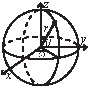
\includegraphics[width=25mm]{../vendor/kactl/content/math/sphericalCoordinates}
\end{center}
\[\begin{array}{cc}
x = r\sin\theta\cos\phi & r = \sqrt{x^2+y^2+z^2}\\
y = r\sin\theta\sin\phi & \theta = \textrm{acos}(z/\sqrt{x^2+y^2+z^2})\\
z = r\cos\theta & \phi = \textrm{atan2}(y,x)
\end{array}\]

\subsection{Derivatives/Integrals}
\begin{align*}
	\dfrac{d}{dx}\arcsin x = \dfrac{1}{\sqrt{1-x^2}} &&& \dfrac{d}{dx}\arccos x = -\dfrac{1}{\sqrt{1-x^2}} \\
	\dfrac{d}{dx}\tan x = 1+\tan^2 x &&& \dfrac{d}{dx}\arctan x = \dfrac{1}{1+x^2} \\
	\int\tan ax = -\dfrac{\ln|\cos ax|}{a} &&& \int x\sin ax = \dfrac{\sin ax-ax \cos ax}{a^2} \\
	\int e^{-x^2} = \frac{\sqrt \pi}{2} \text{erf}(x) &&& \int xe^{ax}dx = \frac{e^{ax}}{a^2}(ax-1)
\end{align*}

Integration by parts:
\[\int_a^bf(x)g(x)dx = [F(x)g(x)]_a^b-\int_a^bF(x)g'(x)dx\]

\subsection{Sums}
\[ c^a + c^{a+1} + \dots + c^{b} = \frac{c^{b+1} - c^a}{c-1}, c \neq 1 \]
\begin{align*}
	1 + 2 + 3 + \dots + n &= \frac{n(n+1)}{2} \\
	1^2 + 2^2 + 3^2 + \dots + n^2 &= \frac{n(2n+1)(n+1)}{6} \\
	1^3 + 2^3 + 3^3 + \dots + n^3 &= \frac{n^2(n+1)^2}{4} \\
	1^4 + 2^4 + 3^4 + \dots + n^4 &= \frac{n(n+1)(2n+1)(3n^2 + 3n - 1)}{30} \\
\end{align*}

\subsection{Series}
$$e^x = 1+x+\frac{x^2}{2!}+\frac{x^3}{3!}+\dots,\,(-\infty<x<\infty)$$
$$\ln(1+x) = x-\frac{x^2}{2}+\frac{x^3}{3}-\frac{x^4}{4}+\dots,\,(-1<x\leq1)$$
$$\sqrt{1+x} = 1+\frac{x}{2}-\frac{x^2}{8}+\frac{2x^3}{32}-\frac{5x^4}{128}+\dots,\,(-1\leq x\leq1)$$
$$\sin x = x-\frac{x^3}{3!}+\frac{x^5}{5!}-\frac{x^7}{7!}+\dots,\,(-\infty<x<\infty)$$
$$\cos x = 1-\frac{x^2}{2!}+\frac{x^4}{4!}-\frac{x^6}{6!}+\dots,\,(-\infty<x<\infty)$$

\subsection{Probability theory}
Let $X$ be a discrete random variable with probability $p_X(x)$ of assuming the value $x$. It will then have an expected value (mean) $\mu=\mathbb{E}(X)=\sum_xxp_X(x)$ and variance $\sigma^2=V(X)=\mathbb{E}(X^2)-(\mathbb{E}(X))^2=\sum_x(x-\mathbb{E}(X))^2p_X(x)$ where $\sigma$ is the standard deviation. If $X$ is instead continuous it will have a probability density function $f_X(x)$ and the sums above will instead be integrals with $p_X(x)$ replaced by $f_X(x)$.

Expectation is linear:
\[\mathbb{E}(aX+bY) = a\mathbb{E}(X)+b\mathbb{E}(Y)\]
For independent $X$ and $Y$, \[V(aX+bY) = a^2V(X)+b^2V(Y).\]

\subsubsection{Discrete distributions}

\paragraph{Binomial distribution}
The number of successes in $n$ independent yes/no experiments, each which yields success with probability $p$ is $\textrm{Bin}(n,p),\,n=1,2,\dots,\, 0\leq p\leq1$.
\[p(k)=\binom{n}{k}p^k(1-p)^{n-k}\]
\[\mu = np,\,\sigma^2=np(1-p)\]
$\textrm{Bin}(n,p)$ is approximately $\textrm{Po}(np)$ for small $p$.

\paragraph{First success distribution}
The number of trials needed to get the first success in independent yes/no experiments, each which yields success with probability $p$ is $\textrm{Fs}(p),\,0\leq p\leq1$.
\[p(k)=p(1-p)^{k-1},\,k=1,2,\dots\]
\[\mu = \frac1p,\,\sigma^2=\frac{1-p}{p^2}\]

\paragraph{Poisson distribution}
The number of events occurring in a fixed period of time $t$ if these events occur with a known average rate $\kappa$ and independently of the time since the last event is $\textrm{Po}(\lambda),\,\lambda=t\kappa$.
\[p(k)=e^{-\lambda}\frac{\lambda^k}{k!}, k=0,1,2,\dots\]
\[\mu=\lambda,\,\sigma^2=\lambda\]

\subsubsection{Continuous distributions}

\paragraph{Uniform distribution}
If the probability density function is constant between $a$ and $b$ and 0 elsewhere it is $\textrm{U}(a,b),\,a<b$.
\[f(x) = \left\{
\begin{array}{cl}
\frac{1}{b-a} & a<x<b\\
0 & \textrm{otherwise}
\end{array}\right.\]
\[\mu=\frac{a+b}{2},\,\sigma^2=\frac{(b-a)^2}{12}\]

\paragraph{Exponential distribution}
The time between events in a Poisson process is $\textrm{Exp}(\lambda),\,\lambda>0$.
\[f(x) = \left\{
\begin{array}{cl}
\lambda e^{-\lambda x} & x\geq0\\
0 & x<0
\end{array}\right.\]
\[\mu=\frac{1}{\lambda},\,\sigma^2=\frac{1}{\lambda^2}\]

\paragraph{Normal distribution}
Most real random values with mean $\mu$ and variance $\sigma^2$ are well described by $\mathcal{N}(\mu,\sigma^2),\,\sigma>0$.
\[ f(x) = \frac{1}{\sqrt{2\pi\sigma^2}}e^{-\frac{(x-\mu)^2}{2\sigma^2}} \]
If $X_1 \sim \mathcal{N}(\mu_1,\sigma_1^2)$ and $X_2 \sim \mathcal{N}(\mu_2,\sigma_2^2)$ are independent, then
\[ aX_1 + bX_2 + c \sim \mathcal{N}(a\mu_1+b\mu_2+c,a^2\sigma_1^2+b^2\sigma_2^2) \]

\subsection{Markov chains}
A \emph{Markov chain} is a discrete random process with the property that the next state depends only on the current state.
Let $X_1,X_2,\ldots$ be a sequence of random variables generated by the Markov process.
Then there is a transition matrix $\mathbf{P} = (p_{ij})$, with $p_{ij} = \Pr(X_n = i | X_{n-1} = j)$,
and $\mathbf{p}^{(n)} = \mathbf P^n \mathbf p^{(0)}$ is the probability distribution for $X_n$ (i.e., $p^{(n)}_i = \Pr(X_n = i)$),
where $\mathbf{p}^{(0)}$ is the initial distribution.

$\mathbf{\pi}$ is a stationary distribution if $\mathbf{\pi} = \mathbf{P \pi}$.
If the Markov chain is \emph{irreducible} (it is possible to get to any state from any state),
then $\pi_i = \frac{1}{\mathbb{E}(T_i)}$ where $\mathbb{E}(T_i)$  is the expected time between two visits in state $i$.
$\pi_j/\pi_i$ is the expected number of visits in state $j$ between two visits in state $i$.

For a connected, undirected and non-bipartite graph, where the transition probability is uniform among all neighbors, $\pi_i$ is proportional to node $i$'s degree.

A Markov chain is \emph{ergodic} if the asymptotic distribution is independent of the initial distribution.
A finite Markov chain is ergodic iff it is irreducible and \emph{aperiodic} (i.e., the gcd of cycle lengths is 1).
$\lim_{k\rightarrow\infty}\mathbf{P}^k = \mathbf{1}\pi$.

A Markov chain is an A-chain if the states can be partitioned into two sets $\mathbf{A}$ and $\mathbf{G}$, such that all states in $\mathbf{A}$ are absorbing ($p_{ii}=1$), and all states in $\mathbf{G}$ leads to an absorbing state in $\mathbf{A}$.
The probability for absorption in state $i\in\mathbf{A}$, when the initial state is $j$, is $a_{ij} = p_{ij}+\sum_{k\in\mathbf{G}} a_{ik}p_{kj}$.
The expected time until absorption, when the initial state is $i$, is $t_i = 1+\sum_{k\in\mathbf{G}}p_{ki}t_k$.
\Topic{Data structures \& collections}{data-structures}

\subsection{C++ containers: calls \& costs}
\ReferenceFact{Common calls} size(), empty(); begin()/end() delimit [first,last). Never dereference end(). front(), back(), top(), pop operations require nonempty containers. Most containers have clear(); stack, queue and priority\_queue do not.\par
\ReferenceFact{Costs} vector: index O(1), push\_back amortized O(1), middle insert/erase O(n). deque: index/end operations O(1), middle edits O(n). stack/queue: O(1) on default storage. Heap: top O(1), push/pop O(log n).\par
\ReferenceFact{Ordered vs hashed} set/map: lookup/insert/key erase O(log n); multiset allows duplicates; count/equal\_range also depend on matches. unordered\_set/map: expected O(1), worst O(n) per lookup/update; adversarial hashes can be slow. Use member lower\_bound on trees; std::lower\_bound can take O(n) iterator steps.\par
\ReferenceFact{Iterator lifetime} vector reallocation invalidates all iterators/references; erase invalidates at/after the position. Tree insert preserves iterators, erase invalidates only erased elements. Hash rehash invalidates iterators. Avoid modifying a container while range-iterating unless validity is guaranteed.\par
\Snippet{C++ container API}{C++}{Independent call examples; replace values/types as needed. bitset\textless{}N\textgreater{} uses a compile-time N; bitwise operations process machine words. C++17 membership: find(x) != end() or count(x).}
\lstinputlisting[language={C++}]{../topics/collections/cpp_containers.hpp}
\subsection{Arrays \& collections}
\TopicNote{Hash tables: expected O(1) lookup/insert/remove. Java hash iteration costs O(size+capacity). Python dict preserves insertion order; hash sets and Java HashMap have no guaranteed order. Array/list indexing is O(1); append is amortized O(1); middle insertion/removal and value search are O(n). Java generics use wrappers (Integer, not int).}
\Snippet{Arrays, matrix, sort and search}{Java}{Arrays are fixed-size and zero-initialized (objects: null). Arrays.sort also accepts String[]. binarySearch requires the same ordering used to sort; an absent key returns -(insertion point)-1. Iterate each row's length for ragged matrices.}
\lstinputlisting[language={Java}]{../topics/collections/ArraysReference.java}
\Snippet{Lists and primitive arrays}{Python}{list is dynamic; array('i') stores C signed integers and can also append/pop. rows and cols must be nonnegative. Use independent row lists: [[0]*cols]*rows aliases rows.}
\lstinputlisting[language={Python}]{../topics/collections/arrays.py}
\Snippet{ArrayList}{Java}{remove(int) removes by index; remove(Object) removes the first equal value. get/set/remove indices must exist; insertion allows index size().}
\lstinputlisting[language={Java}]{../topics/collections/Lists.java}
\Snippet{Hash set}{Python}{Elements must be hashable. remove raises KeyError if absent; discard does not. pop removes an arbitrary element and raises KeyError on an empty set.}
\lstinputlisting[language={Python}]{../topics/collections/sets.py}
\Snippet{HashSet}{Java}{add/remove return whether the set changed. Duplicate insertion is ignored. Custom keys need consistent equals and hashCode.}
\lstinputlisting[language={Java}]{../topics/collections/Sets.java}
\Snippet{Dictionary}{Python}{Keys must be hashable. d[key] raises KeyError if missing; get(key, fallback) is safe. Assignment and update overwrite existing values. Do not change dictionary size during iteration.}
\lstinputlisting[language={Python}]{../topics/collections/maps.py}
\Snippet{HashMap}{Java}{put/remove return the previous value, or null if absent. get can return null; unboxing null throws. containsValue is O(n). getOrDefault uses the fallback only for absent keys, not keys mapped to null.}
\lstinputlisting[language={Java}]{../topics/collections/Maps.java}
\Snippet{Queue, stack and deque}{Java}{FIFO: offer/poll; LIFO: push/pop. ArrayDeque rejects null. peek/poll return null on empty; pop/removeFirst/removeLast throw. End insertions/removals are amortized O(1).}
\lstinputlisting[language={Java}]{../topics/collections/Queues.java}


\KactlSnippet{OrderStatisticTree.h}{782797, 16 lines}
\defdescription{A set (not multiset!) with support for finding the n'th
element, and finding the index of an element.
To get a map, change \texttt{null\_type}.}
\deftime{\bigo{\log N}}
\begin{lstlisting}[language=C++]
#include <bits/extc++.h>
using namespace __gnu_pbds;

template<class T>
using Tree = tree<T, null_type, less<T>, rb_tree_tag,
    tree_order_statistics_node_update>;

void example() {
	Tree<int> t, t2; t.insert(8);
	auto it = t.insert(10).first;
	assert(it == t.lower_bound(9));
	assert(t.order_of_key(10) == 1);
	assert(t.order_of_key(11) == 2);
	assert(*t.find_by_order(0) == 8);
	t.join(t2); // assuming T < T2 or T > T2, merge t2 into t
}
\end{lstlisting}

\KactlSnippet{HashMap.h}{d77092, 7 lines}
\defdescription{Hash map with mostly the same API as unordered\_map, but \tilde
3x faster. Uses 1.5x memory.
Initial capacity must be a power of 2 (if provided).}
\begin{lstlisting}[language=C++]
#include <bits/extc++.h>
// To use most bits rather than just the lowest ones:
struct chash { // large odd number for C
	const uint64_t C = ll(4e18 * acos(0)) | 71;
	ll operator()(ll x) const { return __builtin_bswap64(x*C); }
};
__gnu_pbds::gp_hash_table<ll,int,chash> h({},{},{},{},{1<<16});
\end{lstlisting}

\KactlSnippet{SegmentTree.h}{0f4bdb, 19 lines}
\defdescription{Zero-indexed max-tree. Bounds are inclusive to the left and exclusive to the right.
Can be changed by modifying T, f and unit.}
\deftime{\bigo{\log N}}
\begin{lstlisting}[language=C++]
struct Tree {
	typedef int T;
	static constexpr T unit = INT_MIN;
	T f(T a, T b) { return max(a, b); } // (any associative fn)
	vector<T> s; int n;
	Tree(int n = 0, T def = unit) : s(2*n, def), n(n) {}
	void update(int pos, T val) {
		for (s[pos += n] = val; pos /= 2;)
			s[pos] = f(s[pos * 2], s[pos * 2 + 1]);
	}
	T query(int b, int e) { // query [b, e)
		T ra = unit, rb = unit;
		for (b += n, e += n; b < e; b /= 2, e /= 2) {
			if (b % 2) ra = f(ra, s[b++]);
			if (e % 2) rb = f(s[--e], rb);
		}
		return f(ra, rb);
	}
};
\end{lstlisting}

\KactlSnippet{LazySegmentTree.h}{34ecf5, 50 lines}
\defdescription{Segment tree with ability to add or set values of large intervals, and compute max of intervals.
Can be changed to other things.
Use with a bump allocator for better performance, and SmallPtr or implicit indices to save memory.}
\defusage{Node* tr = new Node(v, 0, sz(v));}
\deftime{\bigo{\log N}.}
\leftcaption{"../various/BumpAllocator.h"}
\begin{lstlisting}[language=C++]
const int inf = 1e9;
struct Node {
	Node *l = 0, *r = 0;
	int lo, hi, mset = inf, madd = 0, val = -inf;
	Node(int lo,int hi):lo(lo),hi(hi){} // Large interval of -inf
	Node(vi& v, int lo, int hi) : lo(lo), hi(hi) {
		if (lo + 1 < hi) {
			int mid = lo + (hi - lo)/2;
			l = new Node(v, lo, mid); r = new Node(v, mid, hi);
			val = max(l->val, r->val);
		}
		else val = v[lo];
	}
	int query(int L, int R) {
		if (R <= lo || hi <= L) return -inf;
		if (L <= lo && hi <= R) return val;
		push();
		return max(l->query(L, R), r->query(L, R));
	}
	void set(int L, int R, int x) {
		if (R <= lo || hi <= L) return;
		if (L <= lo && hi <= R) mset = val = x, madd = 0;
		else {
			push(), l->set(L, R, x), r->set(L, R, x);
			val = max(l->val, r->val);
		}
	}
	void add(int L, int R, int x) {
		if (R <= lo || hi <= L) return;
		if (L <= lo && hi <= R) {
			if (mset != inf) mset += x;
			else madd += x;
			val += x;
		}
		else {
			push(), l->add(L, R, x), r->add(L, R, x);
			val = max(l->val, r->val);
		}
	}
	void push() {
		if (!l) {
			int mid = lo + (hi - lo)/2;
			l = new Node(lo, mid); r = new Node(mid, hi);
		}
		if (mset != inf)
			l->set(lo,hi,mset), r->set(lo,hi,mset), mset = inf;
		else if (madd)
			l->add(lo,hi,madd), r->add(lo,hi,madd), madd = 0;
	}
};
\end{lstlisting}

\KactlSnippet{UnionFindRollback.h}{de4ad0, 21 lines}
\defdescription{Disjoint-set data structure with undo.
If undo is not needed, skip st, time() and rollback().}
\defusage{int t = uf.time(); ...; uf.rollback(t);}
\deftime{$\bigo{\log(N)}$}
\begin{lstlisting}[language=C++]
struct RollbackUF {
	vi e; vector<pii> st;
	RollbackUF(int n) : e(n, -1) {}
	int size(int x) { return -e[find(x)]; }
	int find(int x) { return e[x] < 0 ? x : find(e[x]); }
	int time() { return sz(st); }
	void rollback(int t) {
		for (int i = time(); i --> t;)
			e[st[i].first] = st[i].second;
		st.resize(t);
	}
	bool join(int a, int b) {
		a = find(a), b = find(b);
		if (a == b) return false;
		if (e[a] > e[b]) swap(a, b);
		st.push_back({a, e[a]});
		st.push_back({b, e[b]});
		e[a] += e[b]; e[b] = a;
		return true;
	}
};
\end{lstlisting}

\KactlSnippet{SubMatrix.h}{c59ada, 13 lines}
\defdescription{Calculate submatrix sums quickly, given upper-left and lower-right corners (half-open).}
\defusage{SubMatrix\ensuremath{<}int\ensuremath{>} m(matrix);\\
m.sum(0, 0, 2, 2); // top left 4 elements}
\deftime{\bigo{N^2 + Q}}
\begin{lstlisting}[language=C++]
template<class T>
struct SubMatrix {
	vector<vector<T>> p;
	SubMatrix(vector<vector<T>>& v) {
		int R = sz(v), C = sz(v[0]);
		p.assign(R+1, vector<T>(C+1));
		rep(r,0,R) rep(c,0,C)
			p[r+1][c+1] = v[r][c] + p[r][c+1] + p[r+1][c] - p[r][c];
	}
	T sum(int u, int l, int d, int r) {
		return p[d][r] - p[d][l] - p[u][r] + p[u][l];
	}
};
\end{lstlisting}

\KactlSnippet{Matrix.h}{4da5a2, 26 lines}
\defdescription{Basic operations on square matrices.}
\defusage{Matrix\ensuremath{<}int, 3\ensuremath{>} A;\\
A.d = \{\{\{\{1,2,3\}\}, \{\{4,5,6\}\}, \{\{7,8,9\}\}\}\};\\
array\ensuremath{<}int, 3\ensuremath{>} vec = \{1,2,3\};\\
vec = (A\ensuremath{\hat{\;}}N) * vec;}
\begin{lstlisting}[language=C++]
template<class T, int N> struct Matrix {
	typedef Matrix M;
	array<array<T, N>, N> d{};
	M operator*(const M& m) const {
		M a;
		rep(i,0,N) rep(j,0,N)
			rep(k,0,N) a.d[i][k] += d[i][j] * m.d[j][k];
		return a;
	}
	array<T, N> operator*(const array<T, N>& vec) const {
		array<T, N> ret{};
		rep(i,0,N) rep(j,0,N) ret[i] += d[i][j] * vec[j];
		return ret;
	}
	M operator^(ll p) const {
		assert(p >= 0);
		M a, b(*this);
		rep(i,0,N) a.d[i][i] = 1;
		while (p) {
			if (p&1) a = a*b;
			b = b*b;
			p >>= 1;
		}
		return a;
	}
};
\end{lstlisting}

\KactlSnippet{LineContainer.h}{8ec1c7, 30 lines}
\defdescription{Container where you can add lines of the form kx+m, and query maximum values at points x.
Useful for dynamic programming (``convex hull trick'').}
\deftime{\bigo{\log N}}
\begin{lstlisting}[language=C++]
struct Line {
	mutable ll k, m, p;
	bool operator<(const Line& o) const { return k < o.k; }
	bool operator<(ll x) const { return p < x; }
};

struct LineContainer : multiset<Line, less<>> {
	// (for doubles, use inf = 1/.0, div(a,b) = a/b)
	static const ll inf = LLONG_MAX;
	ll div(ll a, ll b) { // floored division
		return a / b - ((a ^ b) < 0 && a % b); }
	bool isect(iterator x, iterator y) {
		if (y == end()) return x->p = inf, 0;
		if (x->k == y->k) x->p = x->m > y->m ? inf : -inf;
		else x->p = div(y->m - x->m, x->k - y->k);
		return x->p >= y->p;
	}
	void add(ll k, ll m) {
		auto z = insert({k, m, 0}), y = z++, x = y;
		while (isect(y, z)) z = erase(z);
		if (x != begin() && isect(--x, y)) isect(x, y = erase(y));
		while ((y = x) != begin() && (--x)->p >= y->p)
			isect(x, erase(y));
	}
	ll query(ll x) {
		assert(!empty());
		auto l = *lower_bound(x);
		return l.k * x + l.m;
	}
};
\end{lstlisting}

\KactlSnippet{Treap.h}{1754b4, 53 lines}
\defdescription{A short self-balancing tree. It acts as a
sequential container with log-time splits/joins, and
is easy to augment with additional data.}
\deftime{$\bigo{\log N}$}
\begin{lstlisting}[language=C++]
struct Node {
	Node *l = 0, *r = 0;
	int val, y, c = 1;
	Node(int val) : val(val), y(rand()) {}
	void recalc();
};

int cnt(Node* n) { return n ? n->c : 0; }
void Node::recalc() { c = cnt(l) + cnt(r) + 1; }

template<class F> void each(Node* n, F f) {
	if (n) { each(n->l, f); f(n->val); each(n->r, f); }
}

pair<Node*, Node*> split(Node* n, int k) {
	if (!n) return {};
	if (cnt(n->l) >= k) { // "n->val >= k" for lower_bound(k)
		auto [L,R] = split(n->l, k);
		n->l = R;
		n->recalc();
		return {L, n};
	} else {
		auto [L,R] = split(n->r,k - cnt(n->l) - 1); // and just "k"
		n->r = L;
		n->recalc();
		return {n, R};
	}
}

Node* merge(Node* l, Node* r) {
	if (!l) return r;
	if (!r) return l;
	if (l->y > r->y) {
		l->r = merge(l->r, r);
		return l->recalc(), l;
	} else {
		r->l = merge(l, r->l);
		return r->recalc(), r;
	}
}

Node* ins(Node* t, Node* n, int pos) {
	auto [l,r] = split(t, pos);
	return merge(merge(l, n), r);
}

// Example application: move the range [l, r) to index k
void move(Node*& t, int l, int r, int k) {
	Node *a, *b, *c;
	tie(a,b) = split(t, l); tie(b,c) = split(b, r - l);
	if (k <= l) t = merge(ins(a, b, k), c);
	else t = merge(a, ins(c, b, k - r));
}
\end{lstlisting}

\KactlSnippet{FenwickTree.h}{e62fac, 22 lines}
\defdescription{Computes partial sums a[0] + a[1] + ... + a[pos - 1], and updates single elements a[i],
taking the difference between the old and new value.}
\deftime{Both operations are $\bigo{\log N}$.}
\begin{lstlisting}[language=C++]
struct FT {
	vector<ll> s;
	FT(int n) : s(n) {}
	void update(int pos, ll dif) { // a[pos] += dif
		for (; pos < sz(s); pos |= pos + 1) s[pos] += dif;
	}
	ll query(int pos) { // sum of values in [0, pos)
		ll res = 0;
		for (; pos > 0; pos &= pos - 1) res += s[pos-1];
		return res;
	}
	int lower_bound(ll sum) {// min pos st sum of [0, pos] >= sum
		// Returns n if no sum is >= sum, or -1 if empty sum is.
		if (sum <= 0) return -1;
		int pos = 0;
		for (int pw = 1 << 25; pw; pw >>= 1) {
			if (pos + pw <= sz(s) && s[pos + pw-1] < sum)
				pos += pw, sum -= s[pos-1];
		}
		return pos;
	}
};
\end{lstlisting}

\KactlSnippet{FenwickTree2d.h}{157f07, 22 lines}
\defdescription{Computes sums a[i,j] for all i\ensuremath{<}I, j\ensuremath{<}J, and increases single elements a[i,j].
Requires that the elements to be updated are known in advance (call fakeUpdate() before init()).}
\deftime{$\bigo{\log^2 N}$. (Use persistent segment trees for $\bigo{\log N}$.)}
\leftcaption{"FenwickTree.h"}
\begin{lstlisting}[language=C++]
struct FT2 {
	vector<vi> ys; vector<FT> ft;
	FT2(int limx) : ys(limx) {}
	void fakeUpdate(int x, int y) {
		for (; x < sz(ys); x |= x + 1) ys[x].push_back(y);
	}
	void init() {
		for (vi& v : ys) sort(all(v)), ft.emplace_back(sz(v));
	}
	int ind(int x, int y) {
		return (int)(lower_bound(all(ys[x]), y) - ys[x].begin()); }
	void update(int x, int y, ll dif) {
		for (; x < sz(ys); x |= x + 1)
			ft[x].update(ind(x, y), dif);
	}
	ll query(int x, int y) {
		ll sum = 0;
		for (; x; x &= x - 1)
			sum += ft[x-1].query(ind(x-1, y));
		return sum;
	}
};
\end{lstlisting}

\KactlSnippet{RMQ.h}{510c32, 16 lines}
\defdescription{Range Minimum Queries on an array. Returns
min(V[a], V[a + 1], ... V[b - 1]) in constant time.}
\defusage{RMQ rmq(values);\\
rmq.query(inclusive, exclusive);}
\deftime{$\bigo{|V| \log |V| + Q}$}
\begin{lstlisting}[language=C++]
template<class T>
struct RMQ {
	vector<vector<T>> jmp;
	RMQ(const vector<T>& V) : jmp(1, V) {
		for (int pw = 1, k = 1; pw * 2 <= sz(V); pw *= 2, ++k) {
			jmp.emplace_back(sz(V) - pw * 2 + 1);
			rep(j,0,sz(jmp[k]))
				jmp[k][j] = min(jmp[k - 1][j], jmp[k - 1][j + pw]);
		}
	}
	T query(int a, int b) {
		assert(a < b); // or return inf if a == b
		int dep = 31 - __builtin_clz(b - a);
		return min(jmp[dep][a], jmp[dep][b - (1 << dep)]);
	}
};
\end{lstlisting}

\KactlSnippet{MoQueries.h}{a12ef4, 49 lines}
\defdescription{Answer interval or tree path queries by finding an approximate TSP through the queries,
and moving from one query to the next by adding/removing points at the ends.
If values are on tree edges, change \texttt{step} to add/remove the edge $(a, c)$ and remove the initial \texttt{add} call (but keep \texttt{in}).}
\deftime{\bigo{N \sqrt Q}}
\begin{lstlisting}[language=C++]
void add(int ind, int end) { ... } // add a[ind] (end = 0 or 1)
void del(int ind, int end) { ... } // remove a[ind]
int calc() { ... } // compute current answer

vi mo(vector<pii> Q) {
	int L = 0, R = 0, blk = 350; // ~N/sqrt(Q)
	vi s(sz(Q)), res = s;
#define K(x) pii(x.first/blk, x.second ^ -(x.first/blk & 1))
	iota(all(s), 0);
	sort(all(s), [&](int s, int t){ return K(Q[s]) < K(Q[t]); });
	for (int qi : s) {
		pii q = Q[qi];
		while (L > q.first) add(--L, 0);
		while (R < q.second) add(R++, 1);
		while (L < q.first) del(L++, 0);
		while (R > q.second) del(--R, 1);
		res[qi] = calc();
	}
	return res;
}

vi moTree(vector<array<int, 2>> Q, vector<vi>& ed, int root=0){
	int N = sz(ed), pos[2] = {}, blk = 350; // ~N/sqrt(Q)
	vi s(sz(Q)), res = s, I(N), L(N), R(N), in(N), par(N);
	add(0, 0), in[0] = 1;
	auto dfs = [&](int x, int p, int dep, auto& f) -> void {
		par[x] = p;
		L[x] = N;
		if (dep) I[x] = N++;
		for (int y : ed[x]) if (y != p) f(y, x, !dep, f);
		if (!dep) I[x] = N++;
		R[x] = N;
	};
	dfs(root, -1, 0, dfs);
#define K(x) pii(I[x[0]] / blk, I[x[1]] ^ -(I[x[0]] / blk & 1))
	iota(all(s), 0);
	sort(all(s), [&](int s, int t){ return K(Q[s]) < K(Q[t]); });
	for (int qi : s) rep(end,0,2) {
		int &a = pos[end], b = Q[qi][end], i = 0;
#define step(c) { if (in[c]) { del(a, end); in[a] = 0; } \
                  else { add(c, end); in[c] = 1; } a = c; }
		while (!(L[b] <= L[a] && R[a] <= R[b]))
			I[i++] = b, b = par[b];
		while (a != b) step(par[a]);
		while (i--) step(I[i]);
		if (end) res[qi] = calc();
	}
	return res;
}
\end{lstlisting}

\Topic{Numerical algorithms}{numerical}



\subsection{Polynomials and recurrences}
  \KactlSnippet{Polynomial.h}{c9b7b0, 17 lines}
\begin{lstlisting}[language=C++]
struct Poly {
	vector<double> a;
	double operator()(double x) const {
		double val = 0;
		for (int i = sz(a); i--;) (val *= x) += a[i];
		return val;
	}
	void diff() {
		rep(i,1,sz(a)) a[i-1] = i*a[i];
		a.pop_back();
	}
	void divroot(double x0) {
		double b = a.back(), c; a.back() = 0;
		for(int i=sz(a)-1; i--;) c = a[i], a[i] = a[i+1]*x0+b, b=c;
		a.pop_back();
	}
};
\end{lstlisting}

  \KactlSnippet{PolyRoots.h}{b00bfe, 23 lines}
\defdescription{Finds the real roots to a polynomial.}
\defusage{polyRoots(\{\{2,-3,1\}\},-1e9,1e9) // solve x\ensuremath{\hat{\;}}2-3x+2 = 0}
\deftime{\bigo{n^2 \log(1/\epsilon)}}
\leftcaption{"Polynomial.h"}
\begin{lstlisting}[language=C++]
vector<double> polyRoots(Poly p, double xmin, double xmax) {
	if (sz(p.a) == 2) { return {-p.a[0]/p.a[1]}; }
	vector<double> ret;
	Poly der = p;
	der.diff();
	auto dr = polyRoots(der, xmin, xmax);
	dr.push_back(xmin-1);
	dr.push_back(xmax+1);
	sort(all(dr));
	rep(i,0,sz(dr)-1) {
		double l = dr[i], h = dr[i+1];
		bool sign = p(l) > 0;
		if (sign ^ (p(h) > 0)) {
			rep(it,0,60) { // while (h - l > 1e-8)
				double m = (l + h) / 2, f = p(m);
				if ((f <= 0) ^ sign) l = m;
				else h = m;
			}
			ret.push_back((l + h) / 2);
		}
	}
	return ret;
}
\end{lstlisting}

  \KactlSnippet{PolyInterpolate.h}{08bf48, 13 lines}
\defdescription{Given $n$ points (x[i], y[i]), computes an n-1-degree polynomial $p$ that
passes through them: $p(x) = a[0]*x^0 + ... + a[n-1]*x^{n-1}$.
For numerical precision, pick $x[k] = c*\cos(k/(n-1)*\pi), k=0 \dots n-1$.}
\deftime{\bigo{n^2}}
\begin{lstlisting}[language=C++]
typedef vector<double> vd;
vd interpolate(vd x, vd y, int n) {
	vd res(n), temp(n);
	rep(k,0,n-1) rep(i,k+1,n)
		y[i] = (y[i] - y[k]) / (x[i] - x[k]);
	double last = 0; temp[0] = 1;
	rep(k,0,n) rep(i,0,n) {
		res[i] += y[k] * temp[i];
		swap(last, temp[i]);
		temp[i] -= last * x[k];
	}
	return res;
}
\end{lstlisting}

  \KactlSnippet{BerlekampMassey.h}{96548b, 20 lines}
\defdescription{Recovers any $n$-order linear recurrence relation from the first
$2n$ terms of the recurrence.
Useful for guessing linear recurrences after brute-forcing the first terms.
Should work on any field, but numerical stability for floats is not guaranteed.
Output will have size $\le n$.}
\defusage{berlekampMassey(\{0, 1, 1, 3, 5, 11\}) // \{1, 2\}}
\deftime{\bigo{N^2}}
\leftcaption{"../number-theory/ModPow.h"}
\begin{lstlisting}[language=C++]
vector<ll> berlekampMassey(vector<ll> s) {
	int n = sz(s), L = 0, m = 0;
	vector<ll> C(n), B(n), T;
	C[0] = B[0] = 1;

	ll b = 1;
	rep(i,0,n) { ++m;
		ll d = s[i] % mod;
		rep(j,1,L+1) d = (d + C[j] * s[i - j]) % mod;
		if (!d) continue;
		T = C; ll coef = d * modpow(b, mod-2) % mod;
		rep(j,m,n) C[j] = (C[j] - coef * B[j - m]) % mod;
		if (2 * L > i) continue;
		L = i + 1 - L; B = T; b = d; m = 0;
	}

	C.resize(L + 1); C.erase(C.begin());
	for (ll& x : C) x = (mod - x) % mod;
	return C;
}
\end{lstlisting}

  \KactlSnippet{LinearRecurrence.h}{f4e444, 26 lines}
\defdescription{Generates the $k$'th term of an $n$-order
linear recurrence $S[i] = \sum_j S[i-j-1]tr[j]$,
given $S[0 \ldots \ge n-1]$ and $tr[0 \ldots n-1]$.
Faster than matrix multiplication.
Useful together with Berlekamp--Massey.}
\defusage{linearRec(\{0, 1\}, \{1, 1\}, k) // k'th Fibonacci number}
\deftime{\bigo{n^2 \log k}}
\begin{lstlisting}[language=C++]
typedef vector<ll> Poly;
ll linearRec(Poly S, Poly tr, ll k) {
	int n = sz(tr);

	auto combine = [&](Poly a, Poly b) {
		Poly res(n * 2 + 1);
		rep(i,0,n+1) rep(j,0,n+1)
			res[i + j] = (res[i + j] + a[i] * b[j]) % mod;
		for (int i = 2 * n; i > n; --i) rep(j,0,n)
			res[i - 1 - j] = (res[i - 1 - j] + res[i] * tr[j]) % mod;
		res.resize(n + 1);
		return res;
	};

	Poly pol(n + 1), e(pol);
	pol[0] = e[1] = 1;

	for (++k; k; k /= 2) {
		if (k % 2) pol = combine(pol, e);
		e = combine(e, e);
	}

	ll res = 0;
	rep(i,0,n) res = (res + pol[i + 1] * S[i]) % mod;
	return res;
}
\end{lstlisting}


\subsection{Optimization}
  \KactlSnippet{GoldenSectionSearch.h}{31d45b, 14 lines}
\defdescription{Finds the argument minimizing the function $f$ in the interval $[a,b]$
assuming $f$ is unimodal on the interval, i.e. has only one local minimum and no local
maximum. The maximum error in the result is $eps$. Works equally well for maximization
with a small change in the code. See TernarySearch.h in the Various chapter for a
discrete version.}
\defusage{double func(double x) \{ return 4+x+.3*x*x; \}\\
double xmin = gss(-1000,1000,func);}
\deftime{\bigo{\log((b-a) / \epsilon)}}
\begin{lstlisting}[language=C++]
double gss(double a, double b, double (*f)(double)) {
	double r = (sqrt(5)-1)/2, eps = 1e-7;
	double x1 = b - r*(b-a), x2 = a + r*(b-a);
	double f1 = f(x1), f2 = f(x2);
	while (b-a > eps)
		if (f1 < f2) { //change to > to find maximum
			b = x2; x2 = x1; f2 = f1;
			x1 = b - r*(b-a); f1 = f(x1);
		} else {
			a = x1; x1 = x2; f1 = f2;
			x2 = a + r*(b-a); f2 = f(x2);
		}
	return a;
}
\end{lstlisting}

  \KactlSnippet{HillClimbing.h}{8eeeaf, 14 lines}
\defdescription{Poor man's optimization for unimodal functions.}
\begin{lstlisting}[language=C++]
typedef array<double, 2> P;

template<class F> pair<double, P> hillClimb(P start, F f) {
	pair<double, P> cur(f(start), start);
	for (double jmp = 1e9; jmp > 1e-20; jmp /= 2) {
		rep(j,0,100) rep(dx,-1,2) rep(dy,-1,2) {
			P p = cur.second;
			p[0] += dx*jmp;
			p[1] += dy*jmp;
			cur = min(cur, make_pair(f(p), p));
		}
	}
	return cur;
}
\end{lstlisting}

  \KactlSnippet{Integrate.h}{4756fc, 7 lines}
\defdescription{Simple integration of a function over an interval using
Simpson's rule. The error should be proportional to $h^4$, although in
practice you will want to verify that the result is stable to desired
precision when epsilon changes.}
\begin{lstlisting}[language=C++]
template<class F>
double quad(double a, double b, F f, const int n = 1000) {
	double h = (b - a) / 2 / n, v = f(a) + f(b);
	rep(i,1,n*2)
		v += f(a + i*h) * (i&1 ? 4 : 2);
	return v * h / 3;
}
\end{lstlisting}

  \KactlSnippet{IntegrateAdaptive.h}{92dd79, 15 lines}
\defdescription{Fast integration using an adaptive Simpson's rule.}
\defusage{double sphereVolume = quad(-1, 1, [](double x) \{\\
return quad(-1, 1, [\&](double y) \{\\
return quad(-1, 1, [\&](double z) \{\\
return x*x + y*y + z*z \ensuremath{<} 1; \});\});\});}
\begin{lstlisting}[language=C++]
typedef double d;
#define S(a,b) (f(a) + 4*f((a+b) / 2) + f(b)) * (b-a) / 6

template <class F>
d rec(F& f, d a, d b, d eps, d S) {
	d c = (a + b) / 2;
	d S1 = S(a, c), S2 = S(c, b), T = S1 + S2;
	if (abs(T - S) <= 15 * eps || b - a < 1e-10)
		return T + (T - S) / 15;
	return rec(f, a, c, eps / 2, S1) + rec(f, c, b, eps / 2, S2);
}
template<class F>
d quad(d a, d b, F f, d eps = 1e-8) {
	return rec(f, a, b, eps, S(a, b));
}
\end{lstlisting}

  \KactlSnippet{Simplex.h}{aa8530, 68 lines}
\defdescription{Solves a general linear maximization problem: maximize $c^T x$ subject to $Ax \le b$, $x \ge 0$.
Returns -inf if there is no solution, inf if there are arbitrarily good solutions, or the maximum value of $c^T x$ otherwise.
The input vector is set to an optimal $x$ (or in the unbounded case, an arbitrary solution fulfilling the constraints).
Numerical stability is not guaranteed. For better performance, define variables such that $x = 0$ is viable.}
\defusage{vvd A = \{\{1,-1\}, \{-1,1\}, \{-1,-2\}\};\\
vd b = \{1,1,-4\}, c = \{-1,-1\}, x;\\
T val = LPSolver(A, b, c).solve(x);}
\deftime{\bigo{NM * \#pivots}, where a pivot may be e.g. an edge relaxation. \bigo{2^n} in the general case.}
\begin{lstlisting}[language=C++]
typedef double T; // long double, Rational, double + mod<P>...
typedef vector<T> vd;
typedef vector<vd> vvd;

const T eps = 1e-8, inf = 1/.0;
#define MP make_pair
#define ltj(X) if(s == -1 || MP(X[j],N[j]) < MP(X[s],N[s])) s=j

struct LPSolver {
	int m, n;
	vi N, B;
	vvd D;

	LPSolver(const vvd& A, const vd& b, const vd& c) :
		m(sz(b)), n(sz(c)), N(n+1), B(m), D(m+2, vd(n+2)) {
			rep(i,0,m) rep(j,0,n) D[i][j] = A[i][j];
			rep(i,0,m) { B[i] = n+i; D[i][n] = -1; D[i][n+1] = b[i];}
			rep(j,0,n) { N[j] = j; D[m][j] = -c[j]; }
			N[n] = -1; D[m+1][n] = 1;
		}

	void pivot(int r, int s) {
		T *a = D[r].data(), inv = 1 / a[s];
		rep(i,0,m+2) if (i != r && abs(D[i][s]) > eps) {
			T *b = D[i].data(), inv2 = b[s] * inv;
			rep(j,0,n+2) b[j] -= a[j] * inv2;
			b[s] = a[s] * inv2;
		}
		rep(j,0,n+2) if (j != s) D[r][j] *= inv;
		rep(i,0,m+2) if (i != r) D[i][s] *= -inv;
		D[r][s] = inv;
		swap(B[r], N[s]);
	}

	bool simplex(int phase) {
		int x = m + phase - 1;
		for (;;) {
			int s = -1;
			rep(j,0,n+1) if (N[j] != -phase) ltj(D[x]);
			if (D[x][s] >= -eps) return true;
			int r = -1;
			rep(i,0,m) {
				if (D[i][s] <= eps) continue;
				if (r == -1 || MP(D[i][n+1] / D[i][s], B[i])
				             < MP(D[r][n+1] / D[r][s], B[r])) r = i;
			}
			if (r == -1) return false;
			pivot(r, s);
		}
	}

	T solve(vd &x) {
		int r = 0;
		rep(i,1,m) if (D[i][n+1] < D[r][n+1]) r = i;
		if (D[r][n+1] < -eps) {
			pivot(r, n);
			if (!simplex(2) || D[m+1][n+1] < -eps) return -inf;
			rep(i,0,m) if (B[i] == -1) {
				int s = 0;
				rep(j,1,n+1) ltj(D[i]);
				pivot(i, s);
			}
		}
		bool ok = simplex(1); x = vd(n);
		rep(i,0,m) if (B[i] < n) x[B[i]] = D[i][n+1];
		return ok ? D[m][n+1] : inf;
	}
};
\end{lstlisting}


\subsection{Matrices}
  \KactlSnippet{Determinant.h}{bd5cec, 15 lines}
\defdescription{Calculates determinant of a matrix. Destroys the matrix.}
\deftime{$\bigo{N^3}$}
\begin{lstlisting}[language=C++]
double det(vector<vector<double>>& a) {
	int n = sz(a); double res = 1;
	rep(i,0,n) {
		int b = i;
		rep(j,i+1,n) if (fabs(a[j][i]) > fabs(a[b][i])) b = j;
		if (i != b) swap(a[i], a[b]), res *= -1;
		res *= a[i][i];
		if (res == 0) return 0;
		rep(j,i+1,n) {
			double v = a[j][i] / a[i][i];
			if (v != 0) rep(k,i+1,n) a[j][k] -= v * a[i][k];
		}
	}
	return res;
}
\end{lstlisting}

  \KactlSnippet{IntDeterminant.h}{3313dc, 18 lines}
\defdescription{Calculates determinant using modular arithmetics.
Modulos can also be removed to get a pure-integer version.}
\deftime{$\bigo{N^3}$}
\begin{lstlisting}[language=C++]
const ll mod = 12345;
ll det(vector<vector<ll>>& a) {
	int n = sz(a); ll ans = 1;
	rep(i,0,n) {
		rep(j,i+1,n) {
			while (a[j][i] != 0) { // gcd step
				ll t = a[i][i] / a[j][i];
				if (t) rep(k,i,n)
					a[i][k] = (a[i][k] - a[j][k] * t) % mod;
				swap(a[i], a[j]);
				ans *= -1;
			}
		}
		ans = ans * a[i][i] % mod;
		if (!ans) return 0;
	}
	return (ans + mod) % mod;
}
\end{lstlisting}

  \KactlSnippet{SolveLinear.h}{44c9ab, 38 lines}
\defdescription{Solves $A * x = b$. If there are multiple solutions, an arbitrary one is returned.
Returns rank, or -1 if no solutions. Data in $A$ and $b$ is lost.}
\deftime{\bigo{n^2 m}}
\begin{lstlisting}[language=C++]
typedef vector<double> vd;
const double eps = 1e-12;

int solveLinear(vector<vd>& A, vd& b, vd& x) {
	int n = sz(A), m = sz(x), rank = 0, br, bc;
	if (n) assert(sz(A[0]) == m);
	vi col(m); iota(all(col), 0);

	rep(i,0,n) {
		double v, bv = 0;
		rep(r,i,n) rep(c,i,m)
			if ((v = fabs(A[r][c])) > bv)
				br = r, bc = c, bv = v;
		if (bv <= eps) {
			rep(j,i,n) if (fabs(b[j]) > eps) return -1;
			break;
		}
		swap(A[i], A[br]);
		swap(b[i], b[br]);
		swap(col[i], col[bc]);
		rep(j,0,n) swap(A[j][i], A[j][bc]);
		bv = 1/A[i][i];
		rep(j,i+1,n) {
			double fac = A[j][i] * bv;
			b[j] -= fac * b[i];
			rep(k,i+1,m) A[j][k] -= fac*A[i][k];
		}
		rank++;
	}

	x.assign(m, 0);
	for (int i = rank; i--;) {
		b[i] /= A[i][i];
		x[col[i]] = b[i];
		rep(j,0,i) b[j] -= A[j][i] * b[i];
	}
	return rank; // (multiple solutions if rank < m)
}
\end{lstlisting}

  \KactlSnippet{SolveLinear2.h}{08e495, 7 lines}
\defdescription{To get all uniquely determined values of $x$ back from SolveLinear, make the following changes:}
\leftcaption{"SolveLinear.h"}
\begin{lstlisting}[language=C++]
rep(j,0,n) if (j != i) // instead of rep(j,i+1,n)
// ... then at the end:
x.assign(m, undefined);
rep(i,0,rank) {
	rep(j,rank,m) if (fabs(A[i][j]) > eps) goto fail;
	x[col[i]] = b[i] / A[i][i];
fail:; }
\end{lstlisting}

  \KactlSnippet{SolveLinearBinary.h}{fa2d7a, 34 lines}
\defdescription{Solves $Ax = b$ over $\mathbb F_2$. If there are multiple solutions, one is returned arbitrarily.
Returns rank, or -1 if no solutions. Destroys $A$ and $b$.}
\deftime{\bigo{n^2 m}}
\begin{lstlisting}[language=C++]
typedef bitset<1000> bs;

int solveLinear(vector<bs>& A, vi& b, bs& x, int m) {
	int n = sz(A), rank = 0, br;
	assert(m <= sz(x));
	vi col(m); iota(all(col), 0);
	rep(i,0,n) {
		for (br=i; br<n; ++br) if (A[br].any()) break;
		if (br == n) {
			rep(j,i,n) if(b[j]) return -1;
			break;
		}
		int bc = (int)A[br]._Find_next(i-1);
		swap(A[i], A[br]);
		swap(b[i], b[br]);
		swap(col[i], col[bc]);
		rep(j,0,n) if (A[j][i] != A[j][bc]) {
			A[j].flip(i); A[j].flip(bc);
		}
		rep(j,i+1,n) if (A[j][i]) {
			b[j] ^= b[i];
			A[j] ^= A[i];
		}
		rank++;
	}

	x = bs();
	for (int i = rank; i--;) {
		if (!b[i]) continue;
		x[col[i]] = 1;
		rep(j,0,i) b[j] ^= A[j][i];
	}
	return rank; // (multiple solutions if rank < m)
}
\end{lstlisting}

  \KactlSnippet{MatrixInverse.h}{ebfff6, 35 lines}
\defdescription{Invert matrix $A$. Returns rank; result is stored in $A$ unless singular (rank \ensuremath{<} n).
Can easily be extended to prime moduli; for prime powers, repeatedly
set $A^{-1} = A^{-1} (2I - AA^{-1})\  (\text{mod }p^k)$ where $A^{-1}$ starts as
the inverse of A mod p, and k is doubled in each step.}
\deftime{\bigo{n^3}}
\begin{lstlisting}[language=C++]
int matInv(vector<vector<double>>& A) {
	int n = sz(A); vi col(n);
	vector<vector<double>> tmp(n, vector<double>(n));
	rep(i,0,n) tmp[i][i] = 1, col[i] = i;

	rep(i,0,n) {
		int r = i, c = i;
		rep(j,i,n) rep(k,i,n)
			if (fabs(A[j][k]) > fabs(A[r][c]))
				r = j, c = k;
		if (fabs(A[r][c]) < 1e-12) return i;
		A[i].swap(A[r]); tmp[i].swap(tmp[r]);
		rep(j,0,n)
			swap(A[j][i], A[j][c]), swap(tmp[j][i], tmp[j][c]);
		swap(col[i], col[c]);
		double v = A[i][i];
		rep(j,i+1,n) {
			double f = A[j][i] / v;
			A[j][i] = 0;
			rep(k,i+1,n) A[j][k] -= f*A[i][k];
			rep(k,0,n) tmp[j][k] -= f*tmp[i][k];
		}
		rep(j,i+1,n) A[i][j] /= v;
		rep(j,0,n) tmp[i][j] /= v;
		A[i][i] = 1;
	}

	for (int i = n-1; i > 0; --i) rep(j,0,i) {
		double v = A[j][i];
		rep(k,0,n) tmp[j][k] -= v*tmp[i][k];
	}

	rep(i,0,n) rep(j,0,n) A[col[i]][col[j]] = tmp[i][j];
	return n;
}
\end{lstlisting}

  \KactlSnippet{Tridiagonal.h}{8f9fa8, 26 lines}
\defdescription{$x=\textrm{tridiagonal}(d,p,q,b)$ solves the equation system
\FitDisplay{
\left(\begin{array}{c}b_0\\b_1\\b_2\\b_3\\\vdots\\b_{n-1}\end{array}\right) =
\left(\begin{array}{cccccc}
d_0 & p_0 & 0 & 0 & \cdots & 0\\
q_0 & d_1 & p_1 & 0 & \cdots & 0\\
0 & q_1 & d_2 & p_2 & \cdots & 0\\
\vdots & \vdots & \ddots & \ddots & \ddots & \vdots\\
0 & 0 & \cdots & q_{n-3} & d_{n-2} & p_{n-2}\\
0 & 0 & \cdots & 0 & q_{n-2} & d_{n-1}\\
\end{array}\right)
\left(\begin{array}{c}x_0\\x_1\\x_2\\x_3\\\vdots\\x_{n-1}\end{array}\right).
}

This is useful for solving problems on the type
\FitDisplay{ a_i=b_ia_{i-1}+c_ia_{i+1}+d_i,\,1\leq i\leq n, }
where $a_0$, $a_{n+1}$, $b_i$, $c_i$ and $d_i$ are known. $a$ can then be obtained from
\FitDisplay{\begin{aligned}
\{a_i\}=\textrm{tridiagonal}(&\{1,-1,-1,...,-1,1\}, \{0,c_1,c_2,\dots,c_n\},\\
&\{b_1,b_2,\dots,b_n,0\}, \{a_0,d_1,d_2,\dots,d_n,a_{n+1}\}).
\end{aligned}}
Fails if the solution is not unique.

If $|d_i| \ensuremath{>} |p_i| + |q_{i-1}|$ for all $i$, or $|d_i| \ensuremath{>} |p_{i-1}| + |q_i|$, or the matrix is positive definite,
the algorithm is numerically stable and neither \texttt{tr} nor the check for \texttt{diag[i] == 0} is needed.}
\deftime{\bigo{N}}
\begin{lstlisting}[language=C++]
typedef double T;
vector<T> tridiagonal(vector<T> diag, const vector<T>& super,
		const vector<T>& sub, vector<T> b) {
	int n = sz(b); vi tr(n);
	rep(i,0,n-1) {
		if (abs(diag[i]) < 1e-9 * abs(super[i])) { // diag[i] == 0
			b[i+1] -= b[i] * diag[i+1] / super[i];
			if (i+2 < n) b[i+2] -= b[i] * sub[i+1] / super[i];
			diag[i+1] = sub[i]; tr[++i] = 1;
		} else {
			diag[i+1] -= super[i]*sub[i]/diag[i];
			b[i+1] -= b[i]*sub[i]/diag[i];
		}
	}
	for (int i = n; i--;) {
		if (tr[i]) {
			swap(b[i], b[i-1]);
			diag[i-1] = diag[i];
			b[i] /= super[i-1];
		} else {
			b[i] /= diag[i];
			if (i) b[i-1] -= b[i]*super[i-1];
		}
	}
	return b;
}
\end{lstlisting}


\subsection{Fourier transforms}
	\KactlSnippet{FastFourierTransform.h}{00ced6, 35 lines}
\defdescription{fft(a) computes $\hat f(k) = \sum_x a[x] \exp(2\pi i \cdot k x / N)$ for all $k$. N must be a power of 2.
Useful for convolution:
\texttt{conv(a, b) = c}, where $c[x] = \sum a[i]b[x-i]$.
For convolution of complex numbers or more than two vectors: FFT, multiply
pointwise, divide by n, reverse(start+1, end), FFT back.
Rounding is safe if $(\sum a_i^2 + \sum b_i^2)\log_2{N} \ensuremath{<} 9\cdot10^{14}$
(in practice $10^{16}$; higher for random inputs).
Otherwise, use NTT/FFTMod.}
\deftime{\bigo{N \log N} with $N = |A|+|B|$ ($\tilde 1s$ for $N=2^{22}$)}
\begin{lstlisting}[language=C++]
typedef complex<double> C;
typedef vector<double> vd;
void fft(vector<C>& a) {
	int n = sz(a), L = 31 - __builtin_clz(n);
	static vector<complex<long double>> R(2, 1);
	static vector<C> rt(2, 1);  // (^ 10% faster if double)
	for (static int k = 2; k < n; k *= 2) {
		R.resize(n); rt.resize(n);
		auto x = polar(1.0L, acos(-1.0L) / k);
		rep(i,k,2*k) rt[i] = R[i] = i&1 ? R[i/2] * x : R[i/2];
	}
	vi rev(n);
	rep(i,0,n) rev[i] = (rev[i / 2] | (i & 1) << L) / 2;
	rep(i,0,n) if (i < rev[i]) swap(a[i], a[rev[i]]);
	for (int k = 1; k < n; k *= 2)
		for (int i = 0; i < n; i += 2 * k) rep(j,0,k) {
			C z = rt[j+k] * a[i+j+k]; // (25% faster if hand-rolled)
			a[i + j + k] = a[i + j] - z;
			a[i + j] += z;
		}
}
vd conv(const vd& a, const vd& b) {
	if (a.empty() || b.empty()) return {};
	vd res(sz(a) + sz(b) - 1);
	int L = 32 - __builtin_clz(sz(res)), n = 1 << L;
	vector<C> in(n), out(n);
	copy(all(a), begin(in));
	rep(i,0,sz(b)) in[i].imag(b[i]);
	fft(in);
	for (C& x : in) x *= x;
	rep(i,0,n) out[i] = in[-i & (n - 1)] - conj(in[i]);
	fft(out);
	rep(i,0,sz(res)) res[i] = imag(out[i]) / (4 * n);
	return res;
}
\end{lstlisting}

	\KactlSnippet{FastFourierTransformMod.h}{b82773, 22 lines}
\defdescription{Higher precision FFT, can be used for convolutions modulo arbitrary integers
as long as $N\log_2N\cdot \text{mod} \ensuremath{<} 8.6 \cdot 10^{14}$ (in practice $10^{16}$ or higher).
Inputs must be in $[0, \text{mod})$.}
\deftime{\bigo{N \log N}, where $N = |A|+|B|$ (twice as slow as NTT or FFT)}
\leftcaption{"FastFourierTransform.h"}
\begin{lstlisting}[language=C++]
typedef vector<ll> vl;
template<int M> vl convMod(const vl &a, const vl &b) {
	if (a.empty() || b.empty()) return {};
	vl res(sz(a) + sz(b) - 1);
	int B=32-__builtin_clz(sz(res)), n=1<<B, cut=int(sqrt(M));
	vector<C> L(n), R(n), outs(n), outl(n);
	rep(i,0,sz(a)) L[i] = C((int)a[i] / cut, (int)a[i] % cut);
	rep(i,0,sz(b)) R[i] = C((int)b[i] / cut, (int)b[i] % cut);
	fft(L), fft(R);
	rep(i,0,n) {
		int j = -i & (n - 1);
		outl[j] = (L[i] + conj(L[j])) * R[i] / (2.0 * n);
		outs[j] = (L[i] - conj(L[j])) * R[i] / (2.0 * n) / 1i;
	}
	fft(outl), fft(outs);
	rep(i,0,sz(res)) {
		ll av = ll(real(outl[i])+.5), cv = ll(imag(outs[i])+.5);
		ll bv = ll(imag(outl[i])+.5) + ll(real(outs[i])+.5);
		res[i] = ((av % M * cut + bv) % M * cut + cv) % M;
	}
	return res;
}
\end{lstlisting}

	\KactlSnippet{NumberTheoreticTransform.h}{d54056, 35 lines}
\defdescription{ntt(a) computes $\hat f(k) = \sum_x a[x] g^{xk}$ for all $k$, where $g=\text{root}^{(mod-1)/N}$.
N must be a power of 2.
Useful for convolution modulo specific nice primes of the form $2^a b+1$,
where the convolution result has size at most $2^a$. For arbitrary modulo, see FFTMod.
\texttt{conv(a, b) = c}, where $c[x] = \sum a[i]b[x-i]$.
For manual convolution: NTT the inputs, multiply
pointwise, divide by n, reverse(start+1, end), NTT back.
Inputs must be in [0, mod).}
\deftime{\bigo{N \log N}}
\leftcaption{"../number-theory/ModPow.h"}
\begin{lstlisting}[language=C++]
const ll mod = (119 << 23) + 1, root = 62; // = 998244353
// For p < 2^30 there is also e.g. 5 << 25, 7 << 26, 479 << 21
// and 483 << 21 (same root). The last two are > 10^9.
typedef vector<ll> vl;
void ntt(vl &a) {
	int n = sz(a), L = 31 - __builtin_clz(n);
	static vl rt(2, 1);
	for (static int k = 2, s = 2; k < n; k *= 2, s++) {
		rt.resize(n);
		ll z[] = {1, modpow(root, mod >> s)};
		rep(i,k,2*k) rt[i] = rt[i / 2] * z[i & 1] % mod;
	}
	vi rev(n);
	rep(i,0,n) rev[i] = (rev[i / 2] | (i & 1) << L) / 2;
	rep(i,0,n) if (i < rev[i]) swap(a[i], a[rev[i]]);
	for (int k = 1; k < n; k *= 2)
		for (int i = 0; i < n; i += 2 * k) rep(j,0,k) {
			ll z = rt[j + k] * a[i + j + k] % mod, &ai = a[i + j];
			a[i + j + k] = ai - z + (z > ai ? mod : 0);
			ai += (ai + z >= mod ? z - mod : z);
		}
}
vl conv(const vl &a, const vl &b) {
	if (a.empty() || b.empty()) return {};
	int s = sz(a) + sz(b) - 1, B = 32 - __builtin_clz(s),
	    n = 1 << B;
	ll inv = modpow(n, mod - 2);
	vl L(a), R(b), out(n);
	L.resize(n), R.resize(n);
	ntt(L), ntt(R);
	rep(i,0,n)
		out[-i & (n - 1)] = (ll)L[i] * R[i] % mod * inv % mod;
	ntt(out);
	return {out.begin(), out.begin() + s};
}
\end{lstlisting}

	\KactlSnippet{FastSubsetTransform.h}{464cf3, 16 lines}
\defdescription{Transform to a basis with fast convolutions of the form
$\displaystyle c[z] = \sum\nolimits_{z = x \oplus y} a[x] \cdot b[y]$,
where $\oplus$ is one of AND, OR, XOR. The size of $a$ must be a power of two.}
\deftime{\bigo{N \log N}}
\begin{lstlisting}[language=C++]
void FST(vi& a, bool inv) {
	for (int n = sz(a), step = 1; step < n; step *= 2) {
		for (int i = 0; i < n; i += 2 * step) rep(j,i,i+step) {
			int &u = a[j], &v = a[j + step]; tie(u, v) =
				inv ? pii(v - u, u) : pii(v, u + v); // AND
				inv ? pii(v, u - v) : pii(u + v, u); // OR
				pii(u + v, u - v);                   // XOR
		}
	}
	if (inv) for (int& x : a) x /= sz(a); // XOR only
}
vi conv(vi a, vi b) {
	FST(a, 0); FST(b, 0);
	rep(i,0,sz(a)) a[i] *= b[i];
	FST(a, 1); return a;
}
\end{lstlisting}

\Topic{Number theory \& modular arithmetic}{number-theory}

\subsection{Modular arithmetic: rules \& safe recipes}
\ReferenceFact{Residues \& overflow} Use m \textgreater{} 0; normalize to [0,m). C++ \% may be negative. Cast BEFORE arithmetic: (\_\_int128)a*b; assigning a*b to \_\_int128 afterwards is too late. Even (a\%m+m)\%m can overflow for large m. The helpers below accept signed 64-bit a,b and positive signed 64-bit m.\par
\ReferenceFact{Division \& cancellation} $a/b\pmod m$ means $a\,b^{-1}\pmod m$, defined only if $\gcd(b,m)=1$. Example: $3^{-1}\equiv3\pmod8$; $2^{-1}$ does not exist modulo 8. From $ax\equiv ay\pmod m$, infer $x\equiv y\pmod{m/\gcd(a,m)}$.\par
\ReferenceFact{Exponent rules} Prime $p$: $a^{p-1}\equiv1\pmod p$ only if $p\nmid a$; then $a^{-1}\equiv a^{p-2}\pmod p$. General $m$: $a^{\phi(m)}\equiv1\pmod m$ only if $\gcd(a,m)=1$. Reduce exponents modulo $p-1$ or $\phi(m)$ only with these conditions. Negative exponents require an inverse.\par
\ReferenceFact{Linear congruences} $ax\equiv b\pmod m$: let $g=\gcd(a,m)$. Solvable iff $g\mid b$; divide $a,b,m$ by $g$ and invert $a/g$ modulo $m/g$. Exactly $g$ residues: $x_0+k(m/g)$, $0\le k<g$. Example: $6x\equiv8\pmod{14}$ gives $x=6,13$.\par
\ReferenceFact{CRT compatibility} $x\equiv a\pmod m$, $x\equiv b\pmod n$ are compatible iff $\gcd(m,n)\mid(b-a)$. The solution is unique modulo $\operatorname{lcm}(m,n)$. Solve $mt\equiv b-a\pmod n$, then $x=a+mt$. Use wide intermediates and check that the combined modulus fits; see KACTL CRT below.\par
\ReferenceFact{Binomial coefficients} For prime $p$ and $0\le n<p$, precompute $f_i=i f_{i-1}\bmod p$, $h_n=f_n^{p-2}\bmod p$, $h_{i-1}=i h_i\bmod p$, with $f_0=1$. Then $\binom nk=f_nh_kh_{n-k}\bmod p$ (0 if $k\notin[0,n]$). $O(n+\log p)$ setup, $O(1)$ query. For $n\ge p$, factorial inversion fails; use Lucas/prime-power methods. Pascal recurrence works for any modulus without division.\par
\ReferenceFact{Geometric sums} $S_n=1+r+\cdots+r^{n-1}=(r^n-1)/(r-1)\pmod m$ only if $r-1$ is invertible. Without division, double $(P_n,S_n)$: $P_{2n}=P_n^2$, $S_{2n}=S_n(1+P_n)$; append one term for odd $n$. Base $P_0=1\bmod m$, $S_0=0$.\par
\Snippet{Runtime modulus, inverse \& congruence}{C++}{Requires the C++ template. inverse returns nullopt when no inverse exists (also for m=1); linear handles m=1 and a=0. All parameters are explicit; no hardcoded modulus. KACTL below adds discrete logs, modular roots, sieves and CRT.}
\lstinputlisting[language={C++}]{../topics/modular_arithmetic/modular.hpp}
\subsection{Numeral systems}
\TopicNote{For digits d[k]...d[0] in base b, value = sum(d[i]*b\textasciicircum{}i). Bases here are 2..36 with digits 0-9,a-z. Parsing invalid digits fails. Conversion takes O(number of digits) arithmetic steps; Python large-integer arithmetic has additional bit costs.}
\Snippet{Parse and format any base}{Python}{Handles zero and negatives. bin adds 0b (negative values start -0b); format(x, 'b') omits the prefix. int(text, base) accepts upper/lower-case letters.}
\lstinputlisting[language={Python}]{../topics/numeral_systems/base_conversion.py}
\Snippet{Integer base conversions}{Java}{parseInt requires a signed 32-bit result, otherwise NumberFormatException. toBinaryString prints negative ints as 32-bit two's complement; toString(value, 2) prints a minus sign. Use .equals for Java string comparisons.}
\lstinputlisting[language={Java}]{../topics/numeral_systems/BaseConversion.java}


\subsection{Modular arithmetic}
	\KactlSnippet{ModularArithmetic.h}{ea1ac7, 19 lines}
\defdescription{Operators for modular arithmetic. You need to set {\tt mod} to
some number first and then you can use the structure.}
\leftcaption{"euclid.h"}
\begin{lstlisting}[language=C++]
const ll mod = 17; // change to something else
struct Mod {
	ll x;
	Mod(ll y) : Mod(y%mod+mod,0){}
	Mod(ll y,int) : x(y<mod?y:y-mod){}
	Mod operator+(Mod b) { return {x + b.x,0}; }
	Mod operator-(Mod b) { return {x - b.x + mod,0}; }
	Mod operator*(Mod b) { return {x * b.x % mod,0}; }
	Mod operator/(Mod b) { return *this * invert(b); }
	Mod invert(Mod a) {
		ll x, y, g = euclid(a.x, mod, x, y);
		assert(g == 1); return x;
	}
	Mod operator^(ll e) {
		if (!e) return 1;
		Mod r = *this ^ (e / 2); r = r * r;
		return e&1 ? *this * r : r;
	}
};
\end{lstlisting}

	\KactlSnippet{ModInverse.h}{6f684f, 3 lines}
\defdescription{Pre-computation of modular inverses. Assumes LIM $\le$ mod and that mod is a prime.}
\begin{lstlisting}[language=C++]
const ll mod = 1000000007, LIM = 200000;
ll* inv = new ll[LIM] - 1; inv[1] = 1;
rep(i,2,LIM) inv[i] = mod - (mod / i) * inv[mod % i] % mod;
\end{lstlisting}

	\KactlSnippet{ModPow.h}{b83e45, 8 lines}
\begin{lstlisting}[language=C++]
const ll mod = 1000000007; // faster if const

ll modpow(ll b, ll e) {
	ll ans = 1;
	for (; e; b = b * b % mod, e /= 2)
		if (e & 1) ans = ans * b % mod;
	return ans;
}
\end{lstlisting}

	\KactlSnippet{ModLog.h}{c040b8, 11 lines}
\defdescription{Returns the smallest $x \ensuremath{>} 0$ s.t. $a^x = b \pmod m$, or
$-1$ if no such $x$ exists. modLog(a,1,m) can be used to
calculate the order of $a$.}
\deftime{$\bigo{\sqrt m}$}
\begin{lstlisting}[language=C++]
ll modLog(ll a, ll b, ll m) {
	ll n = (ll) sqrt(m) + 1, e = 1, f = 1, j = 1;
	unordered_map<ll, ll> A;
	while (j <= n && (e = f = e * a % m) != b % m)
		A[e * b % m] = j++;
	if (e == b % m) return j;
	if (__gcd(m, e) == __gcd(m, b))
		rep(i,2,n+2) if (A.count(e = e * f % m))
			return n * i - A[e];
	return -1;
}
\end{lstlisting}

	\KactlSnippet{ModSum.h}{5c5bc5, 16 lines}
\defdescription{Sums of mod'ed arithmetic progressions.

\texttt{modsum(to, c, k, m)} = $\sum_{i=0}^{\mathrm{to}-1}{(ki+c) \% m}$.
\texttt{divsum} is similar but for floored division.}
\deftime{$\log(m)$, with a large constant.}
\begin{lstlisting}[language=C++]
typedef unsigned long long ull;
ull sumsq(ull to) { return to / 2 * ((to-1) | 1); }

ull divsum(ull to, ull c, ull k, ull m) {
	ull res = k / m * sumsq(to) + c / m * to;
	k %= m; c %= m;
	if (!k) return res;
	ull to2 = (to * k + c) / m;
	return res + (to - 1) * to2 - divsum(to2, m-1 - c, m, k);
}

ll modsum(ull to, ll c, ll k, ll m) {
	c = ((c % m) + m) % m;
	k = ((k % m) + m) % m;
	return to * c + k * sumsq(to) - m * divsum(to, c, k, m);
}
\end{lstlisting}

	\KactlSnippet{ModMulLL.h}{bbbd8f, 11 lines}
\defdescription{Calculate $a\cdot b\bmod c$ (or $a^b \bmod c$) for $0 \le a, b \le c \le 7.2\cdot 10^{18}$.}
\deftime{\bigo{1} for \texttt{modmul}, \bigo{\log b} for \texttt{modpow}}
\begin{lstlisting}[language=C++]
typedef unsigned long long ull;
ull modmul(ull a, ull b, ull M) {
	ll ret = a * b - M * ull(1.L / M * a * b);
	return ret + M * (ret < 0) - M * (ret >= (ll)M);
}
ull modpow(ull b, ull e, ull mod) {
	ull ans = 1;
	for (; e; b = modmul(b, b, mod), e /= 2)
		if (e & 1) ans = modmul(ans, b, mod);
	return ans;
}
\end{lstlisting}

	\KactlSnippet{ModSqrt.h}{19a793, 24 lines}
\defdescription{Tonelli-Shanks algorithm for modular square roots. Finds $x$ s.t. $x^2 = a \pmod p$ ($-x$ gives the other solution).}
\deftime{\bigo{\log^2 p} worst case, \bigo{\log p} for most $p$}
\leftcaption{"ModPow.h"}
\begin{lstlisting}[language=C++]
ll sqrt(ll a, ll p) {
	a %= p; if (a < 0) a += p;
	if (a == 0) return 0;
	assert(modpow(a, (p-1)/2, p) == 1); // else no solution
	if (p % 4 == 3) return modpow(a, (p+1)/4, p);
	// a^(n+3)/8 or 2^(n+3)/8 * 2^(n-1)/4 works if p % 8 == 5
	ll s = p - 1, n = 2;
	int r = 0, m;
	while (s % 2 == 0)
		++r, s /= 2;
	while (modpow(n, (p - 1) / 2, p) != p - 1) ++n;
	ll x = modpow(a, (s + 1) / 2, p);
	ll b = modpow(a, s, p), g = modpow(n, s, p);
	for (;; r = m) {
		ll t = b;
		for (m = 0; m < r && t != 1; ++m)
			t = t * t % p;
		if (m == 0) return x;
		ll gs = modpow(g, 1LL << (r - m - 1), p);
		g = gs * gs % p;
		x = x * gs % p;
		b = b * g % p;
	}
}
\end{lstlisting}


\subsection{Primality}
	\KactlSnippet{FastEratosthenes.h}{6b2912, 20 lines}
\defdescription{Prime sieve for generating all primes smaller than LIM.}
\deftime{LIM=1e9 $\approx$ 1.5s}
\begin{lstlisting}[language=C++]
const int LIM = 1e6;
bitset<LIM> isPrime;
vi eratosthenes() {
	const int S = (int)round(sqrt(LIM)), R = LIM / 2;
	vi pr = {2}, sieve(S+1); pr.reserve(int(LIM/log(LIM)*1.1));
	vector<pii> cp;
	for (int i = 3; i <= S; i += 2) if (!sieve[i]) {
		cp.push_back({i, i * i / 2});
		for (int j = i * i; j <= S; j += 2 * i) sieve[j] = 1;
	}
	for (int L = 1; L <= R; L += S) {
		array<bool, S> block{};
		for (auto &[p, idx] : cp)
			for (int i=idx; i < S+L; idx = (i+=p)) block[i-L] = 1;
		rep(i,0,min(S, R - L))
			if (!block[i]) pr.push_back((L + i) * 2 + 1);
	}
	for (int i : pr) isPrime[i] = 1;
	return pr;
}
\end{lstlisting}

	\KactlSnippet{MillerRabin.h}{60dcd1, 12 lines}
\defdescription{Deterministic Miller-Rabin primality test.
Guaranteed to work for numbers up to $7 \cdot 10^{18}$; for larger numbers, use Python and extend A randomly.}
\deftime{7 times the complexity of $a^b \mod c$.}
\leftcaption{"ModMulLL.h"}
\begin{lstlisting}[language=C++]
bool isPrime(ull n) {
	if (n < 2 || n % 6 % 4 != 1) return (n | 1) == 3;
	ull A[] = {2, 325, 9375, 28178, 450775, 9780504, 1795265022},
	    s = __builtin_ctzll(n-1), d = n >> s;
	for (ull a : A) {   // ^ count trailing zeroes
		ull p = modpow(a%n, d, n), i = s;
		while (p != 1 && p != n - 1 && a % n && i--)
			p = modmul(p, p, n);
		if (p != n-1 && i != s) return 0;
	}
	return 1;
}
\end{lstlisting}

	\KactlSnippet{Factor.h}{d8d98d, 18 lines}
\defdescription{Pollard-rho randomized factorization algorithm. Returns prime
factors of a number, in arbitrary order (e.g. 2299 -\ensuremath{>} \{11, 19, 11\}).}
\deftime{$\bigo{n^{1/4}}$, less for numbers with small factors.}
\leftcaption{"ModMulLL.h", "MillerRabin.h"}
\begin{lstlisting}[language=C++]
ull pollard(ull n) {
	ull x = 0, y = 0, t = 30, prd = 2, i = 1, q;
	auto f = [&](ull x) { return modmul(x, x, n) + i; };
	while (t++ % 40 || __gcd(prd, n) == 1) {
		if (x == y) x = ++i, y = f(x);
		if ((q = modmul(prd, max(x,y) - min(x,y), n))) prd = q;
		x = f(x), y = f(f(y));
	}
	return __gcd(prd, n);
}
vector<ull> factor(ull n) {
	if (n == 1) return {};
	if (isPrime(n)) return {n};
	ull x = pollard(n);
	auto l = factor(x), r = factor(n / x);
	l.insert(l.end(), all(r));
	return l;
}
\end{lstlisting}


\subsection{Divisibility}
	\KactlSnippet{euclid.h}{33ba8f, 5 lines}
\defdescription{Finds two integers $x$ and $y$, such that $ax+by=\gcd(a,b)$. If
you just need gcd, use the built in \texttt{\_\_gcd} instead.
If $a$ and $b$ are coprime, then $x$ is the inverse of $a \pmod{b}$.}
\begin{lstlisting}[language=C++]
ll euclid(ll a, ll b, ll &x, ll &y) {
	if (!b) return x = 1, y = 0, a;
	ll d = euclid(b, a % b, y, x);
	return y -= a/b * x, d;
}
\end{lstlisting}

	\KactlSnippet{CRT.h}{04d93a, 7 lines}
\defdescription{Chinese Remainder Theorem.

\texttt{crt(a, m, b, n)} computes $x$ such that $x\equiv a \pmod m$, $x\equiv b \pmod n$.
If $|a| \ensuremath{<} m$ and $|b| \ensuremath{<} n$, $x$ will obey $0 \le x \ensuremath{<} \text{lcm}(m, n)$.
Assumes $mn \ensuremath{<} 2^{62}$.}
\deftime{$\log(n)$}
\leftcaption{"euclid.h"}
\begin{lstlisting}[language=C++]
ll crt(ll a, ll m, ll b, ll n) {
	if (n > m) swap(a, b), swap(m, n);
	ll x, y, g = euclid(m, n, x, y);
	assert((a - b) % g == 0); // else no solution
	x = (b - a) % n * x % n / g * m + a;
	return x < 0 ? x + m*n/g : x;
}
\end{lstlisting}


	\subsubsection{Bézout's identity}
	For $a \neq $, $b \neq 0$, then $d=gcd(a,b)$ is the smallest positive integer for which there are integer solutions to
	$$ax+by=d$$
	If $(x,y)$ is one solution, then all solutions are given by
	$$\left(x+\frac{kb}{\gcd(a,b)}, y-\frac{ka}{\gcd(a,b)}\right), \quad k\in\mathbb{Z}$$

	\KactlSnippet{phiFunction.h}{cf7d6d, 8 lines}
\defdescription{\emph{Euler's $\phi$} function is defined as $\phi(n):=\#$ of positive integers $\leq n$ that are coprime with $n$.
$\phi(1)=1$, $p$ prime $\Rightarrow \phi(p^k)=(p-1)p^{k-1}$, $m,n$ coprime $\Rightarrow \phi(mn)=\phi(m)\phi(n)$.
If $n=p_1^{k_1}p_2^{k_2} ... p_r^{k_r}$ then $\phi(n) = (p_1-1)p_1^{k_1-1}...(p_r-1)p_r^{k_r-1}$.
$\phi(n)=n \cdot \prod_{p|n}(1-1/p)$.

$\sum_{d|n} \phi(d) = n$, $\sum_{1\leq k \leq n, \gcd(k,n)=1} k = n \phi(n)/2, n\ensuremath{>}1$

\textbf{Euler's thm}: $a,n$ coprime $\Rightarrow a^{\phi(n)} \equiv 1 \pmod{n}$.

\textbf{Fermat's little thm}: $p$ prime $\Rightarrow a^{p-1} \equiv 1 \pmod{p}$ $\forall a$.}
\begin{lstlisting}[language=C++]
const int LIM = 5000000;
int phi[LIM];

void calculatePhi() {
	rep(i,0,LIM) phi[i] = i&1 ? i : i/2;
	for (int i = 3; i < LIM; i += 2) if(phi[i] == i)
		for (int j = i; j < LIM; j += i) phi[j] -= phi[j] / i;
}
\end{lstlisting}


\subsection{Fractions}
	\KactlSnippet{ContinuedFractions.h}{dd6c5e, 21 lines}
\defdescription{Given $N$ and a real number $x \ge 0$, finds the closest rational approximation $p/q$ with $p, q \le N$.
It will obey $|p/q - x| \le 1/qN$.

For consecutive convergents, $p_{k+1}q_k - q_{k+1}p_k = (-1)^k$.
($p_k/q_k$ alternates between $\ensuremath{>}x$ and $\ensuremath{<}x$.)
If $x$ is rational, $y$ eventually becomes $\infty$;
if $x$ is the root of a degree $2$ polynomial the $a$'s eventually become cyclic.}
\deftime{\bigo{\log N}}
\begin{lstlisting}[language=C++]
typedef double d; // for N ~ 1e7; long double for N ~ 1e9
pair<ll, ll> approximate(d x, ll N) {
	ll LP = 0, LQ = 1, P = 1, Q = 0, inf = LLONG_MAX; d y = x;
	for (;;) {
		ll lim = min(P ? (N-LP) / P : inf, Q ? (N-LQ) / Q : inf),
		   a = (ll)floor(y), b = min(a, lim),
		   NP = b*P + LP, NQ = b*Q + LQ;
		if (a > b) {
			// If b > a/2, we have a semi-convergent that gives us a
			// better approximation; if b = a/2, we *may* have one.
			// Return {P, Q} here for a more canonical approximation.
			return (abs(x - (d)NP / (d)NQ) < abs(x - (d)P / (d)Q)) ?
				make_pair(NP, NQ) : make_pair(P, Q);
		}
		if (abs(y = 1/(y - (d)a)) > 3*N) {
			return {NP, NQ};
		}
		LP = P; P = NP;
		LQ = Q; Q = NQ;
	}
}
\end{lstlisting}

	\KactlSnippet{FracBinarySearch.h}{27ab3e, 25 lines}
\defdescription{Given $f$ and $N$, finds the smallest fraction $p/q \in [0, 1]$
such that $f(p/q)$ is true, and $p, q \le N$.
You may want to throw an exception from $f$ if it finds an exact solution,
in which case $N$ can be removed.}
\defusage{fracBS([](Frac f) \{ return f.p\ensuremath{>}=3*f.q; \}, 10); // \{1,3\}}
\deftime{\bigo{\log(N)}}
\begin{lstlisting}[language=C++]
struct Frac { ll p, q; };

template<class F>
Frac fracBS(F f, ll N) {
	bool dir = 1, A = 1, B = 1;
	Frac lo{0, 1}, hi{1, 1}; // Set hi to 1/0 to search (0, N]
	if (f(lo)) return lo;
	assert(f(hi));
	while (A || B) {
		ll adv = 0, step = 1; // move hi if dir, else lo
		for (int si = 0; step; (step *= 2) >>= si) {
			adv += step;
			Frac mid{lo.p * adv + hi.p, lo.q * adv + hi.q};
			if (abs(mid.p) > N || mid.q > N || dir == !f(mid)) {
				adv -= step; si = 2;
			}
		}
		hi.p += lo.p * adv;
		hi.q += lo.q * adv;
		dir = !dir;
		swap(lo, hi);
		A = B; B = !!adv;
	}
	return dir ? hi : lo;
}
\end{lstlisting}


\subsection{Pythagorean Triples}
 The Pythagorean triples are uniquely generated by
 \[ a=k\cdot (m^{2}-n^{2}),\ \,b=k\cdot (2mn),\ \,c=k\cdot (m^{2}+n^{2}), \]
 with $m > n > 0$, $k > 0$, $m \bot n$, and either $m$ or $n$ even.

\subsection{Primes}
	$p=962592769$ is such that $2^{21} \mid p-1$, which may be useful. For hashing
	use 970592641 (31-bit number), 31443539979727 (45-bit), 3006703054056749
	(52-bit). There are 78498 primes less than 1\,000\,000.

	Primitive roots exist modulo any prime power $p^a$, except for $p = 2, a > 2$, and there are $\phi(\phi(p^a))$ many.
	For $p = 2, a > 2$, the group $\mathbb Z_{2^a}^\times$ is instead isomorphic to $\mathbb Z_2 \times \mathbb Z_{2^{a-2}}$.

\subsection{Estimates}
	$\sum_{d|n} d = O(n \log \log n)$.

	The number of divisors of $n$ is at most around 100 for $n < 5e4$, 500 for $n < 1e7$, 2000 for $n < 1e10$, 200\,000 for $n < 1e19$.

\subsection{Mobius Function}
\[
	\mu(n) = \begin{cases} 0 & n \textrm{ is not square free}\\ 1 & n \textrm{ has even number of prime factors}\\ -1 & n \textrm{ has odd number of prime factors}\\\end{cases}
\]
  Mobius Inversion:
  \[ g(n) = \sum_{d|n} f(d) \Leftrightarrow f(n) = \sum_{d|n} \mu(d)g(n/d) \]
  Other useful formulas/forms:

  $ \sum_{d | n} \mu(d) = [ n = 1] $ (very useful)

  $ g(n) = \sum_{n|d} f(d) \Leftrightarrow f(n) = \sum_{n|d} \mu(d/n)g(d)$

 $ g(n) = \sum_{1 \leq m \leq n} f(\left\lfloor\frac{n}{m}\right \rfloor ) \Leftrightarrow f(n) = \sum_{1\leq m\leq n} \mu(m)g(\left\lfloor\frac{n}{m}\right\rfloor)$
\Topic{Combinatorics}{combinatorics}



\subsection{Permutations}
	\subsubsection{Factorial}
		\begin{center}
\begin{tabular}{l}
\begin{tabular}{c|c@{\ }c@{\ }c@{\ }c@{\ }c@{\ }c@{\ }c@{\ }c@{\ }c@{\ }c}
$n$  & 1 & 2 & 3 & 4  & 5   & 6   & 7    & 8     & 9      & 10\\
\hline
$n!$ & 1 & 2 & 6 & 24 & 120 & 720 & 5040 & 40320 & 362880 & 3628800\\
\end{tabular}\\
\begin{tabular}{c|c@{\ }c@{\ }c@{\ }c@{\ }c@{\ }c@{\ }c@{\ }c@{\ }c@{\ }c}
$n$  & 11    & 12    & 13    & 14     & 15     & 16     & 17\\
\hline
$n!$ & 4.0e7 & 4.8e8 & 6.2e9 & 8.7e10 & 1.3e12 & 2.1e13 & 3.6e14\\
\end{tabular}\\
\begin{tabular}{c|c@{\ }c@{\ }c@{\ }c@{\ }c@{\ }c@{\ }c@{\ }c@{\ }c@{\ }c}
$n$  & 20   & 25   & 30   & 40   & 50   & 100   & 150   & 171\\
\hline
$n!$ & 2e18 & 2e25 & 3e32 & 8e47 & 3e64 & 9e157 & 6e262 & \scriptsize{$>$DBL\_MAX}\\
\end{tabular}
\end{tabular}
\end{center}

		\KactlSnippet{IntPerm.h}{044568, 6 lines}
\defdescription{Permutation -\ensuremath{>} integer conversion. (Not order preserving.)
Integer -\ensuremath{>} permutation can use a lookup table.}
\deftime{\bigo{n}}
\begin{lstlisting}[language=C++]
int permToInt(vi& v) {
	int use = 0, i = 0, r = 0;
	for(int x:v) r = r * ++i + __builtin_popcount(use & -(1<<x)),
		use |= 1 << x;                     // (note: minus, not ~!)
	return r;
}
\end{lstlisting}


	\subsubsection{Cycles}
		Let $g_S(n)$ be the number of $n$-permutations whose cycle lengths all belong to the set $S$. Then
		$$\sum_{n=0} ^\infty g_S(n) \frac{x^n}{n!} = \exp\left(\sum_{n\in S} \frac{x^n} {n} \right)$$

	\subsubsection{Derangements}
		Permutations of a set such that none of the elements appear in their original position.
		\[ \mkern-2mu D(n) = (n-1)(D(n-1)+D(n-2)) = n D(n-1)+(-1)^n = \left\lfloor\frac{n!}{e}\right\rceil \]

	\subsubsection{Burnside's lemma}
		Given a group $G$ of symmetries and a set $X$, the number of elements of $X$ \emph{up to symmetry} equals
		 \[ {\frac {1}{|G|}}\sum _{{g\in G}}|X^{g}|, \]
		 where $X^{g}$ are the elements fixed by $g$ ($g.x = x$).

		 If $f(n)$ counts ``configurations'' (of some sort) of length $n$, we can ignore rotational symmetry using $G = \mathbb Z_n$ to get
		 \[ g(n) = \frac 1 n \sum_{k=0}^{n-1}{f(\text{gcd}(n, k))} = \frac 1 n \sum_{k|n}{f(k)\phi(n/k)}. \]

\subsection{Partitions and subsets}
	\subsubsection{Partition function}
		Number of ways of writing $n$ as a sum of positive integers, disregarding the order of the summands.
		\[ p(0) = 1,\ p(n) = \sum_{k \in \mathbb Z \setminus \{0\}}{(-1)^{k+1} p(n - k(3k-1) / 2)} \]
		\[ p(n) \sim 0.145 / n \cdot \exp(2.56 \sqrt{n}) \]

		\begin{center}
		\begin{tabular}{c|c@{\ }c@{\ }c@{\ }c@{\ }c@{\ }c@{\ }c@{\ }c@{\ }c@{\ }c@{\ }c@{\ }c@{\ }c}
			$n$    & 0 & 1 & 2 & 3 & 4 & 5 & 6  & 7  & 8  & 9  & 20  & 50  & 100 \\ \hline
			$p(n)$ & 1 & 1 & 2 & 3 & 5 & 7 & 11 & 15 & 22 & 30 & 627 & $\mathtt{\sim}$2e5 & $\mathtt{\sim}$2e8 \\
		\end{tabular}
		\end{center}

	\subsubsection{Lucas' Theorem}
		Let $n,m$ be non-negative integers and $p$ a prime. Write $n=n_kp^k+...+n_1p+n_0$ and $m=m_kp^k+...+m_1p+m_0$. Then $\binom{n}{m} \equiv \prod_{i=0}^k\binom{n_i}{m_i} \pmod{p}$.

	\subsubsection{Binomials}
		\KactlSnippet{multinomial.h}{a0a312, 5 lines}
\defdescription{Computes $\displaystyle \binom{k_1 + \dots + k_n}{k_1, k_2, \dots, k_n} = \frac{(\sum k_i)!}{k_1!k_2!...k_n!}$.}
\begin{lstlisting}[language=C++]
ll multinomial(vi& v) {
	ll c = 1, m = v.empty() ? 1 : v[0];
	rep(i,1,sz(v)) rep(j,0,v[i]) c = c * ++m / (j+1);
	return c;
}
\end{lstlisting}


\subsection{General purpose numbers}
	\subsubsection{Bernoulli numbers}
		EGF of Bernoulli numbers is $B(t)=\frac{t}{e^t-1}$ (FFT-able).
		$B[0,\ldots] = [1, -\frac{1}{2}, \frac{1}{6}, 0, -\frac{1}{30}, 0, \frac{1}{42}, \ldots]$

		Sums of powers:
		\small
		\[ \sum_{i=1}^n n^m = \frac{1}{m+1} \sum_{k=0}^m \binom{m+1}{k} B_k \cdot (n+1)^{m+1-k} \]
		\normalsize

		Euler-Maclaurin formula for infinite sums:
		\small
		\[ \sum_{i=m}^{\infty} f(i) = \int_m^\infty f(x) dx - \sum_{k=1}^\infty \frac{B_k}{k!}f^{(k-1)}(m) \]
		\[ \approx \int_{m}^\infty f(x)dx + \frac{f(m)}{2} - \frac{f'(m)}{12} + \frac{f'''(m)}{720} + O(f^{(5)}(m)) \]
		\normalsize

	\subsubsection{Stirling numbers of the first kind}
		Number of permutations on $n$ items with $k$ cycles.
		\begin{align*}
			&c(n,k) = c(n-1,k-1) + (n-1) c(n-1,k),\ c(0,0) = 1 \\
			&\textstyle \sum_{k=0}^n c(n,k)x^k = x(x+1) \dots (x+n-1)
		\end{align*}
		$c(8,k) = 8, 0, 5040, 13068, 13132, 6769, 1960, 322, 28, 1$ \\
		$c(n,2) = 0, 0, 1, 3, 11, 50, 274, 1764, 13068, 109584, \dots$

	\subsubsection{Eulerian numbers}
		Number of permutations $\pi \in S_n$ in which exactly $k$ elements are greater than the previous element. $k$ $j$:s s.t. $\pi(j)>\pi(j+1)$, $k+1$ $j$:s s.t. $\pi(j)\geq j$, $k$ $j$:s s.t. $\pi(j)>j$.
		$$E(n,k) = (n-k)E(n-1,k-1) + (k+1)E(n-1,k)$$
		$$E(n,0) = E(n,n-1) = 1$$
		$$E(n,k) = \sum_{j=0}^k(-1)^j\binom{n+1}{j}(k+1-j)^n$$

	\subsubsection{Stirling numbers of the second kind}
		Partitions of $n$ distinct elements into exactly $k$ groups.
		$$S(n,k) = S(n-1,k-1) + k S(n-1,k)$$
		$$S(n,1) = S(n,n) = 1$$
		$$S(n,k) = \frac{1}{k!}\sum_{j=0}^k (-1)^{k-j}\binom{k}{j}j^n$$

	\subsubsection{Bell numbers}
		Total number of partitions of $n$ distinct elements. $B(n) =$
		$1, 1, 2, 5, 15, 52, 203, 877, 4140, 21147, \dots$. For $p$ prime,
		\[ B(p^m+n)\equiv mB(n)+B(n+1) \pmod{p} \]

	\subsubsection{Labeled unrooted trees}
		\# on $n$ vertices: $n^{n-2}$ \\
		\# on $k$ existing trees of size $n_i$: $n_1n_2\cdots n_k n^{k-2}$ \\
		\# with degrees $d_i$: $(n-2)! / ((d_1-1)! \cdots (d_n-1)!)$

	\subsubsection{Catalan numbers}
		\[ C_n=\frac{1}{n+1}\binom{2n}{n}= \binom{2n}{n}-\binom{2n}{n+1} = \frac{(2n)!}{(n+1)!n!} \]
		\[ C_0=1,\ C_{n+1} = \frac{2(2n+1)}{n+2}C_n,\ C_{n+1}=\sum C_iC_{n-i} \]
		${C_n = 1, 1, 2, 5, 14, 42, 132, 429, 1430, 4862, 16796, 58786, \dots}$
		\begin{itemize}[noitemsep]
			\item sub-diagonal monotone paths in an $n\times n$ grid.
			\item strings with $n$ pairs of parenthesis, correctly nested.
			\item binary trees with with $n+1$ leaves (0 or 2 children).
			\item ordered trees with $n+1$ vertices.
			\item ways a convex polygon with $n+2$ sides can be cut into triangles by connecting vertices with straight lines.
			\item permutations of $[n]$ with no 3-term increasing subseq.
		\end{itemize}
\Topic{Graphs \& grids}{graphs}

\subsection{Graphs \& grids}
\TopicNote{Adjacency lists use O(V+E) space. Add u-\textgreater{}v for directed edges; add both directions for an undirected edge. DFS/BFS visit reachable vertices in O(V+E) time, O(V) extra space. An outer loop covers disconnected graphs; its roots count components only for undirected graphs. Mark on insertion to avoid duplicate stack/queue entries.}
\Snippet{DFS: reachability and forest}{Python}{Build adj = [[] for \_ in range(n)]. Explicit stack avoids recursion depth limits. Traversal order may differ from recursive DFS; this version is for reachability, not recursive entry/exit times.}
\lstinputlisting[language={Python}]{../topics/graphs/dfs.py}
\Snippet{DFS: adjacency list and forest}{Java}{graph(n) allocates n independent lists. Iterative reachability traversal; use an explicit call-frame stack when recursive entry/exit order matters.}
\lstinputlisting[language={Java}]{../topics/graphs/DFS.java}
\Snippet{BFS: distances and forest}{Python}{dist[v] is the shortest number of edges from start; -1 means unreachable. Requires an unweighted graph. bfs\_forest covers all vertices, without assigning unrelated roots a common distance.}
\lstinputlisting[language={Python}]{../topics/graphs/bfs.py}
\Snippet{BFS: distances and forest}{Java}{The source examples used a queue; ArrayDeque gives amortized O(1) end operations. Mark each vertex before enqueueing it.}
\lstinputlisting[language={Java}]{../topics/graphs/BFS.java}
\Snippet{Four-neighbor flood fill}{Java}{Rectangular grid. fill counts the unseen cells of the starting color reachable from (r,c), and updates seen. components returns all same-color region sizes. O(rows*cols) time and space overall; empty grids are supported.}
\lstinputlisting[language={Java}]{../topics/graphs/FloodFill.java}


\subsection{Fundamentals}
	\KactlSnippet{BellmanFord.h}{830a8f, 23 lines}
\defdescription{Calculates shortest paths from $s$ in a graph that might have negative edge weights.
Unreachable nodes get dist = inf; nodes reachable through negative-weight cycles get dist = -inf.
Assumes $V^2 \max |w_i| \ensuremath{<} \tilde{} 2^{63}$.}
\deftime{\bigo{VE}}
\begin{lstlisting}[language=C++]
const ll inf = LLONG_MAX;
struct Ed { int a, b, w, s() { return a < b ? a : -a; }};
struct Node { ll dist = inf; int prev = -1; };

void bellmanFord(vector<Node>& nodes, vector<Ed>& eds, int s) {
	nodes[s].dist = 0;
	sort(all(eds), [](Ed a, Ed b) { return a.s() < b.s(); });

	int lim = sz(nodes) / 2 + 2; // /3+100 with shuffled vertices
	rep(i,0,lim) for (Ed ed : eds) {
		Node cur = nodes[ed.a], &dest = nodes[ed.b];
		if (abs(cur.dist) == inf) continue;
		ll d = cur.dist + ed.w;
		if (d < dest.dist) {
			dest.prev = ed.a;
			dest.dist = (i < lim-1 ? d : -inf);
		}
	}
	rep(i,0,lim) for (Ed e : eds) {
		if (nodes[e.a].dist == -inf)
			nodes[e.b].dist = -inf;
	}
}
\end{lstlisting}

	\KactlSnippet{FloydWarshall.h}{531245, 12 lines}
\defdescription{Calculates all-pairs shortest path in a directed graph that might have negative edge weights.
Input is an distance matrix $m$, where $m[i][j] = \texttt{inf}$ if $i$ and $j$ are not adjacent.
As output, $m[i][j]$ is set to the shortest distance between $i$ and $j$, \texttt{inf} if no path,
or \texttt{-inf} if the path goes through a negative-weight cycle.}
\deftime{\bigo{N^3}}
\begin{lstlisting}[language=C++]
const ll inf = 1LL << 62;
void floydWarshall(vector<vector<ll>>& m) {
	int n = sz(m);
	rep(i,0,n) m[i][i] = min(m[i][i], 0LL);
	rep(k,0,n) rep(i,0,n) rep(j,0,n)
		if (m[i][k] != inf && m[k][j] != inf) {
			auto newDist = max(m[i][k] + m[k][j], -inf);
			m[i][j] = min(m[i][j], newDist);
		}
	rep(k,0,n) if (m[k][k] < 0) rep(i,0,n) rep(j,0,n)
		if (m[i][k] != inf && m[k][j] != inf) m[i][j] = -inf;
}
\end{lstlisting}

	\KactlSnippet{TopoSort.h}{d678d8, 8 lines}
\defdescription{Topological sorting. Given is an oriented graph.
Output is an ordering of vertices, such that there are edges only from left to right.
If there are cycles, the returned list will have size smaller than $n$ -- nodes reachable
from cycles will not be returned.}
\deftime{$\bigo{|V|+|E|}$}
\begin{lstlisting}[language=C++]
vi topoSort(const vector<vi>& gr) {
	vi indeg(sz(gr)), q;
	for (auto& li : gr) for (int x : li) indeg[x]++;
	rep(i,0,sz(gr)) if (indeg[i] == 0) q.push_back(i);
	rep(j,0,sz(q)) for (int x : gr[q[j]])
		if (--indeg[x] == 0) q.push_back(x);
	return q;
}
\end{lstlisting}


\subsection{Network flow}
	\KactlSnippet{PushRelabel.h}{0ae1d4, 48 lines}
\defdescription{Push-relabel using the highest label selection rule and the gap heuristic. Quite fast in practice.
To obtain the actual flow, look at positive values only.}
\deftime{$\bigo{V^2\sqrt E}$}
\begin{lstlisting}[language=C++]
struct PushRelabel {
	struct Edge {
		int dest, back;
		ll f, c;
	};
	vector<vector<Edge>> g;
	vector<ll> ec;
	vector<Edge*> cur;
	vector<vi> hs; vi H;
	PushRelabel(int n) : g(n), ec(n), cur(n), hs(2*n), H(n) {}

	void addEdge(int s, int t, ll cap, ll rcap=0) {
		if (s == t) return;
		g[s].push_back({t, sz(g[t]), 0, cap});
		g[t].push_back({s, sz(g[s])-1, 0, rcap});
	}

	void addFlow(Edge& e, ll f) {
		Edge &back = g[e.dest][e.back];
		if (!ec[e.dest] && f) hs[H[e.dest]].push_back(e.dest);
		e.f += f; e.c -= f; ec[e.dest] += f;
		back.f -= f; back.c += f; ec[back.dest] -= f;
	}
	ll calc(int s, int t) {
		int v = sz(g); H[s] = v; ec[t] = 1;
		vi co(2*v); co[0] = v-1;
		rep(i,0,v) cur[i] = g[i].data();
		for (Edge& e : g[s]) addFlow(e, e.c);

		for (int hi = 0;;) {
			while (hs[hi].empty()) if (!hi--) return -ec[s];
			int u = hs[hi].back(); hs[hi].pop_back();
			while (ec[u] > 0)  // discharge u
				if (cur[u] == g[u].data() + sz(g[u])) {
					H[u] = 1e9;
					for (Edge& e : g[u]) if (e.c && H[u] > H[e.dest]+1)
						H[u] = H[e.dest]+1, cur[u] = &e;
					if (++co[H[u]], !--co[hi] && hi < v)
						rep(i,0,v) if (hi < H[i] && H[i] < v)
							--co[H[i]], H[i] = v + 1;
					hi = H[u];
				} else if (cur[u]->c && H[u] == H[cur[u]->dest]+1)
					addFlow(*cur[u], min(ec[u], cur[u]->c));
				else ++cur[u];
		}
	}
	bool leftOfMinCut(int a) { return H[a] >= sz(g); }
};
\end{lstlisting}

	\KactlSnippet{MinCostMaxFlow.h}{58385b, 79 lines}
\defdescription{Min-cost max-flow.
If costs can be negative, call setpi before maxflow, but note that negative cost cycles are not supported.
To obtain the actual flow, look at positive values only.}
\deftime{$\bigo{F E \log(V)}$ where F is max flow. $\bigo{VE}$ for setpi.}
\begin{lstlisting}[language=C++]
#include <bits/extc++.h>

const ll INF = numeric_limits<ll>::max() / 4;

struct MCMF {
	struct edge {
		int from, to, rev;
		ll cap, cost, flow;
	};
	int N;
	vector<vector<edge>> ed;
	vi seen;
	vector<ll> dist, pi;
	vector<edge*> par;

	MCMF(int N) : N(N), ed(N), seen(N), dist(N), pi(N), par(N) {}

	void addEdge(int from, int to, ll cap, ll cost) {
		if (from == to) return;
		ed[from].push_back(edge{ from,to,sz(ed[to]),cap,cost,0 });
		ed[to].push_back(edge{ to,from,sz(ed[from])-1,0,-cost,0 });
	}

	void path(int s) {
		fill(all(seen), 0);
		fill(all(dist), INF);
		dist[s] = 0; ll di;

		__gnu_pbds::priority_queue<pair<ll, int>> q;
		vector<decltype(q)::point_iterator> its(N);
		q.push({ 0, s });

		while (!q.empty()) {
			s = q.top().second; q.pop();
			seen[s] = 1; di = dist[s] + pi[s];
			for (edge& e : ed[s]) if (!seen[e.to]) {
				ll val = di - pi[e.to] + e.cost;
				if (e.cap - e.flow > 0 && val < dist[e.to]) {
					dist[e.to] = val;
					par[e.to] = &e;
					if (its[e.to] == q.end())
						its[e.to] = q.push({ -dist[e.to], e.to });
					else
						q.modify(its[e.to], { -dist[e.to], e.to });
				}
			}
		}
		rep(i,0,N) pi[i] = min(pi[i] + dist[i], INF);
	}

	pair<ll, ll> maxflow(int s, int t) {
		ll totflow = 0, totcost = 0;
		while (path(s), seen[t]) {
			ll fl = INF;
			for (edge* x = par[t]; x; x = par[x->from])
				fl = min(fl, x->cap - x->flow);

			totflow += fl;
			for (edge* x = par[t]; x; x = par[x->from]) {
				x->flow += fl;
				ed[x->to][x->rev].flow -= fl;
			}
		}
		rep(i,0,N) for(edge& e : ed[i]) totcost += e.cost * e.flow;
		return {totflow, totcost/2};
	}

	// If some costs can be negative, call this before maxflow:
	void setpi(int s) { // (otherwise, leave this out)
		fill(all(pi), INF); pi[s] = 0;
		int it = N, ch = 1; ll v;
		while (ch-- && it--)
			rep(i,0,N) if (pi[i] != INF)
			  for (edge& e : ed[i]) if (e.cap)
				  if ((v = pi[i] + e.cost) < pi[e.to])
					  pi[e.to] = v, ch = 1;
		assert(it >= 0); // negative cost cycle
	}
};
\end{lstlisting}

	\KactlSnippet{EdmondsKarp.h}{482fe0, 36 lines}
\defdescription{Flow algorithm with guaranteed complexity $O(VE^2)$. To get edge flow values, compare
capacities before and after, and take the positive values only.}
\begin{lstlisting}[language=C++]
template<class T> T edmondsKarp(vector<unordered_map<int, T>>&
		graph, int source, int sink) {
	assert(source != sink);
	T flow = 0;
	vi par(sz(graph)), q = par;

	for (;;) {
		fill(all(par), -1);
		par[source] = 0;
		int ptr = 1;
		q[0] = source;

		rep(i,0,ptr) {
			int x = q[i];
			for (auto e : graph[x]) {
				if (par[e.first] == -1 && e.second > 0) {
					par[e.first] = x;
					q[ptr++] = e.first;
					if (e.first == sink) goto out;
				}
			}
		}
		return flow;
out:
		T inc = numeric_limits<T>::max();
		for (int y = sink; y != source; y = par[y])
			inc = min(inc, graph[par[y]][y]);

		flow += inc;
		for (int y = sink; y != source; y = par[y]) {
			int p = par[y];
			if ((graph[p][y] -= inc) <= 0) graph[p].erase(y);
			graph[y][p] += inc;
		}
	}
}
\end{lstlisting}

	\KactlSnippet{MinCut.h}{}
\defdescription{After running max-flow, the left side of a min-cut from $s$ to $t$ is given
by all vertices reachable from $s$, only traversing edges with positive residual capacity.}
\begin{lstlisting}[language=C++]

\end{lstlisting}

	\KactlSnippet{GlobalMinCut.h}{8b0e19, 21 lines}
\defdescription{Find a global minimum cut in an undirected graph, as represented by an adjacency matrix.}
\deftime{\bigo{V^3}}
\begin{lstlisting}[language=C++]
pair<int, vi> globalMinCut(vector<vi> mat) {
	pair<int, vi> best = {INT_MAX, {}};
	int n = sz(mat);
	vector<vi> co(n);
	rep(i,0,n) co[i] = {i};
	rep(ph,1,n) {
		vi w = mat[0];
		size_t s = 0, t = 0;
		rep(it,0,n-ph) { // O(V^2) -> O(E log V) with prio. queue
			w[t] = INT_MIN;
			s = t, t = max_element(all(w)) - w.begin();
			rep(i,0,n) w[i] += mat[t][i];
		}
		best = min(best, {w[t] - mat[t][t], co[t]});
		co[s].insert(co[s].end(), all(co[t]));
		rep(i,0,n) mat[s][i] += mat[t][i];
		rep(i,0,n) mat[i][s] = mat[s][i];
		mat[0][t] = INT_MIN;
	}
	return best;
}
\end{lstlisting}

	\KactlSnippet{GomoryHu.h}{0418b3, 13 lines}
\defdescription{Given a list of edges representing an undirected flow graph,
returns edges of the Gomory-Hu tree. The max flow between any pair of
vertices is given by minimum edge weight along the Gomory-Hu tree path.}
\deftime{$\bigo{V}$ Flow Computations}
\leftcaption{"PushRelabel.h"}
\begin{lstlisting}[language=C++]
typedef array<ll, 3> Edge;
vector<Edge> gomoryHu(int N, vector<Edge> ed) {
	vector<Edge> tree;
	vi par(N);
	rep(i,1,N) {
		PushRelabel D(N); // Dinic also works
		for (Edge t : ed) D.addEdge(t[0], t[1], t[2], t[2]);
		tree.push_back({i, par[i], D.calc(i, par[i])});
		rep(j,i+1,N)
			if (par[j] == par[i] && D.leftOfMinCut(j)) par[j] = i;
	}
	return tree;
}
\end{lstlisting}


\subsection{Matching}
	\KactlSnippet{HopcroftKarp.h}{731cfb, 20 lines}
\defdescription{Fast bipartite matching algorithm. Graph $g$ should be a list
of neighbors of the left partition, and $r$ should be a vector full of
$-1$'s of the same size as the right partition. Returns the size of
the matching. $r[i]$ will be the match for vertex $i$ on the right side,
or $-1$ if it's not matched.}
\deftime{\bigo{E \sqrt{V}}}
\begin{lstlisting}[language=C++]
int hopcroftKarp(vector<vi>& g, vi& r) {
	int n = sz(g), res = 0;
	vi l(n, -1), q(n), d(n);
	auto dfs = [&](auto f, int u) -> bool {
		int t = exchange(d[u], 0) + 1;
		for (int v : g[u])
			if (r[v] == -1 || (d[r[v]] == t && f(f, r[v])))
				return l[u] = v, r[v] = u, 1;
		return 0;
	};
	for (int t = 0, f = 0;; t = f = 0, d.assign(n, 0)) {
		rep(i,0,n) if (l[i] == -1) q[t++] = i, d[i] = 1;
		rep(i,0,t) for (int v : g[q[i]]) {
			if (r[v] == -1) f = 1;
			else if (!d[r[v]]) d[r[v]] = d[q[i]] + 1, q[t++] = r[v];
		}
		if (!f) return res;
		rep(i,0,n) if (l[i] == -1) res += dfs(dfs, i);
	}
}
\end{lstlisting}

	\KactlSnippet{DFSMatching.h}{522b98, 22 lines}
\defdescription{Simple bipartite matching algorithm. Graph $g$ should be a list
of neighbors of the left partition, and $btoa$ should be a vector full of
-1's of the same size as the right partition. Returns the size of
the matching. $btoa[i]$ will be the match for vertex $i$ on the right side,
or $-1$ if it's not matched.}
\defusage{vi btoa(m, -1); dfsMatching(g, btoa);}
\deftime{\bigo{VE}}
\begin{lstlisting}[language=C++]
bool find(int j, vector<vi>& g, vi& btoa, vi& vis) {
	if (btoa[j] == -1) return 1;
	vis[j] = 1; int di = btoa[j];
	for (int e : g[di])
		if (!vis[e] && find(e, g, btoa, vis)) {
			btoa[e] = di;
			return 1;
		}
	return 0;
}
int dfsMatching(vector<vi>& g, vi& btoa) {
	vi vis;
	rep(i,0,sz(g)) {
		vis.assign(sz(btoa), 0);
		for (int j : g[i])
			if (find(j, g, btoa, vis)) {
				btoa[j] = i;
				break;
			}
	}
	return sz(btoa) - (int)count(all(btoa), -1);
}
\end{lstlisting}

	\KactlSnippet{MinimumVertexCover.h}{da4196, 20 lines}
\defdescription{Finds a minimum vertex cover in a bipartite graph.
The size is the same as the size of a maximum matching, and
the complement is a maximum independent set.}
\leftcaption{"DFSMatching.h"}
\begin{lstlisting}[language=C++]
vi cover(vector<vi>& g, int n, int m) {
	vi match(m, -1);
	int res = dfsMatching(g, match);
	vector<bool> lfound(n, true), seen(m);
	for (int it : match) if (it != -1) lfound[it] = false;
	vi q, cover;
	rep(i,0,n) if (lfound[i]) q.push_back(i);
	while (!q.empty()) {
		int i = q.back(); q.pop_back();
		lfound[i] = 1;
		for (int e : g[i]) if (!seen[e] && match[e] != -1) {
			seen[e] = true;
			q.push_back(match[e]);
		}
	}
	rep(i,0,n) if (!lfound[i]) cover.push_back(i);
	rep(i,0,m) if (seen[i]) cover.push_back(n+i);
	assert(sz(cover) == res);
	return cover;
}
\end{lstlisting}

	\KactlSnippet{WeightedMatching.h}{8f41c7, 24 lines}
\defdescription{Given a weighted bipartite graph, matches every node on
the left with a node on the right such that no
nodes are in two matchings and the sum of the edge weights is minimal. Takes
cost[N][M], where cost[i][j] = cost for L[i] to be matched with R[j], and
returns (min cost, match), where L[i] is matched with
R[match[i]]. Negate costs for max cost. Requires $N \le M$.}
\deftime{\bigo{N^2M}}
\begin{lstlisting}[language=C++]
template<class T>
pair<T, vi> weightedMatching(vector<vector<T>> &C) {
	int i = sz(C), m = i ? sz(C[0]) : 0, c, s, r;
	vector<T> dist(m), pot(m);
	vi match(i), rev(m, -1), cols(m), prev(m);
	T d = 0, nd, cost = 0;
	while (i--) {
		rep(c,0,m) dist[c] = C[i][c], cols[c] = c, prev[c] = i;
		for (s = 0;;) {
			rep(j,s,m) {
				c = cols[j], nd = dist[c] - pot[c];
				if (j == s || d > nd) d = nd, swap(cols[s], cols[j]);
			}
			if ((r = rev[c = cols[s++]]) == -1) break;
			rep(j,0,m) if (dist[j] > (nd = C[r][j]-C[r][c]+dist[c]))
				dist[j] = nd, prev[j] = r;
		}
		cost += dist[c];
		while (s--) pot[cols[s]] = dist[cols[s]] - d;
		for (; r != i; swap(c, match[r]))
			r = rev[c] = prev[c];
	}
	return {cost, match};
}
\end{lstlisting}

	\KactlSnippet{GeneralMatching.h}{cb1912, 40 lines}
\defdescription{Matching for general graphs.
Fails with probability $N / mod$.}
\deftime{\bigo{N^3}}
\leftcaption{"../numerical/MatrixInverse-mod.h"}
\begin{lstlisting}[language=C++]
vector<pii> generalMatching(int N, vector<pii>& ed) {
	vector<vector<ll>> mat(N, vector<ll>(N)), A;
	for (pii pa : ed) {
		int a = pa.first, b = pa.second, r = rand() % mod;
		mat[a][b] = r, mat[b][a] = (mod - r) % mod;
	}

	int r = matInv(A = mat), M = 2*N - r, fi, fj;
	assert(r % 2 == 0);

	if (M != N) do {
		mat.resize(M, vector<ll>(M));
		rep(i,0,N) {
			mat[i].resize(M);
			rep(j,N,M) {
				int r = rand() % mod;
				mat[i][j] = r, mat[j][i] = (mod - r) % mod;
			}
		}
	} while (matInv(A = mat) != M);

	vi has(M, 1); vector<pii> ret;
	rep(it,0,M/2) {
		rep(i,0,M) if (has[i])
			rep(j,i+1,M) if (A[i][j] && mat[i][j]) {
				fi = i; fj = j; goto done;
		} assert(0); done:
		if (fj < N) ret.emplace_back(fi, fj);
		has[fi] = has[fj] = 0;
		rep(sw,0,2) {
			ll a = modpow(A[fi][fj], mod-2);
			rep(i,0,M) if (has[i] && A[i][fj]) {
				ll b = A[i][fj] * a % mod;
				rep(j,0,M) A[i][j] = (A[i][j] - A[fi][j] * b) % mod;
			}
			swap(fi,fj);
		}
	}
	return ret;
}
\end{lstlisting}


\subsection{DFS algorithms}
	\KactlSnippet{SCC.h}{76b5c9, 24 lines}
\defdescription{Finds strongly connected components in a
directed graph. If vertices $u, v$ belong to the same component,
we can reach $u$ from $v$ and vice versa.}
\defusage{scc(graph, [\&](vi\& v) \{ ... \}) visits all components\\
in reverse topological order. comp[i] holds the component\\
index of a node (a component only has edges to components with\\
lower index). ncomps will contain the number of components.}
\deftime{\bigo{E + V}}
\begin{lstlisting}[language=C++]
vi val, comp, z, cont;
int Time, ncomps;
template<class G, class F> int dfs(int j, G& g, F& f) {
	int low = val[j] = ++Time, x; z.push_back(j);
	for (auto e : g[j]) if (comp[e] < 0)
		low = min(low, val[e] ?: dfs(e,g,f));

	if (low == val[j]) {
		do {
			x = z.back(); z.pop_back();
			comp[x] = ncomps;
			cont.push_back(x);
		} while (x != j);
		f(cont); cont.clear();
		ncomps++;
	}
	return val[j] = low;
}
template<class G, class F> void scc(G& g, F f) {
	int n = sz(g);
	val.assign(n, 0); comp.assign(n, -1);
	Time = ncomps = 0;
	rep(i,0,n) if (comp[i] < 0) dfs(i, g, f);
}
\end{lstlisting}

	\KactlSnippet{BiconnectedComponents.h}{c6b7c7, 32 lines}
\defdescription{Finds all biconnected components in an undirected graph, and
runs a callback for the edges in each. In a biconnected component there
are at least two internally disjoint paths between any two nodes (a cycle
exists through them). Note that a node can be in several components. An
edge which is not in a component is a bridge, i.e., not part of any cycle.}
\defusage{int eid = 0; ed.resize(N);\\
for each edge (a,b) \{\\
ed[a].emplace\_back(b, eid);\\
ed[b].emplace\_back(a, eid++); \}\\
bicomps([\&](const vi\& edgelist) \{...\});}
\deftime{\bigo{E + V}}
\begin{lstlisting}[language=C++]
vi num, st;
vector<vector<pii>> ed;
int Time;
template<class F>
int dfs(int at, int par, F& f) {
	int me = num[at] = ++Time, top = me;
	for (auto [y, e] : ed[at]) if (e != par) {
		if (num[y]) {
			top = min(top, num[y]);
			if (num[y] < me)
				st.push_back(e);
		} else {
			int si = sz(st);
			int up = dfs(y, e, f);
			top = min(top, up);
			if (up == me) {
				st.push_back(e);
				f(vi(st.begin() + si, st.end()));
				st.resize(si);
			}
			else if (up < me) st.push_back(e);
			else { /* e is a bridge */ }
		}
	}
	return top;
}

template<class F>
void bicomps(F f) {
	num.assign(sz(ed), 0);
	rep(i,0,sz(ed)) if (!num[i]) dfs(i, -1, f);
}
\end{lstlisting}

	\KactlSnippet{2sat.h}{5f9706, 56 lines}
\defdescription{Calculates a valid assignment to boolean variables a, b, c,... to a 2-SAT problem,
so that an expression of the type $(a||b)\&\&(!a||c)\&\&(d||!b)\&\&...$
becomes true, or reports that it is unsatisfiable.
Negated variables are represented by bit-inversions (\texttt{\tilde{}x}).}
\defusage{TwoSat ts(number of boolean variables);\\
ts.either(0, \tilde3); // Var 0 is true or var 3 is false\\
ts.setValue(2); // Var 2 is true\\
ts.atMostOne(\{0,\tilde1,2\}); // \ensuremath{<}= 1 of vars 0, \tilde1 and 2 are true\\
ts.solve(); // Returns true iff it is solvable\\
ts.values[0..N-1] holds the assigned values to the vars}
\deftime{\bigo{N+E}, where N is the number of boolean variables, and E is the number of clauses.}
\begin{lstlisting}[language=C++]
struct TwoSat {
	int N;
	vector<vi> gr;
	vi values; // 0 = false, 1 = true

	TwoSat(int n = 0) : N(n), gr(2*n) {}

	int addVar() { // (optional)
		gr.emplace_back();
		gr.emplace_back();
		return N++;
	}

	void either(int f, int j) {
		f = max(2*f, -1-2*f);
		j = max(2*j, -1-2*j);
		gr[f].push_back(j^1);
		gr[j].push_back(f^1);
	}
	void setValue(int x) { either(x, x); }

	void atMostOne(const vi& li) { // (optional)
		if (sz(li) <= 1) return;
		int cur = ~li[0];
		rep(i,2,sz(li)) {
			int next = addVar();
			either(cur, ~li[i]);
			either(cur, next);
			either(~li[i], next);
			cur = ~next;
		}
		either(cur, ~li[1]);
	}

	vi val, comp, z; int time = 0;
	int dfs(int i) {
		int low = val[i] = ++time, x; z.push_back(i);
		for(int e : gr[i]) if (!comp[e])
			low = min(low, val[e] ?: dfs(e));
		if (low == val[i]) do {
			x = z.back(); z.pop_back();
			comp[x] = low;
			if (values[x>>1] == -1)
				values[x>>1] = x&1;
		} while (x != i);
		return val[i] = low;
	}

	bool solve() {
		values.assign(N, -1);
		val.assign(2*N, 0); comp = val;
		rep(i,0,2*N) if (!comp[i]) dfs(i);
		rep(i,0,N) if (comp[2*i] == comp[2*i+1]) return 0;
		return 1;
	}
};
\end{lstlisting}

	\KactlSnippet{EulerWalk.h}{780b64, 15 lines}
\defdescription{Eulerian undirected/directed path/cycle algorithm.
Input should be a vector of (dest, global edge index), where
for undirected graphs, forward/backward edges have the same index.
Returns a list of nodes in the Eulerian path/cycle with src at both start and end, or
empty list if no cycle/path exists.
To get edge indices back, add .second to s and ret.}
\deftime{\bigo{V + E}}
\begin{lstlisting}[language=C++]
vi eulerWalk(vector<vector<pii>>& gr, int nedges, int src=0) {
	int n = sz(gr);
	vi D(n), its(n), eu(nedges), ret, s = {src};
	D[src]++; // to allow Euler paths, not just cycles
	while (!s.empty()) {
		int x = s.back(), y, e, &it = its[x], end = sz(gr[x]);
		if (it == end){ ret.push_back(x); s.pop_back(); continue; }
		tie(y, e) = gr[x][it++];
		if (!eu[e]) {
			D[x]--, D[y]++;
			eu[e] = 1; s.push_back(y);
		}}
	for (int x : D) if (x < 0 || sz(ret) != nedges+1) return {};
	return {ret.rbegin(), ret.rend()};
}
\end{lstlisting}


\subsection{Coloring}
	\KactlSnippet{EdgeColoring.h}{e210e2, 31 lines}
\defdescription{Given a simple, undirected graph with max degree $D$, computes a
$(D + 1)$-coloring of the edges such that no neighboring edges share a color.
($D$-coloring is NP-hard, but can be done for bipartite graphs by repeated matchings of
max-degree nodes.)}
\deftime{\bigo{NM}}
\begin{lstlisting}[language=C++]
vi edgeColoring(int N, vector<pii> eds) {
	vi cc(N + 1), ret(sz(eds)), fan(N), free(N), loc;
	for (pii e : eds) ++cc[e.first], ++cc[e.second];
	int u, v, ncols = *max_element(all(cc)) + 1;
	vector<vi> adj(N, vi(ncols, -1));
	for (pii e : eds) {
		tie(u, v) = e;
		fan[0] = v;
		loc.assign(ncols, 0);
		int at = u, end = u, d, c = free[u], ind = 0, i = 0;
		while (d = free[v], !loc[d] && (v = adj[u][d]) != -1)
			loc[d] = ++ind, cc[ind] = d, fan[ind] = v;
		cc[loc[d]] = c;
		for (int cd = d; at != -1; cd ^= c ^ d, at = adj[at][cd])
			swap(adj[at][cd], adj[end = at][cd ^ c ^ d]);
		while (adj[fan[i]][d] != -1) {
			int left = fan[i], right = fan[++i], e = cc[i];
			adj[u][e] = left;
			adj[left][e] = u;
			adj[right][e] = -1;
			free[right] = e;
		}
		adj[u][d] = fan[i];
		adj[fan[i]][d] = u;
		for (int y : {fan[0], u, end})
			for (int& z = free[y] = 0; adj[y][z] != -1; z++);
	}
	rep(i,0,sz(eds))
		for (tie(u, v) = eds[i]; adj[u][ret[i]] != v;) ++ret[i];
	return ret;
}
\end{lstlisting}


\subsection{Heuristics}
	\KactlSnippet{MaximalCliques.h}{b0d5b1, 12 lines}
\defdescription{Runs a callback for all maximal cliques in a graph (given as a
symmetric bitset matrix; self-edges not allowed). Callback is given a bitset
representing the maximal clique.}
\deftime{\bigo{3^{n/3}}, much faster for sparse graphs}
\begin{lstlisting}[language=C++]
typedef bitset<128> B;
template<class F>
void cliques(vector<B>& eds, F f, B P = ~B(), B X={}, B R={}) {
	if (!P.any()) { if (!X.any()) f(R); return; }
	auto q = (P | X)._Find_first();
	auto cands = P & ~eds[q];
	rep(i,0,sz(eds)) if (cands[i]) {
		R[i] = 1;
		cliques(eds, f, P & eds[i], X & eds[i], R);
		R[i] = P[i] = 0; X[i] = 1;
	}
}
\end{lstlisting}

	\KactlSnippet{MaximumClique.h}{f7c0bc, 49 lines}
\defdescription{Quickly finds a maximum clique of a graph (given as symmetric bitset
matrix; self-edges not allowed). Can be used to find a maximum independent
set by finding a clique of the complement graph.}
\deftime{Runs in about 1s for n=155 and worst case random graphs (p=.90). Runs
faster for sparse graphs.}
\begin{lstlisting}[language=C++]
typedef vector<bitset<200>> vb;
struct Maxclique {
	double limit=0.025, pk=0;
	struct Vertex { int i, d=0; };
	typedef vector<Vertex> vv;
	vb e;
	vv V;
	vector<vi> C;
	vi qmax, q, S, old;
	void init(vv& r) {
		for (auto& v : r) v.d = 0;
		for (auto& v : r) for (auto j : r) v.d += e[v.i][j.i];
		sort(all(r), [](auto a, auto b) { return a.d > b.d; });
		int mxD = r[0].d;
		rep(i,0,sz(r)) r[i].d = min(i, mxD) + 1;
	}
	void expand(vv& R, int lev = 1) {
		S[lev] += S[lev - 1] - old[lev];
		old[lev] = S[lev - 1];
		while (sz(R)) {
			if (sz(q) + R.back().d <= sz(qmax)) return;
			q.push_back(R.back().i);
			vv T;
			for(auto v:R) if (e[R.back().i][v.i]) T.push_back({v.i});
			if (sz(T)) {
				if (S[lev]++ / ++pk < limit) init(T);
				int j = 0, mxk = 1, mnk = max(sz(qmax) - sz(q) + 1, 1);
				C[1].clear(), C[2].clear();
				for (auto v : T) {
					int k = 1;
					auto f = [&](int i) { return e[v.i][i]; };
					while (any_of(all(C[k]), f)) k++;
					if (k > mxk) mxk = k, C[mxk + 1].clear();
					if (k < mnk) T[j++].i = v.i;
					C[k].push_back(v.i);
				}
				if (j > 0) T[j - 1].d = 0;
				rep(k,mnk,mxk + 1) for (int i : C[k])
					T[j].i = i, T[j++].d = k;
				expand(T, lev + 1);
			} else if (sz(q) > sz(qmax)) qmax = q;
			q.pop_back(), R.pop_back();
		}
	}
	vi maxClique() { init(V), expand(V); return qmax; }
	Maxclique(vb conn) : e(conn), C(sz(e)+1), S(sz(C)), old(S) {
		rep(i,0,sz(e)) V.push_back({i});
	}
};
\end{lstlisting}

	\KactlSnippet{MaximumIndependentSet.h}{}
\defdescription{To obtain a maximum independent set of a graph, find a max
clique of the complement. If the graph is bipartite, see MinimumVertexCover.}
\begin{lstlisting}[language=C++]

\end{lstlisting}


\subsection{Trees}
	\KactlSnippet{BinaryLifting.h}{bfce85, 25 lines}
\defdescription{Calculate power of two jumps in a tree,
to support fast upward jumps and LCAs.
Assumes the root node points to itself.}
\deftime{construction $\bigo{N \log N}$, queries $\bigo{\log N}$}
\begin{lstlisting}[language=C++]
vector<vi> treeJump(vi& P){
	int on = 1, d = 1;
	while(on < sz(P)) on *= 2, d++;
	vector<vi> jmp(d, P);
	rep(i,1,d) rep(j,0,sz(P))
		jmp[i][j] = jmp[i-1][jmp[i-1][j]];
	return jmp;
}

int jmp(vector<vi>& tbl, int nod, int steps){
	rep(i,0,sz(tbl))
		if(steps&(1<<i)) nod = tbl[i][nod];
	return nod;
}

int lca(vector<vi>& tbl, vi& depth, int a, int b) {
	if (depth[a] < depth[b]) swap(a, b);
	a = jmp(tbl, a, depth[a] - depth[b]);
	if (a == b) return a;
	for (int i = sz(tbl); i--;) {
		int c = tbl[i][a], d = tbl[i][b];
		if (c != d) a = c, b = d;
	}
	return tbl[0][a];
}
\end{lstlisting}

	\KactlSnippet{LCA.h}{0f62fb, 21 lines}
\defdescription{Data structure for computing lowest common ancestors in a tree
(with 0 as root). C should be an adjacency list of the tree, either directed
or undirected.}
\deftime{$\bigo{N \log N + Q}$}
\leftcaption{"../data-structures/RMQ.h"}
\begin{lstlisting}[language=C++]
struct LCA {
	int T = 0;
	vi time, path, ret;
	RMQ<int> rmq;

	LCA(vector<vi>& C) : time(sz(C)), rmq((dfs(C,0,-1), ret)) {}
	void dfs(vector<vi>& C, int v, int par) {
		time[v] = T++;
		for (int y : C[v]) if (y != par) {
			path.push_back(v), ret.push_back(time[v]);
			dfs(C, y, v);
		}
	}

	int lca(int a, int b) {
		if (a == b) return a;
		tie(a, b) = minmax(time[a], time[b]);
		return path[rmq.query(a, b)];
	}
	//dist(a,b){return depth[a] + depth[b] - 2*depth[lca(a,b)];}
};
\end{lstlisting}

	\KactlSnippet{CompressTree.h}{9775a0, 21 lines}
\defdescription{Given a rooted tree and a subset S of nodes, compute the minimal
subtree that contains all the nodes by adding all (at most $|S|-1$)
pairwise LCA's and compressing edges.
Returns a list of (par, orig\_index) representing a tree rooted at 0.
The root points to itself.}
\deftime{$\bigo{|S| \log |S|}$}
\leftcaption{"LCA.h"}
\begin{lstlisting}[language=C++]
typedef vector<pair<int, int>> vpi;
vpi compressTree(LCA& lca, const vi& subset) {
	static vi rev; rev.resize(sz(lca.time));
	vi li = subset, &T = lca.time;
	auto cmp = [&](int a, int b) { return T[a] < T[b]; };
	sort(all(li), cmp);
	int m = sz(li)-1;
	rep(i,0,m) {
		int a = li[i], b = li[i+1];
		li.push_back(lca.lca(a, b));
	}
	sort(all(li), cmp);
	li.erase(unique(all(li)), li.end());
	rep(i,0,sz(li)) rev[li[i]] = i;
	vpi ret = {pii(0, li[0])};
	rep(i,0,sz(li)-1) {
		int a = li[i], b = li[i+1];
		ret.emplace_back(rev[lca.lca(a, b)], b);
	}
	return ret;
}
\end{lstlisting}

	\KactlSnippet{HLD.h}{9547af, 46 lines}
\defdescription{Decomposes a tree into vertex disjoint heavy paths and light
edges such that the path from any leaf to the root contains at most log(n)
light edges. Code does additive modifications and max queries, but can
support commutative segtree modifications/queries on paths and subtrees.
Takes as input the full adjacency list. VALS\_EDGES being true means that
values are stored in the edges, as opposed to the nodes. All values
initialized to the segtree default. Root must be 0.}
\deftime{\bigo{(\log N)^2}}
\leftcaption{"../data-structures/LazySegmentTree.h"}
\begin{lstlisting}[language=C++]
template <bool VALS_EDGES> struct HLD {
	int N, tim = 0;
	vector<vi> adj;
	vi par, siz, rt, pos;
	Node *tree;
	HLD(vector<vi> adj_)
		: N(sz(adj_)), adj(adj_), par(N, -1), siz(N, 1),
		  rt(N),pos(N),tree(new Node(0, N)){ dfsSz(0); dfsHld(0); }
	void dfsSz(int v) {
		for (int& u : adj[v]) {
			adj[u].erase(find(all(adj[u]), v));
			par[u] = v;
			dfsSz(u);
			siz[v] += siz[u];
			if (siz[u] > siz[adj[v][0]]) swap(u, adj[v][0]);
		}
	}
	void dfsHld(int v) {
		pos[v] = tim++;
		for (int u : adj[v]) {
			rt[u] = (u == adj[v][0] ? rt[v] : u);
			dfsHld(u);
		}
	}
	template <class B> void process(int u, int v, B op) {
		for (;; v = par[rt[v]]) {
			if (pos[u] > pos[v]) swap(u, v);
			if (rt[u] == rt[v]) break;
			op(pos[rt[v]], pos[v] + 1);
		}
		op(pos[u] + VALS_EDGES, pos[v] + 1);
	}
	void modifyPath(int u, int v, int val) {
		process(u, v, [&](int l, int r) { tree->add(l, r, val); });
	}
	int queryPath(int u, int v) { // Modify depending on problem
		int res = -1e9;
		process(u, v, [&](int l, int r) {
				res = max(res, tree->query(l, r));
		});
		return res;
	}
	int querySubtree(int v) { // modifySubtree is similar
		return tree->query(pos[v] + VALS_EDGES, pos[v] + siz[v]);
	}
};
\end{lstlisting}

	\KactlSnippet{LinkCutTree.h}{0fb462, 90 lines}
\defdescription{Represents a forest of unrooted trees. You can add and remove
edges (as long as the result is still a forest), and check whether
two nodes are in the same tree.}
\deftime{All operations take amortized \bigo{\log N}.}
\begin{lstlisting}[language=C++]
struct Node { // Splay tree. Root's pp contains tree's parent.
	Node *p = 0, *pp = 0, *c[2];
	bool flip = 0;
	Node() { c[0] = c[1] = 0; fix(); }
	void fix() {
		if (c[0]) c[0]->p = this;
		if (c[1]) c[1]->p = this;
		// (+ update sum of subtree elements etc. if wanted)
	}
	void pushFlip() {
		if (!flip) return;
		flip = 0; swap(c[0], c[1]);
		if (c[0]) c[0]->flip ^= 1;
		if (c[1]) c[1]->flip ^= 1;
	}
	int up() { return p ? p->c[1] == this : -1; }
	void rot(int i, int b) {
		int h = i ^ b;
		Node *x = c[i], *y = b == 2 ? x : x->c[h], *z = b ? y : x;
		if ((y->p = p)) p->c[up()] = y;
		c[i] = z->c[i ^ 1];
		if (b < 2) {
			x->c[h] = y->c[h ^ 1];
			y->c[h ^ 1] = x;
		}
		z->c[i ^ 1] = this;
		fix(); x->fix(); y->fix();
		if (p) p->fix();
		swap(pp, y->pp);
	}
	void splay() {
		for (pushFlip(); p; ) {
			if (p->p) p->p->pushFlip();
			p->pushFlip(); pushFlip();
			int c1 = up(), c2 = p->up();
			if (c2 == -1) p->rot(c1, 2);
			else p->p->rot(c2, c1 != c2);
		}
	}
	Node* first() {
		pushFlip();
		return c[0] ? c[0]->first() : (splay(), this);
	}
};

struct LinkCut {
	vector<Node> node;
	LinkCut(int N) : node(N) {}

	void link(int u, int v) { // add an edge (u, v)
		assert(!connected(u, v));
		makeRoot(&node[u]);
		node[u].pp = &node[v];
	}
	void cut(int u, int v) { // remove an edge (u, v)
		Node *x = &node[u], *top = &node[v];
		makeRoot(top); x->splay();
		assert(top == (x->pp ?: x->c[0]));
		if (x->pp) x->pp = 0;
		else {
			x->c[0] = top->p = 0;
			x->fix();
		}
	}
	bool connected(int u, int v) { // are u, v in the same tree?
		Node* nu = access(&node[u])->first();
		return nu == access(&node[v])->first();
	}
	void makeRoot(Node* u) {
		access(u);
		u->splay();
		if(u->c[0]) {
			u->c[0]->p = 0;
			u->c[0]->flip ^= 1;
			u->c[0]->pp = u;
			u->c[0] = 0;
			u->fix();
		}
	}
	Node* access(Node* u) {
		u->splay();
		while (Node* pp = u->pp) {
			pp->splay(); u->pp = 0;
			if (pp->c[1]) {
				pp->c[1]->p = 0; pp->c[1]->pp = pp; }
			pp->c[1] = u; pp->fix(); u = pp;
		}
		return u;
	}
};
\end{lstlisting}

	\KactlSnippet{DirectedMST.h}{39e620, 60 lines}
\defdescription{Finds a minimum spanning
tree/arborescence of a directed graph, given a root node. If no MST exists, returns -1.}
\deftime{\bigo{E \log V}}
\leftcaption{"../data-structures/UnionFindRollback.h"}
\begin{lstlisting}[language=C++]
struct Edge { int a, b; ll w; };
struct Node {
	Edge key;
	Node *l, *r;
	ll delta;
	void prop() {
		key.w += delta;
		if (l) l->delta += delta;
		if (r) r->delta += delta;
		delta = 0;
	}
	Edge top() { prop(); return key; }
};
Node *merge(Node *a, Node *b) {
	if (!a || !b) return a ?: b;
	a->prop(), b->prop();
	if (a->key.w > b->key.w) swap(a, b);
	swap(a->l, (a->r = merge(b, a->r)));
	return a;
}
void pop(Node*& a) { a->prop(); a = merge(a->l, a->r); }

pair<ll, vi> dmst(int n, int r, vector<Edge>& g) {
	RollbackUF uf(n);
	vector<Node*> heap(n);
	for (Edge e : g) heap[e.b] = merge(heap[e.b], new Node{e});
	ll res = 0;
	vi seen(n, -1), path(n), par(n);
	seen[r] = r;
	vector<Edge> Q(n), in(n, {-1,-1}), comp;
	deque<tuple<int, int, vector<Edge>>> cycs;
	rep(s,0,n) {
		int u = s, qi = 0, w;
		while (seen[u] < 0) {
			if (!heap[u]) return {-1,{}};
			Edge e = heap[u]->top();
			heap[u]->delta -= e.w, pop(heap[u]);
			Q[qi] = e, path[qi++] = u, seen[u] = s;
			res += e.w, u = uf.find(e.a);
			if (seen[u] == s) {
				Node* cyc = 0;
				int end = qi, time = uf.time();
				do cyc = merge(cyc, heap[w = path[--qi]]);
				while (uf.join(u, w));
				u = uf.find(u), heap[u] = cyc, seen[u] = -1;
				cycs.push_front({u, time, {&Q[qi], &Q[end]}});
			}
		}
		rep(i,0,qi) in[uf.find(Q[i].b)] = Q[i];
	}

	for (auto& [u,t,comp] : cycs) { // restore sol (optional)
		uf.rollback(t);
		Edge inEdge = in[u];
		for (auto& e : comp) in[uf.find(e.b)] = e;
		in[uf.find(inEdge.b)] = inEdge;
	}
	rep(i,0,n) par[i] = in[i].a;
	return {res, par};
}
\end{lstlisting}


\subsection{Math}
	\subsubsection{Number of Spanning Trees}
		Create an $N\times N$ matrix \texttt{mat}, and for each edge $a \rightarrow b \in G$, do
		\texttt{mat[a][b]--, mat[b][b]++} (and \texttt{mat[b][a]--, mat[a][a]++} if $G$ is undirected).
		Remove the $i$th row and column and take the determinant; this yields the number of directed spanning trees rooted at $i$
		(if $G$ is undirected, remove any row/column).

	\subsubsection{Erdős–Gallai theorem}
		A simple graph with node degrees $d_1 \ge \dots \ge d_n$ exists iff $d_1 + \dots + d_n$ is even and for every $k = 1\dots n$,
		\[ \sum _{i=1}^{k}d_{i}\leq k(k-1)+\sum _{i=k+1}^{n}\min(d_{i},k). \]
\Topic{Geometry}{geometry}



\subsection{Geometric primitives}
	\KactlSnippet{Point.h}{47ec0a, 28 lines}
\defdescription{Class to handle points in the plane.
T can be e.g. double or long long. (Avoid int.)}
\begin{lstlisting}[language=C++]
template <class T> int sgn(T x) { return (x > 0) - (x < 0); }
template<class T>
struct Point {
	typedef Point P;
	T x, y;
	explicit Point(T x=0, T y=0) : x(x), y(y) {}
	bool operator<(P p) const { return tie(x,y) < tie(p.x,p.y); }
	bool operator==(P p) const { return tie(x,y)==tie(p.x,p.y); }
	P operator+(P p) const { return P(x+p.x, y+p.y); }
	P operator-(P p) const { return P(x-p.x, y-p.y); }
	P operator*(T d) const { return P(x*d, y*d); }
	P operator/(T d) const { return P(x/d, y/d); }
	T dot(P p) const { return x*p.x + y*p.y; }
	T cross(P p) const { return x*p.y - y*p.x; }
	T cross(P a, P b) const { return (a-*this).cross(b-*this); }
	T dist2() const { return x*x + y*y; }
	double dist() const { return sqrt((double)dist2()); }
	// angle to x-axis in interval [-pi, pi]
	double angle() const { return atan2(y, x); }
	P unit() const { return *this/dist(); } // makes dist()=1
	P perp() const { return P(-y, x); } // rotates +90 degrees
	P normal() const { return perp().unit(); }
	// returns point rotated 'a' radians ccw around the origin
	P rotate(double a) const {
		return P(x*cos(a)-y*sin(a),x*sin(a)+y*cos(a)); }
	friend ostream& operator<<(ostream& os, P p) {
		return os << "(" << p.x << "," << p.y << ")"; }
};
\end{lstlisting}

	\KactlSnippet{lineDistance.h}{53630a, 4 lines}
\defdescription{
\begin{minipage}[t]{75mm}\vspace{0pt}
Returns the signed distance between point p and the line containing points a and b.
Positive value on left side and negative on right as seen from a towards b. a==b gives nan.
P is supposed to be Point\ensuremath{<}T\ensuremath{>} or Point3D\ensuremath{<}T\ensuremath{>} where T is e.g. double or long long.
It uses products in intermediate steps so watch out for overflow if using int or long long.
Using Point3D will always give a non-negative distance. For Point3D, call .dist on the result of the cross product.
\end{minipage}
\begin{minipage}[t]{15mm}\vspace{0pt}
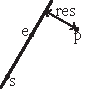
\includegraphics[width=\textwidth]{../vendor/kactl/content/geometry/lineDistance}
\end{minipage}}
\leftcaption{"Point.h"}
\begin{lstlisting}[language=C++]
template<class P>
double lineDist(P a, P b, P p) {
	return (double)(b-a).cross(p-a)/(b-a).dist();
}
\end{lstlisting}

	\KactlSnippet{SegmentDistance.h}{d5f39f, 6 lines}
\defdescription{
\begin{minipage}[t]{75mm}\vspace{0pt}
Returns the shortest distance between point p and the line segment from point s to e.
\end{minipage}
\begin{minipage}[t]{15mm}\vspace{0pt}

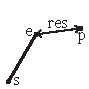
\includegraphics[width=\textwidth]{../vendor/kactl/content/geometry/SegmentDistance}
\end{minipage}}
\defusage{Point\ensuremath{<}double\ensuremath{>} a, b(2,2), p(1,1);\\
bool onSegment = segDist(a,b,p) \ensuremath{<} 1e-10;}
\leftcaption{"Point.h"}
\begin{lstlisting}[language=C++]
typedef Point<double> P;
double segDist(P s, P e, P p) {
	if (s==e) return (p-s).dist();
	auto d = (e-s).dist2(), t = min(d,max(.0,(p-s).dot(e-s)));
	return ((p-s)*d-(e-s)*t).dist()/d;
}
\end{lstlisting}

	\KactlSnippet{SegmentIntersection.h}{9d57f2, 13 lines}
\defdescription{
\begin{minipage}[t]{75mm}\vspace{0pt}
If a unique intersection point between the line segments going from s1 to e1 and from s2 to e2 exists then it is returned.
If no intersection point exists an empty vector is returned.
If infinitely many exist a vector with 2 elements is returned, containing the endpoints of the common line segment.
The wrong position will be returned if P is Point\ensuremath{<}ll\ensuremath{>} and the intersection point does not have integer coordinates.
Products of three coordinates are used in intermediate steps so watch out for overflow if using int or long long.
\end{minipage}
\begin{minipage}[t]{15mm}\vspace{0pt}
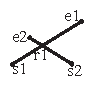
\includegraphics[width=\textwidth]{../vendor/kactl/content/geometry/SegmentIntersection}
\end{minipage}}
\defusage{vector\ensuremath{<}P\ensuremath{>} inter = segInter(s1,e1,s2,e2);\\
if (sz(inter)==1)\\
cout \ensuremath{<}\ensuremath{<} "segments intersect at " \ensuremath{<}\ensuremath{<} inter[0] \ensuremath{<}\ensuremath{<} endl;}
\leftcaption{"Point.h", "OnSegment.h"}
\begin{lstlisting}[language=C++]
template<class P> vector<P> segInter(P a, P b, P c, P d) {
	auto oa = c.cross(d, a), ob = c.cross(d, b),
	     oc = a.cross(b, c), od = a.cross(b, d);
	// Checks if intersection is single non-endpoint point.
	if (sgn(oa) * sgn(ob) < 0 && sgn(oc) * sgn(od) < 0)
		return {(a * ob - b * oa) / (ob - oa)};
	set<P> s;
	if (onSegment(c, d, a)) s.insert(a);
	if (onSegment(c, d, b)) s.insert(b);
	if (onSegment(a, b, c)) s.insert(c);
	if (onSegment(a, b, d)) s.insert(d);
	return {all(s)};
}
\end{lstlisting}

	\KactlSnippet{lineIntersection.h}{a01f81, 8 lines}
\defdescription{
\begin{minipage}[t]{75mm}\vspace{0pt}
If a unique intersection point of the lines going through s1,e1 and s2,e2 exists \{1, point\} is returned.
If no intersection point exists \{0, (0,0)\} is returned and if infinitely many exists \{-1, (0,0)\} is returned.
The wrong position will be returned if P is Point\ensuremath{<}ll\ensuremath{>} and the intersection point does not have integer coordinates.
Products of three coordinates are used in intermediate steps so watch out for overflow if using int or ll.
\end{minipage}
\begin{minipage}[t]{15mm}\vspace{0pt}
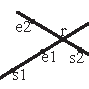
\includegraphics[width=\textwidth]{../vendor/kactl/content/geometry/lineIntersection}
\end{minipage}}
\defusage{auto res = lineInter(s1,e1,s2,e2);\\
if (res.first == 1)\\
cout \ensuremath{<}\ensuremath{<} "intersection point at " \ensuremath{<}\ensuremath{<} res.second \ensuremath{<}\ensuremath{<} endl;}
\leftcaption{"Point.h"}
\begin{lstlisting}[language=C++]
template<class P>
pair<int, P> lineInter(P s1, P e1, P s2, P e2) {
	auto d = (e1 - s1).cross(e2 - s2);
	if (d == 0) // if parallel
		return {-(s1.cross(e1, s2) == 0), P(0, 0)};
	auto p = s2.cross(e1, e2), q = s2.cross(e2, s1);
	return {1, (s1 * p + e1 * q) / d};
}
\end{lstlisting}

	\KactlSnippet{sideOf.h}{ca4665, 9 lines}
\defdescription{Returns where $p$ is as seen from $s$ towards $e$. 1/0/-1 $\Leftrightarrow$ left/on line/right.
If the optional argument $eps$ is given 0 is returned if $p$ is within distance $eps$ from the line.
P is supposed to be Point\ensuremath{<}T\ensuremath{>} where T is e.g. double or long long.
It uses products in intermediate steps so watch out for overflow if using int or long long.}
\defusage{bool left = sideOf(p1,p2,q)==1;}
\leftcaption{"Point.h"}
\begin{lstlisting}[language=C++]
template<class P>
int sideOf(P s, P e, P p) { return sgn(s.cross(e, p)); }

template<class P>
int sideOf(P s, P e, P p, double eps) {
	auto a = (e-s).cross(p-s);
	double l = (e-s).dist()*eps;
	return (a > l) - (a < -l);
}
\end{lstlisting}

	\KactlSnippet{OnSegment.h}{c597e8, 3 lines}
\defdescription{Returns true iff p lies on the line segment from s to e.
Use \texttt{(segDist(s,e,p)\ensuremath{<}=epsilon)} instead when using Point\ensuremath{<}double\ensuremath{>}.}
\leftcaption{"Point.h"}
\begin{lstlisting}[language=C++]
template<class P> bool onSegment(P s, P e, P p) {
	return p.cross(s, e) == 0 && (s - p).dot(e - p) <= 0;
}
\end{lstlisting}

	\KactlSnippet{linearTransformation.h}{7871e9, 5 lines}
\defdescription{
\begin{minipage}[t]{75mm}\vspace{0pt}
Apply the linear transformation (translation, rotation and scaling) which takes line p0-p1 to line q0-q1 to point r.
\end{minipage}
\begin{minipage}[t]{15mm}\vspace{0pt}

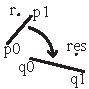
\includegraphics[width=\textwidth]{../vendor/kactl/content/geometry/linearTransformation}

\end{minipage}}
\leftcaption{"Point.h"}
\begin{lstlisting}[language=C++]
typedef Point<double> P;
P linearTransformation(P p0, P p1, P q0, P q1, P r) {
	P dp = p1-p0, dq = q1-q0, num(dp.cross(dq), dp.dot(dq));
	return q0 + P((r-p0).cross(num), (r-p0).dot(num))/dp.dist2();
}
\end{lstlisting}

	\KactlSnippet{Angle.h}{0f0602, 35 lines}
\defdescription{A class for ordering angles (as represented by int points and
a number of rotations around the origin). Useful for rotational sweeping.
Sometimes also represents points or vectors.}
\defusage{vector\ensuremath{<}Angle\ensuremath{>} v = \{w[0], w[0].t360() ...\}; // sorted\\
int j = 0; rep(i,0,n) \{ while (v[j] \ensuremath{<} v[i].t180()) ++j; \}\\
// sweeps j such that (j-i) represents the number of positively oriented triangles with vertices at 0 and i}
\begin{lstlisting}[language=C++]
struct Angle {
	int x, y;
	int t;
	Angle(int x, int y, int t=0) : x(x), y(y), t(t) {}
	Angle operator-(Angle b) const { return {x-b.x, y-b.y, t}; }
	int half() const {
		assert(x || y);
		return y < 0 || (y == 0 && x < 0);
	}
	Angle t90() const { return {-y, x, t + (half() && x >= 0)}; }
	Angle t180() const { return {-x, -y, t + half()}; }
	Angle t360() const { return {x, y, t + 1}; }
};
bool operator<(Angle a, Angle b) {
	// add a.dist2() and b.dist2() to also compare distances
	return make_tuple(a.t, a.half(), a.y * (ll)b.x) <
	       make_tuple(b.t, b.half(), a.x * (ll)b.y);
}

// Given two points, this calculates the smallest angle between
// them, i.e., the angle that covers the defined line segment.
pair<Angle, Angle> segmentAngles(Angle a, Angle b) {
	if (b < a) swap(a, b);
	return (b < a.t180() ?
	        make_pair(a, b) : make_pair(b, a.t360()));
}
Angle operator+(Angle a, Angle b) { // point a + vector b
	Angle r(a.x + b.x, a.y + b.y, a.t);
	if (a.t180() < r) r.t--;
	return r.t180() < a ? r.t360() : r;
}
Angle angleDiff(Angle a, Angle b) { // angle b - angle a
	int tu = b.t - a.t; a.t = b.t;
	return {a.x*b.x + a.y*b.y, a.x*b.y - a.y*b.x, tu - (b < a)};
}
\end{lstlisting}


\subsection{Circles}
	\KactlSnippet{CircleIntersection.h}{84d6d3, 11 lines}
\defdescription{Computes the pair of points at which two circles intersect.
Returns false in case of no intersection.}
\leftcaption{"Point.h"}
\begin{lstlisting}[language=C++]
typedef Point<double> P;
bool circleInter(P a,P b,double r1,double r2,pair<P, P>* out) {
	if (a == b) { assert(r1 != r2); return false; }
	P vec = b - a;
	double d2 = vec.dist2(), sum = r1+r2, dif = r1-r2,
	       p = (d2 + r1*r1 - r2*r2)/(d2*2), h2 = r1*r1 - p*p*d2;
	if (sum*sum < d2 || dif*dif > d2) return false;
	P mid = a + vec*p, per = vec.perp() * sqrt(fmax(0, h2) / d2);
	*out = {mid + per, mid - per};
	return true;
}
\end{lstlisting}

	\KactlSnippet{CircleTangents.h}{b0153d, 13 lines}
\defdescription{Finds the external tangents of two circles, or internal if r2 is negated.
Can return 0, 1, or 2 tangents -- 0 if one circle contains the other (or overlaps it, in the internal case, or if the circles are the same);
1 if the circles are tangent to each other (in which case .first = .second and the tangent line is perpendicular to the line between the centers).
.first and .second give the tangency points at circle 1 and 2 respectively.
To find the tangents of a circle with a point set r2 to 0.}
\leftcaption{"Point.h"}
\begin{lstlisting}[language=C++]
template<class P>
vector<pair<P, P>> tangents(P c1, double r1, P c2, double r2) {
	P d = c2 - c1;
	double dr = r1 - r2, d2 = d.dist2(), h2 = d2 - dr * dr;
	if (d2 == 0 || h2 < 0)  return {};
	vector<pair<P, P>> out;
	for (double sign : {-1, 1}) {
		P v = (d * dr + d.perp() * sqrt(h2) * sign) / d2;
		out.push_back({c1 + v * r1, c2 + v * r2});
	}
	if (h2 == 0) out.pop_back();
	return out;
}
\end{lstlisting}

	\KactlSnippet{CirclePolygonIntersection.h}{19add1, 19 lines}
\defdescription{Returns the area of the intersection of a circle with a
ccw polygon.}
\deftime{\bigo{n}}
\leftcaption{"../../content/geometry/Point.h"}
\begin{lstlisting}[language=C++]
typedef Point<double> P;
#define arg(p, q) atan2(p.cross(q), p.dot(q))
double circlePoly(P c, double r, vector<P> ps) {
	auto tri = [&](P p, P q) {
		auto r2 = r * r / 2;
		P d = q - p;
		auto a = d.dot(p)/d.dist2(), b = (p.dist2()-r*r)/d.dist2();
		auto det = a * a - b;
		if (det <= 0) return arg(p, q) * r2;
		auto s = max(0., -a-sqrt(det)), t = min(1., -a+sqrt(det));
		if (t < 0 || 1 <= s) return arg(p, q) * r2;
		P u = p + d * s, v = q + d * (t-1);
		return arg(p,u) * r2 + u.cross(v)/2 + arg(v,q) * r2;
	};
	auto sum = 0.0;
	rep(i,0,sz(ps))
		sum += tri(ps[i] - c, ps[(i + 1) % sz(ps)] - c);
	return sum;
}
\end{lstlisting}

	\KactlSnippet{circumcircle.h}{6cffc5, 9 lines}
\defdescription{
\begin{minipage}[t]{75mm}\vspace{0pt}
The circumcirle of a triangle is the circle intersecting all three vertices. ccRadius returns the radius of the circle going through points A, B and C and ccCenter returns the center of the same circle.
\end{minipage}
\begin{minipage}[t]{15mm}\vspace{0pt}

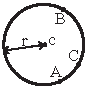
\includegraphics[width=\textwidth]{../vendor/kactl/content/geometry/circumcircle}
\end{minipage}}
\leftcaption{"Point.h"}
\begin{lstlisting}[language=C++]
typedef Point<double> P;
double ccRadius(P A, P B, P C) {
	return (B-A).dist()*(C-B).dist()*(A-C).dist()/
			abs((B-A).cross(C-A))/2;
}
P ccCenter(P A, P B, P C) {
	P b = C-A, c = B-A;
	return A + (b*c.dist2()-c*b.dist2()).perp()/b.cross(c)/2;
}
\end{lstlisting}

	\KactlSnippet{MinimumEnclosingCircle.h}{09dd0a, 17 lines}
\defdescription{Computes the minimum circle that encloses a set of points.}
\deftime{expected \bigo{n}}
\leftcaption{"circumcircle.h"}
\begin{lstlisting}[language=C++]
pair<P, double> mec(vector<P> ps) {
	shuffle(all(ps), mt19937(time(0)));
	P o = ps[0];
	double r = 0, EPS = 1 + 1e-8;
	rep(i,0,sz(ps)) if ((o - ps[i]).dist() > r * EPS) {
		o = ps[i], r = 0;
		rep(j,0,i) if ((o - ps[j]).dist() > r * EPS) {
			o = (ps[i] + ps[j]) / 2;
			r = (o - ps[i]).dist();
			rep(k,0,j) if ((o - ps[k]).dist() > r * EPS) {
				o = ccCenter(ps[i], ps[j], ps[k]);
				r = (o - ps[i]).dist();
			}
		}
	}
	return {o, r};
}
\end{lstlisting}


\subsection{Polygons}
	\KactlSnippet{InsidePolygon.h}{2bf504, 11 lines}
\defdescription{Returns true if p lies within the polygon. If strict is true,
it returns false for points on the boundary. The algorithm uses
products in intermediate steps so watch out for overflow.}
\defusage{vector\ensuremath{<}P\ensuremath{>} v = \{P\{4,4\}, P\{1,2\}, P\{2,1\}\};\\
bool in = inPolygon(v, P\{3, 3\}, false);}
\deftime{\bigo{n}}
\leftcaption{"Point.h", "OnSegment.h", "SegmentDistance.h"}
\begin{lstlisting}[language=C++]
template<class P>
bool inPolygon(vector<P> &p, P a, bool strict = true) {
	int cnt = 0, n = sz(p);
	rep(i,0,n) {
		P q = p[(i + 1) % n];
		if (onSegment(p[i], q, a)) return !strict;
		//or: if (segDist(p[i], q, a) <= eps) return !strict;
		cnt ^= ((a.y<p[i].y) - (a.y<q.y)) * a.cross(p[i], q) > 0;
	}
	return cnt;
}
\end{lstlisting}

	\KactlSnippet{PolygonArea.h}{f12300, 6 lines}
\defdescription{Returns twice the signed area of a polygon.
Clockwise enumeration gives negative area. Watch out for overflow if using int as T!}
\leftcaption{"Point.h"}
\begin{lstlisting}[language=C++]
template<class T>
T polygonArea2(vector<Point<T>>& v) {
	T a = v.back().cross(v[0]);
	rep(i,0,sz(v)-1) a += v[i].cross(v[i+1]);
	return a;
}
\end{lstlisting}

	\KactlSnippet{PolygonCenter.h}{9706dc, 9 lines}
\defdescription{Returns the center of mass for a polygon.}
\deftime{\bigo{n}}
\leftcaption{"Point.h"}
\begin{lstlisting}[language=C++]
typedef Point<double> P;
P polygonCenter(const vector<P>& v) {
	P res(0, 0); double A = 0;
	for (int i = 0, j = sz(v) - 1; i < sz(v); j = i++) {
		res = res + (v[i] + v[j]) * v[j].cross(v[i]);
		A += v[j].cross(v[i]);
	}
	return res / A / 3;
}
\end{lstlisting}

	\KactlSnippet{PolygonCut.h}{d07181, 13 lines}
\defdescription{
\begin{minipage}[t]{75mm}\vspace{0pt}
Returns a vector with the vertices of a polygon with everything to the left of the line going from s to e cut away.
\end{minipage}
\begin{minipage}[t]{15mm}\vspace{0pt}

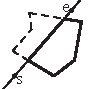
\includegraphics[width=\textwidth]{../vendor/kactl/content/geometry/PolygonCut}

\end{minipage}}
\defusage{vector\ensuremath{<}P\ensuremath{>} p = ...;\\
p = polygonCut(p, P(0,0), P(1,0));}
\leftcaption{"Point.h"}
\begin{lstlisting}[language=C++]
typedef Point<double> P;
vector<P> polygonCut(const vector<P>& poly, P s, P e) {
	vector<P> res;
	rep(i,0,sz(poly)) {
		P cur = poly[i], prev = i ? poly[i-1] : poly.back();
		auto a = s.cross(e, cur), b = s.cross(e, prev);
		if ((a < 0) != (b < 0))
			res.push_back(cur + (prev - cur) * (a / (a - b)));
		if (a < 0)
			res.push_back(cur);
	}
	return res;
}
\end{lstlisting}

	\KactlSnippet{ConvexHull.h}{310954, 13 lines}
\defdescription{\begin{minipage}[t]{75mm}\vspace{0pt}
Returns a vector of the points of the convex hull in counter-clockwise order.
Points on the edge of the hull between two other points are not considered part of the hull.
\end{minipage}
\begin{minipage}[t]{15mm}\vspace{0pt}

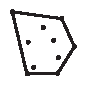
\includegraphics[width=\textwidth]{../vendor/kactl/content/geometry/ConvexHull}

\end{minipage}}
\deftime{\bigo{n \log n}}
\leftcaption{"Point.h"}
\begin{lstlisting}[language=C++]
typedef Point<ll> P;
vector<P> convexHull(vector<P> pts) {
	if (sz(pts) <= 1) return pts;
	sort(all(pts));
	vector<P> h(sz(pts)+1);
	int s = 0, t = 0;
	for (int it = 2; it--; s = --t, reverse(all(pts)))
		for (P p : pts) {
			while (t >= s + 2 && h[t-2].cross(h[t-1], p) <= 0) t--;
			h[t++] = p;
		}
	return {h.begin(), h.begin() + t - (t == 2 && h[0] == h[1])};
}
\end{lstlisting}

	\KactlSnippet{HullDiameter.h}{c571b8, 12 lines}
\defdescription{Returns the two points with max distance on a convex hull (ccw,
no duplicate/collinear points).}
\deftime{\bigo{n}}
\leftcaption{"Point.h"}
\begin{lstlisting}[language=C++]
typedef Point<ll> P;
array<P, 2> hullDiameter(vector<P> S) {
	int n = sz(S), j = n < 2 ? 0 : 1;
	pair<ll, array<P, 2>> res({0, {S[0], S[0]}});
	rep(i,0,j)
		for (;; j = (j + 1) % n) {
			res = max(res, {(S[i] - S[j]).dist2(), {S[i], S[j]}});
			if ((S[(j + 1) % n] - S[j]).cross(S[i + 1] - S[i]) >= 0)
				break;
		}
	return res.second;
}
\end{lstlisting}

	\KactlSnippet{PointInsideHull.h}{71446b, 14 lines}
\defdescription{Determine whether a point t lies inside a convex hull (CCW
order, with no collinear points). Returns true if point lies within
the hull. If strict is true, points on the boundary aren't included.}
\deftime{\bigo{\log N}}
\leftcaption{"Point.h", "sideOf.h", "OnSegment.h"}
\begin{lstlisting}[language=C++]
typedef Point<ll> P;

bool inHull(const vector<P>& l, P p, bool strict = true) {
	int a = 1, b = sz(l) - 1, r = !strict;
	if (sz(l) < 3) return r && onSegment(l[0], l.back(), p);
	if (sideOf(l[0], l[a], l[b]) > 0) swap(a, b);
	if (sideOf(l[0], l[a], p) >= r || sideOf(l[0], l[b], p)<= -r)
		return false;
	while (abs(a - b) > 1) {
		int c = (a + b) / 2;
		(sideOf(l[0], l[c], p) > 0 ? b : a) = c;
	}
	return sgn(l[a].cross(l[b], p)) < r;
}
\end{lstlisting}

	\KactlSnippet{LineHullIntersection.h}{7cf45b, 39 lines}
\defdescription{Line-convex polygon intersection. The polygon must be ccw and have no collinear points.
lineHull(line, poly) returns a pair describing the intersection of a line with the polygon:
\begin{itemize*}
\item $(-1, -1)$ if no collision,
\item $(i, -1)$ if touching the corner $i$,
\item $(i, i)$ if along side $(i, i+1)$,
\item $(i, j)$ if crossing sides $(i, i+1)$ and $(j, j+1)$.
\end{itemize*}
In the last case, if a corner $i$ is crossed, this is treated as happening on side $(i, i+1)$.
The points are returned in the same order as the line hits the polygon.
\texttt{extrVertex} returns the point of a hull with the max projection onto a line.}
\deftime{\bigo{\log n}}
\leftcaption{"Point.h"}
\begin{lstlisting}[language=C++]
#define cmp(i,j) sgn(dir.perp().cross(poly[(i)%n]-poly[(j)%n]))
#define extr(i) cmp(i + 1, i) >= 0 && cmp(i, i - 1 + n) < 0
template <class P> int extrVertex(vector<P>& poly, P dir) {
	int n = sz(poly), lo = 0, hi = n;
	if (extr(0)) return 0;
	while (lo + 1 < hi) {
		int m = (lo + hi) / 2;
		if (extr(m)) return m;
		int ls = cmp(lo + 1, lo), ms = cmp(m + 1, m);
		(ls < ms || (ls == ms && ls == cmp(lo, m)) ? hi : lo) = m;
	}
	return lo;
}

#define cmpL(i) sgn(a.cross(poly[i], b))
template <class P>
array<int, 2> lineHull(P a, P b, vector<P>& poly) {
	int endA = extrVertex(poly, (a - b).perp());
	int endB = extrVertex(poly, (b - a).perp());
	if (cmpL(endA) < 0 || cmpL(endB) > 0)
		return {-1, -1};
	array<int, 2> res;
	rep(i,0,2) {
		int lo = endB, hi = endA, n = sz(poly);
		while ((lo + 1) % n != hi) {
			int m = ((lo + hi + (lo < hi ? 0 : n)) / 2) % n;
			(cmpL(m) == cmpL(endB) ? lo : hi) = m;
		}
		res[i] = (lo + !cmpL(hi)) % n;
		swap(endA, endB);
	}
	if (res[0] == res[1]) return {res[0], -1};
	if (!cmpL(res[0]) && !cmpL(res[1]))
		switch ((res[0] - res[1] + sz(poly) + 1) % sz(poly)) {
			case 0: return {res[0], res[0]};
			case 2: return {res[1], res[1]};
		}
	return res;
}
\end{lstlisting}


\subsection{Misc. Point Set Problems}
	\KactlSnippet{ClosestPair.h}{ac41a6, 17 lines}
\defdescription{Finds the closest pair of points.}
\deftime{\bigo{n \log n}}
\leftcaption{"Point.h"}
\begin{lstlisting}[language=C++]
typedef Point<ll> P;
pair<P, P> closest(vector<P> v) {
	assert(sz(v) > 1);
	set<P> S;
	sort(all(v), [](P a, P b) { return a.y < b.y; });
	pair<ll, pair<P, P>> ret{LLONG_MAX, {P(), P()}};
	int j = 0;
	for (P p : v) {
		P d{1 + (ll)sqrt(ret.first), 0};
		while (v[j].y <= p.y - d.x) S.erase(v[j++]);
		auto lo = S.lower_bound(p - d), hi = S.upper_bound(p + d);
		for (; lo != hi; ++lo)
			ret = min(ret, {(*lo - p).dist2(), {*lo, p}});
		S.insert(p);
	}
	return ret.second;
}
\end{lstlisting}

	\KactlSnippet{kdTree.h}{69ff55, 63 lines}
\defdescription{KD-tree (2d, can be extended to 3d)}
\leftcaption{"Point.h"}
\begin{lstlisting}[language=C++]
typedef long long T;
typedef Point<T> P;
const T INF = numeric_limits<T>::max();

bool on_x(P a, P b) { return a.x < b.x; }
bool on_y(P a, P b) { return a.y < b.y; }

struct Node {
	P pt; // if this is a leaf, the single point in it
	T x0 = INF, x1 = -INF, y0 = INF, y1 = -INF; // bounds
	Node *first = 0, *second = 0;

	T distance(P p) { // min squared distance to a point
		T x = (p.x < x0 ? x0 : p.x > x1 ? x1 : p.x);
		T y = (p.y < y0 ? y0 : p.y > y1 ? y1 : p.y);
		return (P(x,y) - p).dist2();
	}

	Node(vector<P>&& vp) : pt(vp[0]) {
		for (P p : vp) {
			x0 = min(x0, p.x); x1 = max(x1, p.x);
			y0 = min(y0, p.y); y1 = max(y1, p.y);
		}
		if (vp.size() > 1) {
			// split on x if width >= height (not ideal...)
			sort(all(vp), x1 - x0 >= y1 - y0 ? on_x : on_y);
			// divide by taking half the array for each child (not
			// best performance with many duplicates in the middle)
			int half = sz(vp)/2;
			first = new Node({vp.begin(), vp.begin() + half});
			second = new Node({vp.begin() + half, vp.end()});
		}
	}
};

struct KDTree {
	Node* root;
	KDTree(const vector<P>& vp) : root(new Node({all(vp)})) {}

	pair<T, P> search(Node *node, P p) {
		if (!node->first) {
			// uncomment if we should not find the point itself:
			// if (p == node->pt) return {INF, P()};
			return make_pair((p - node->pt).dist2(), node->pt);
		}

		Node *f = node->first, *s = node->second;
		T bfirst = f->distance(p), bsec = s->distance(p);
		if (bfirst > bsec) swap(bsec, bfirst), swap(f, s);

		// search closest side first, other side if needed
		auto best = search(f, p);
		if (bsec < best.first)
			best = min(best, search(s, p));
		return best;
	}

	// find nearest point to a point, and its squared distance
	// (requires an arbitrary operator< for Point)
	pair<T, P> nearest(P p) {
		return search(root, p);
	}
};
\end{lstlisting}

	\KactlSnippet{FastDelaunay.h}{eefdf5, 88 lines}
\defdescription{Fast Delaunay triangulation.
Each circumcircle contains none of the input points.
There must be no duplicate points.
If all points are on a line, no triangles will be returned.
Should work for doubles as well, though there may be precision issues in 'circ'.
Returns triangles in order \{t[0][0], t[0][1], t[0][2], t[1][0], \dots\}, all counter-clockwise.}
\deftime{\bigo{n \log n}}
\leftcaption{"Point.h"}
\begin{lstlisting}[language=C++]
typedef Point<ll> P;
typedef struct Quad* Q;
typedef __int128_t lll; // (can be ll if coords are < 2e4)
P arb(LLONG_MAX,LLONG_MAX); // not equal to any other point

struct Quad {
	Q rot, o; P p = arb; bool mark;
	P& F() { return r()->p; }
	Q& r() { return rot->rot; }
	Q prev() { return rot->o->rot; }
	Q next() { return r()->prev(); }
} *H;

bool circ(P p, P a, P b, P c) { // is p in the circumcircle?
	lll p2 = p.dist2(), A = a.dist2()-p2,
	    B = b.dist2()-p2, C = c.dist2()-p2;
	return p.cross(a,b)*C + p.cross(b,c)*A + p.cross(c,a)*B > 0;
}
Q makeEdge(P orig, P dest) {
	Q r = H ? H : new Quad{new Quad{new Quad{new Quad{0}}}};
	H = r->o; r->r()->r() = r;
	rep(i,0,4) r = r->rot, r->p = arb, r->o = i & 1 ? r : r->r();
	r->p = orig; r->F() = dest;
	return r;
}
void splice(Q a, Q b) {
	swap(a->o->rot->o, b->o->rot->o); swap(a->o, b->o);
}
Q connect(Q a, Q b) {
	Q q = makeEdge(a->F(), b->p);
	splice(q, a->next());
	splice(q->r(), b);
	return q;
}

pair<Q,Q> rec(const vector<P>& s) {
	if (sz(s) <= 3) {
		Q a = makeEdge(s[0], s[1]), b = makeEdge(s[1], s.back());
		if (sz(s) == 2) return { a, a->r() };
		splice(a->r(), b);
		auto side = s[0].cross(s[1], s[2]);
		Q c = side ? connect(b, a) : 0;
		return {side < 0 ? c->r() : a, side < 0 ? c : b->r() };
	}

#define H(e) e->F(), e->p
#define valid(e) (e->F().cross(H(base)) > 0)
	Q A, B, ra, rb;
	int half = sz(s) / 2;
	tie(ra, A) = rec({all(s) - half});
	tie(B, rb) = rec({sz(s) - half + all(s)});
	while ((B->p.cross(H(A)) < 0 && (A = A->next())) ||
	       (A->p.cross(H(B)) > 0 && (B = B->r()->o)));
	Q base = connect(B->r(), A);
	if (A->p == ra->p) ra = base->r();
	if (B->p == rb->p) rb = base;

#define DEL(e, init, dir) Q e = init->dir; if (valid(e)) \
		while (circ(e->dir->F(), H(base), e->F())) { \
			Q t = e->dir; \
			splice(e, e->prev()); \
			splice(e->r(), e->r()->prev()); \
			e->o = H; H = e; e = t; \
		}
	for (;;) {
		DEL(LC, base->r(), o);  DEL(RC, base, prev());
		if (!valid(LC) && !valid(RC)) break;
		if (!valid(LC) || (valid(RC) && circ(H(RC), H(LC))))
			base = connect(RC, base->r());
		else
			base = connect(base->r(), LC->r());
	}
	return { ra, rb };
}

vector<P> triangulate(vector<P> pts) {
	sort(all(pts));  assert(unique(all(pts)) == pts.end());
	if (sz(pts) < 2) return {};
	Q e = rec(pts).first;
	vector<Q> q = {e};
	int qi = 0;
	while (e->o->F().cross(e->F(), e->p) < 0) e = e->o;
#define ADD { Q c = e; do { c->mark = 1; pts.push_back(c->p); \
	q.push_back(c->r()); c = c->next(); } while (c != e); }
	ADD; pts.clear();
	while (qi < sz(q)) if (!(e = q[qi++])->mark) ADD;
	return pts;
}
\end{lstlisting}


\subsection{3D}
	\KactlSnippet{PolyhedronVolume.h}{3058c3, 6 lines}
\defdescription{Magic formula for the volume of a polyhedron. Faces should point outwards.}
\begin{lstlisting}[language=C++]
template<class V, class L>
double signedPolyVolume(const V& p, const L& trilist) {
	double v = 0;
	for (auto i : trilist) v += p[i.a].cross(p[i.b]).dot(p[i.c]);
	return v / 6;
}
\end{lstlisting}

	\KactlSnippet{Point3D.h}{a94b7c, 31 lines}
\defdescription{Class to handle points in 3D space.
T can be e.g. double or long long.}
\begin{lstlisting}[language=C++]
template<class T> struct Point3D {
	typedef Point3D P;
	T x, y, z;
	explicit Point3D(T x=0, T y=0, T z=0) : x(x), y(y), z(z) {}
	bool operator<(P p) const {
		return tie(x, y, z) < tie(p.x, p.y, p.z); }
	bool operator==(P p) const {
		return tie(x, y, z) == tie(p.x, p.y, p.z); }
	P operator+(P p) const { return P(x+p.x, y+p.y, z+p.z); }
	P operator-(P p) const { return P(x-p.x, y-p.y, z-p.z); }
	P operator*(T d) const { return P(x*d, y*d, z*d); }
	P operator/(T d) const { return P(x/d, y/d, z/d); }
	T dot(P p) const { return x*p.x + y*p.y + z*p.z; }
	P cross(P p) const {
		return P(y*p.z - z*p.y, z*p.x - x*p.z, x*p.y - y*p.x);
	}
	T dist2() const { return x*x + y*y + z*z; }
	double dist() const { return sqrt((double)dist2()); }
	//Azimuthal angle (longitude) to x-axis in interval [-pi, pi]
	double phi() const { return atan2(y, x); }
	//Zenith angle (latitude) to the z-axis in interval [0, pi]
	double theta() const { return atan2(sqrt(x*x+y*y),z); }
	P unit() const { return *this/(T)dist(); } //makes dist()=1
	//returns unit vector normal to *this and p
	P normal(P p) const { return cross(p).unit(); }
	//returns point rotated 'angle' radians ccw around axis
	P rotate(double angle, P axis) const {
		double s = sin(angle), c = cos(angle); P u = axis.unit();
		return u*dot(u)*(1-c) + (*this)*c - cross(u)*s;
	}
};
\end{lstlisting}

	\KactlSnippet{3dHull.h}{5b45fc, 49 lines}
\defdescription{Computes all faces of the 3-dimension hull of a point set.
*No four points must be coplanar*, or else random results will be returned.
All faces will point outwards.}
\deftime{\bigo{n^2}}
\leftcaption{"Point3D.h"}
\begin{lstlisting}[language=C++]
typedef Point3D<double> P3;

struct PR {
	void ins(int x) { (a == -1 ? a : b) = x; }
	void rem(int x) { (a == x ? a : b) = -1; }
	int cnt() { return (a != -1) + (b != -1); }
	int a, b;
};

struct F { P3 q; int a, b, c; };

vector<F> hull3d(const vector<P3>& A) {
	assert(sz(A) >= 4);
	vector<vector<PR>> E(sz(A), vector<PR>(sz(A), {-1, -1}));
#define E(x,y) E[f.x][f.y]
	vector<F> FS;
	auto mf = [&](int i, int j, int k, int l) {
		P3 q = (A[j] - A[i]).cross((A[k] - A[i]));
		if (q.dot(A[l]) > q.dot(A[i]))
			q = q * -1;
		F f{q, i, j, k};
		E(a,b).ins(k); E(a,c).ins(j); E(b,c).ins(i);
		FS.push_back(f);
	};
	rep(i,0,4) rep(j,i+1,4) rep(k,j+1,4)
		mf(i, j, k, 6 - i - j - k);

	rep(i,4,sz(A)) {
		rep(j,0,sz(FS)) {
			F f = FS[j];
			if(f.q.dot(A[i]) > f.q.dot(A[f.a])) {
				E(a,b).rem(f.c);
				E(a,c).rem(f.b);
				E(b,c).rem(f.a);
				swap(FS[j--], FS.back());
				FS.pop_back();
			}
		}
		int nw = sz(FS);
		rep(j,0,nw) {
			F f = FS[j];
#define C(a, b, c) if (E(a,b).cnt() != 2) mf(f.a, f.b, i, f.c);
			C(a, b, c); C(a, c, b); C(b, c, a);
		}
	}
	for (F& it : FS) if ((A[it.b] - A[it.a]).cross(
		A[it.c] - A[it.a]).dot(it.q) <= 0) swap(it.c, it.b);
	return FS;
};
\end{lstlisting}

	\KactlSnippet{sphericalDistance.h}{611f07, 8 lines}
\defdescription{Returns the shortest distance on the sphere with radius radius between the points
with azimuthal angles (longitude) f1 ($\phi_1$) and f2 ($\phi_2$) from x axis and zenith angles
(latitude) t1 ($\theta_1$) and t2 ($\theta_2$) from z axis (0 = north pole). All angles measured
in radians. The algorithm starts by converting the spherical coordinates to cartesian coordinates
so if that is what you have you can use only the two last rows. dx*radius is then the difference
between the two points in the x direction and d*radius is the total distance between the points.}
\begin{lstlisting}[language=C++]
double sphericalDistance(double f1, double t1,
		double f2, double t2, double radius) {
	double dx = sin(t2)*cos(f2) - sin(t1)*cos(f1);
	double dy = sin(t2)*sin(f2) - sin(t1)*sin(f1);
	double dz = cos(t2) - cos(t1);
	double d = sqrt(dx*dx + dy*dy + dz*dz);
	return radius*2*asin(d/2);
}
\end{lstlisting}

\Topic{Strings}{strings}

\subsection{C++ std::string}
\ReferenceFact{Cost \& lifetime} Index/size: O(1); substr copies O(count); middle insert/erase/replace: O(n); find can be O(n*m) for pattern length m. Appending a character is amortized O(1). string\_view is a non-owning view: the source must outlive it and not invalidate its storage. Byte indexing is not Unicode character indexing.\par
\Snippet{String calls, parsing \& input}{C++}{substr(pos,count) truncates count at the end but throws if pos \textgreater{} size(). npos is unsigned: compare with string::npos; never test p \textgreater{}= 0. cctype functions require unsigned char conversion (or EOF).}
\lstinputlisting[language={C++}]{../topics/strings/cpp_strings.hpp}


\KactlSnippet{KMP.h}{d4375c, 16 lines}
\defdescription{pi[x] computes the length of the longest prefix of s that ends at x,
other than s[0...x] itself (abacaba -\ensuremath{>} 0010123).
Can be used to find all occurrences of a string.}
\deftime{\bigo{n}}
\begin{lstlisting}[language=C++]
vi pi(const string& s) {
	vi p(sz(s));
	rep(i,1,sz(s)) {
		int g = p[i-1];
		while (g && s[i] != s[g]) g = p[g-1];
		p[i] = g + (s[i] == s[g]);
	}
	return p;
}

vi match(const string& s, const string& pat) {
	vi p = pi(pat + '\0' + s), res;
	rep(i,sz(p)-sz(s),sz(p))
		if (p[i] == sz(pat)) res.push_back(i - 2 * sz(pat));
	return res;
}
\end{lstlisting}

\KactlSnippet{Zfunc.h}{ee09e2, 12 lines}
\defdescription{z[i] computes the length of the longest common prefix of s[i:] and s,
except z[0] = 0. (abacaba -\ensuremath{>} 0010301)}
\deftime{\bigo{n}}
\begin{lstlisting}[language=C++]
vi Z(const string& S) {
	vi z(sz(S));
	int l = -1, r = -1;
	rep(i,1,sz(S)) {
		z[i] = i >= r ? 0 : min(r - i, z[i - l]);
		while (i + z[i] < sz(S) && S[i + z[i]] == S[z[i]])
			z[i]++;
		if (i + z[i] > r)
			l = i, r = i + z[i];
	}
	return z;
}
\end{lstlisting}

\KactlSnippet{Manacher.h}{e7ad79, 13 lines}
\defdescription{For each position in a string, computes p[0][i] = half length of
longest even palindrome around pos i, p[1][i] = longest odd (half rounded down).}
\deftime{\bigo{N}}
\begin{lstlisting}[language=C++]
array<vi, 2> manacher(const string& s) {
	int n = sz(s);
	array<vi,2> p = {vi(n+1), vi(n)};
	rep(z,0,2) for (int i=0,l=0,r=0; i < n; i++) {
		int t = r-i+!z;
		if (i<r) p[z][i] = min(t, p[z][l+t]);
		int L = i-p[z][i], R = i+p[z][i]-!z;
		while (L>=1 && R+1<n && s[L-1] == s[R+1])
			p[z][i]++, L--, R++;
		if (R>r) l=L, r=R;
	}
	return p;
}
\end{lstlisting}

\KactlSnippet{MinRotation.h}{d07a42, 8 lines}
\defdescription{Finds the lexicographically smallest rotation of a string.}
\defusage{rotate(v.begin(), v.begin()+minRotation(v), v.end());}
\deftime{\bigo{N}}
\begin{lstlisting}[language=C++]
int minRotation(string s) {
	int a=0, N=sz(s); s += s;
	rep(b,0,N) rep(k,0,N) {
		if (a+k == b || s[a+k] < s[b+k]) {b += max(0, k-1); break;}
		if (s[a+k] > s[b+k]) { a = b; break; }
	}
	return a;
}
\end{lstlisting}

\KactlSnippet{SuffixArray.h}{635552, 22 lines}
\defdescription{Builds suffix array for a string.
\texttt{sa[i]} is the starting index of the suffix which
is $i$'th in the sorted suffix array.
The returned vector is of size $n+1$, and \texttt{sa[0] = n}.
The \texttt{lcp} array contains longest common prefixes for
neighbouring strings in the suffix array:
\texttt{lcp[i] = lcp(sa[i], sa[i-1])}, \texttt{lcp[0] = 0}.
The input string must not contain any nul chars.}
\deftime{\bigo{n \log n}}
\begin{lstlisting}[language=C++]
struct SuffixArray {
	vi sa, lcp;
	SuffixArray(string s, int lim=256) { // or vector<int>
		s.push_back(0); int n = sz(s), k = 0, a, b;
		vi x(all(s)), y(n), ws(max(n, lim));
		sa = lcp = y, iota(all(sa), 0);
		for (int j = 0, p = 0; p < n; j = max(1, j * 2), lim = p) {
			p = j, iota(all(y), n - j);
			rep(i,0,n) if (sa[i] >= j) y[p++] = sa[i] - j;
			fill(all(ws), 0);
			rep(i,0,n) ws[x[i]]++;
			rep(i,1,lim) ws[i] += ws[i - 1];
			for (int i = n; i--;) sa[--ws[x[y[i]]]] = y[i];
			swap(x, y), p = 1, x[sa[0]] = 0;
			rep(i,1,n) a = sa[i - 1], b = sa[i], x[b] =
				(y[a] == y[b] && y[a + j] == y[b + j]) ? p - 1 : p++;
		}
		for (int i = 0, j; i < n - 1; lcp[x[i++]] = k)
			for (k && k--, j = sa[x[i] - 1];
					s[i + k] == s[j + k]; k++);
	}
};
\end{lstlisting}

\KactlSnippet{SuffixTree.h}{aae0b8, 50 lines}
\defdescription{Ukkonen's algorithm for online suffix tree construction.
Each node contains indices [l, r) into the string, and a list of child nodes.
Suffixes are given by traversals of this tree, joining [l, r) substrings.
The root is 0 (has l = -1, r = 0), non-existent children are -1.
To get a complete tree, append a dummy symbol -- otherwise it may contain
an incomplete path (still useful for substring matching, though).}
\deftime{$\bigo{26N}$}
\begin{lstlisting}[language=C++]
struct SuffixTree {
	enum { N = 200010, ALPHA = 26 }; // N ~ 2*maxlen+10
	int toi(char c) { return c - 'a'; }
	string a; // v = cur node, q = cur position
	int t[N][ALPHA],l[N],r[N],p[N],s[N],v=0,q=0,m=2;

	void ukkadd(int i, int c) { suff:
		if (r[v]<=q) {
			if (t[v][c]==-1) { t[v][c]=m;  l[m]=i;
				p[m++]=v; v=s[v]; q=r[v];  goto suff; }
			v=t[v][c]; q=l[v];
		}
		if (q==-1 || c==toi(a[q])) q++; else {
			l[m+1]=i;  p[m+1]=m;  l[m]=l[v];  r[m]=q;
			p[m]=p[v];  t[m][c]=m+1;  t[m][toi(a[q])]=v;
			l[v]=q;  p[v]=m;  t[p[m]][toi(a[l[m]])]=m;
			v=s[p[m]];  q=l[m];
			while (q<r[m]) { v=t[v][toi(a[q])];  q+=r[v]-l[v]; }
			if (q==r[m])  s[m]=v;  else s[m]=m+2;
			q=r[v]-(q-r[m]);  m+=2;  goto suff;
		}
	}

	SuffixTree(string a) : a(a) {
		fill(r,r+N,sz(a));
		memset(s, 0, sizeof s);
		memset(t, -1, sizeof t);
		fill(t[1],t[1]+ALPHA,0);
		s[0] = 1; l[0] = l[1] = -1; r[0] = r[1] = p[0] = p[1] = 0;
		rep(i,0,sz(a)) ukkadd(i, toi(a[i]));
	}

	// example: find longest common substring (uses ALPHA = 28)
	pii best;
	int lcs(int node, int i1, int i2, int olen) {
		if (l[node] <= i1 && i1 < r[node]) return 1;
		if (l[node] <= i2 && i2 < r[node]) return 2;
		int mask = 0, len = node ? olen + (r[node] - l[node]) : 0;
		rep(c,0,ALPHA) if (t[node][c] != -1)
			mask |= lcs(t[node][c], i1, i2, len);
		if (mask == 3)
			best = max(best, {len, r[node] - len});
		return mask;
	}
	static pii LCS(string s, string t) {
		SuffixTree st(s + (char)('z' + 1) + t + (char)('z' + 2));
		st.lcs(0, sz(s), sz(s) + 1 + sz(t), 0);
		return st.best;
	}
};
\end{lstlisting}

\KactlSnippet{Hashing.h}{2d2a67, 44 lines}
\defdescription{Self-explanatory methods for string hashing.}
\begin{lstlisting}[language=C++]
// Arithmetic mod 2^64-1. 2x slower than mod 2^64 and more
// code, but works on evil test data (e.g. Thue-Morse, where
// ABBA... and BAAB... of length 2^10 hash the same mod 2^64).
// "typedef ull H;" instead if you think test data is random,
// or work mod 10^9+7 if the Birthday paradox is not a problem.
typedef uint64_t ull;
struct H {
	ull x; H(ull x=0) : x(x) {}
	H operator+(H o) { return x + o.x + (x + o.x < x); }
	H operator-(H o) { return *this + ~o.x; }
	H operator*(H o) { auto m = (__uint128_t)x * o.x;
		return H((ull)m) + (ull)(m >> 64); }
	ull get() const { return x + !~x; }
	bool operator==(H o) const { return get() == o.get(); }
	bool operator<(H o) const { return get() < o.get(); }
};
static const H C = (ll)1e11+3; // (order ~ 3e9; random also ok)

struct HashInterval {
	vector<H> ha, pw;
	HashInterval(string& str) : ha(sz(str)+1), pw(ha) {
		pw[0] = 1;
		rep(i,0,sz(str))
			ha[i+1] = ha[i] * C + str[i],
			pw[i+1] = pw[i] * C;
	}
	H hashInterval(int a, int b) { // hash [a, b)
		return ha[b] - ha[a] * pw[b - a];
	}
};

vector<H> getHashes(string& str, int length) {
	if (sz(str) < length) return {};
	H h = 0, pw = 1;
	rep(i,0,length)
		h = h * C + str[i], pw = pw * C;
	vector<H> ret = {h};
	rep(i,length,sz(str)) {
		ret.push_back(h = h * C + str[i] - pw * str[i-length]);
	}
	return ret;
}

H hashString(string& s){H h{}; for(char c:s) h=h*C+c;return h;}
\end{lstlisting}

\KactlSnippet{AhoCorasick.h}{f35677, 66 lines}
\defdescription{Aho-Corasick automaton, used for multiple pattern matching.
Initialize with AhoCorasick ac(patterns); the automaton start node will be at index 0.
find(word) returns for each position the index of the longest word that ends there, or -1 if none.
findAll($-$, word) finds all words (up to $N \sqrt N$ many if no duplicate patterns)
that start at each position (shortest first).
Duplicate patterns are allowed; empty patterns are not.
To find the longest words that start at each position, reverse all input.
For large alphabets, split each symbol into chunks, with sentinel bits for symbol boundaries.}
\deftime{construction takes $\bigo{26N}$, where $N =$ sum of length of patterns.
find(x) is $\bigo{N}$, where N = length of x. findAll is $\bigo{NM}$.}
\begin{lstlisting}[language=C++]
struct AhoCorasick {
	enum {alpha = 26, first = 'A'}; // change this!
	struct Node {
		// (nmatches is optional)
		int back, next[alpha], start = -1, end = -1, nmatches = 0;
		Node(int v) { memset(next, v, sizeof(next)); }
	};
	vector<Node> N;
	vi backp;
	void insert(string& s, int j) {
		assert(!s.empty());
		int n = 0;
		for (char c : s) {
			int& m = N[n].next[c - first];
			if (m == -1) { n = m = sz(N); N.emplace_back(-1); }
			else n = m;
		}
		if (N[n].end == -1) N[n].start = j;
		backp.push_back(N[n].end);
		N[n].end = j;
		N[n].nmatches++;
	}
	AhoCorasick(vector<string>& pat) : N(1, -1) {
		rep(i,0,sz(pat)) insert(pat[i], i);
		N[0].back = sz(N);
		N.emplace_back(0);

		queue<int> q;
		for (q.push(0); !q.empty(); q.pop()) {
			int n = q.front(), prev = N[n].back;
			rep(i,0,alpha) {
				int &ed = N[n].next[i], y = N[prev].next[i];
				if (ed == -1) ed = y;
				else {
					N[ed].back = y;
					(N[ed].end == -1 ? N[ed].end : backp[N[ed].start])
						= N[y].end;
					N[ed].nmatches += N[y].nmatches;
					q.push(ed);
				}
			}
		}
	}
	vi find(string word) {
		int n = 0;
		vi res; // ll count = 0;
		for (char c : word) {
			n = N[n].next[c - first];
			res.push_back(N[n].end);
			// count += N[n].nmatches;
		}
		return res;
	}
	vector<vi> findAll(vector<string>& pat, string word) {
		vi r = find(word);
		vector<vi> res(sz(word));
		rep(i,0,sz(word)) {
			int ind = r[i];
			while (ind != -1) {
				res[i - sz(pat[ind]) + 1].push_back(ind);
				ind = backp[ind];
			}
		}
		return res;
	}
};
\end{lstlisting}

\Topic{Search, DP \& optimization}{search-dp}

\subsection{C++ lambdas \& sorting}
\ReferenceFact{Comparator contract} comp(a,b) means a precedes b; it must be a strict weak ordering. Use \textless{}, never \textless{}=; comp(x,x) must be false. For tie breakers use tie(a.first,a.second) \textless{} tie(b.first,b.second), not subtraction (overflow). sort is unstable; stable\_sort preserves equivalent elements.\par
\ReferenceFact{Captures} [] none; [x] snapshot by value; [\&x] by reference; [=] implicit copies; [\&] implicit references; [x,\&y] mixed. mutable allows changing captured copies. Reference captures must outlive the lambda; a copied pointer still refers to the original object. Use -\textgreater{} ReturnType for explicit/recursive return types.\par
\ReferenceFact{Useful algorithms} sort and nth\_element need random-access iterators. unique removes adjacent duplicates logically and returns a new end: erase the tail. next\_permutation returns false and resets to ascending at the final permutation. min\_element/max\_element return end() for empty ranges; accumulate(...,0LL) uses a 64-bit sum.\par
\Snippet{Sorting, bounds \& lambda syntax}{C++}{All iterator ranges are half-open. stable\_sort is O(n log n) with enough extra memory, otherwise up to O(n log\textasciicircum{}2 n) comparisons. Lambda recursion shown below requires passing itself explicitly: fib(fib,n).}
\lstinputlisting[language={C++}]{../topics/search/cpp_sort_lambdas.hpp}
\subsection{Search \& dynamic programming}
\Snippet{Binary search / first true}{Python}{binary\_search requires an ascending sorted sequence; it returns any matching index or -1. first\_true requires a false-then-true predicate on integer indices in [lo, hi). Example lower bound: first\_true(0, len(a), lambda i: a[i] \textgreater{}= x). O(log n) predicate calls, O(1) auxiliary space.}
\lstinputlisting[language={Python}]{../topics/search/binary_search.py}
\Snippet{Kadane: maximum subarray sum}{Python}{O(n) time, O(1) auxiliary space. Handles all-negative input; a must be nonempty. ending is the best sum ending at the current position.}
\lstinputlisting[language={Python}]{../topics/dynamic_programming/kadane.py}
\subsection{Bit operations}
\Snippet{Parity, masks, XOR and shifts}{Java}{XOR identities: x\textasciicircum{}x=0, x\textasciicircum{}0=x. unique assumes all other values occur an even number of times. XOR swap uses distinct storage; a temporary variable is clearer. x\textless{}\textless{}k multiplies by 2\textasciicircum{}k only without overflow; signed x\textgreater{}\textgreater{}k rounds toward negative infinity, unlike Java integer division for negative values. \textgreater{}\textgreater{}\textgreater{} shifts in zero bits. int shifts mask k with 31; long shifts mask with 63. Use 1L\textless{}\textless{}bit for long masks. Bit operations are not automatically faster than equivalent arithmetic.}
\lstinputlisting[language={Java}]{../topics/bitwise/Bitwise.java}


\subsection{Intervals}
	\KactlSnippet{IntervalContainer.h}{edce47, 23 lines}
\defdescription{Add and remove intervals from a set of disjoint intervals.
Will merge the added interval with any overlapping intervals in the set when adding.
Intervals are [inclusive, exclusive).}
\deftime{\bigo{\log N}}
\begin{lstlisting}[language=C++]
set<pii>::iterator addInterval(set<pii>& is, int L, int R) {
	if (L == R) return is.end();
	auto it = is.lower_bound({L, R}), before = it;
	while (it != is.end() && it->first <= R) {
		R = max(R, it->second);
		before = it = is.erase(it);
	}
	if (it != is.begin() && (--it)->second >= L) {
		L = min(L, it->first);
		R = max(R, it->second);
		is.erase(it);
	}
	return is.insert(before, {L,R});
}

void removeInterval(set<pii>& is, int L, int R) {
	if (L == R) return;
	auto it = addInterval(is, L, R);
	auto r2 = it->second;
	if (it->first == L) is.erase(it);
	else (int&)it->second = L;
	if (R != r2) is.emplace(R, r2);
}
\end{lstlisting}

	\KactlSnippet{IntervalCover.h}{9e9d8d, 19 lines}
\defdescription{Compute indices of smallest set of intervals covering another interval.
Intervals should be [inclusive, exclusive). To support [inclusive, inclusive],
change (A) to add \texttt{|| R.empty()}. Returns empty set on failure (or if G is empty).}
\deftime{\bigo{N \log N}}
\begin{lstlisting}[language=C++]
template<class T>
vi cover(pair<T, T> G, vector<pair<T, T>> I) {
	vi S(sz(I)), R;
	iota(all(S), 0);
	sort(all(S), [&](int a, int b) { return I[a] < I[b]; });
	T cur = G.first;
	int at = 0;
	while (cur < G.second) { // (A)
		pair<T, int> mx = make_pair(cur, -1);
		while (at < sz(I) && I[S[at]].first <= cur) {
			mx = max(mx, make_pair(I[S[at]].second, S[at]));
			at++;
		}
		if (mx.second == -1) return {};
		cur = mx.first;
		R.push_back(mx.second);
	}
	return R;
}
\end{lstlisting}

	\KactlSnippet{ConstantIntervals.h}{753a4c, 19 lines}
\defdescription{Split a monotone function on [from, to) into a minimal set of half-open intervals on which it has the same value.
Runs a callback g for each such interval.}
\defusage{constantIntervals(0, sz(v), [\&](int x)\{return v[x];\}, [\&](int lo, int hi, T val)\{...\});}
\deftime{\bigo{k\log\frac{n}{k}}}
\begin{lstlisting}[language=C++]
template<class F, class G, class T>
void rec(int from, int to, F& f, G& g, int& i, T& p, T q) {
	if (p == q) return;
	if (from == to) {
		g(i, to, p);
		i = to; p = q;
	} else {
		int mid = (from + to) >> 1;
		rec(from, mid, f, g, i, p, f(mid));
		rec(mid+1, to, f, g, i, p, q);
	}
}
template<class F, class G>
void constantIntervals(int from, int to, F f, G g) {
	if (to <= from) return;
	int i = from; auto p = f(i), q = f(to-1);
	rec(from, to-1, f, g, i, p, q);
	g(i, to, q);
}
\end{lstlisting}


\subsection{Misc. algorithms}
	\KactlSnippet{TernarySearch.h}{9155b4, 11 lines}
\defdescription{Find the smallest i in $[a,b]$ that maximizes $f(i)$, assuming that $f(a) \ensuremath{<} \dots \ensuremath{<} f(i) \ge \dots \ge f(b)$.
To reverse which of the sides allows non-strict inequalities, change the \ensuremath{<} marked with (A) to \ensuremath{<}=, and reverse the loop at (B).
To minimize $f$, change it to \ensuremath{>}, also at (B).}
\defusage{int ind = ternSearch(0,n-1,[\&](int i)\{return a[i];\});}
\deftime{\bigo{\log(b-a)}}
\begin{lstlisting}[language=C++]
template<class F>
int ternSearch(int a, int b, F f) {
	assert(a <= b);
	while (b - a >= 5) {
		int mid = (a + b) / 2;
		if (f(mid) < f(mid+1)) a = mid; // (A)
		else b = mid+1;
	}
	rep(i,a+1,b+1) if (f(a) < f(i)) a = i; // (B)
	return a;
}
\end{lstlisting}

	\KactlSnippet{LIS.h}{2932a0, 17 lines}
\defdescription{Compute indices for the longest increasing subsequence.}
\deftime{$\bigo{N \log N}$}
\begin{lstlisting}[language=C++]
template<class I> vi lis(const vector<I>& S) {
	if (S.empty()) return {};
	vi prev(sz(S));
	typedef pair<I, int> p;
	vector<p> res;
	rep(i,0,sz(S)) {
		// change 0 -> i for longest non-decreasing subsequence
		auto it = lower_bound(all(res), p{S[i], 0});
		if (it == res.end()) res.emplace_back(), it = res.end()-1;
		*it = {S[i], i};
		prev[i] = it == res.begin() ? 0 : (it-1)->second;
	}
	int L = sz(res), cur = res.back().second;
	vi ans(L);
	while (L--) ans[L] = cur, cur = prev[cur];
	return ans;
}
\end{lstlisting}

	\KactlSnippet{FastKnapsack.h}{b20ccc, 16 lines}
\defdescription{Given N non-negative integer weights w and a non-negative target t,
computes the maximum S \ensuremath{<}= t such that S is the sum of some subset of the weights.}
\deftime{\bigo{N \max(w_i)}}
\begin{lstlisting}[language=C++]
int knapsack(vi w, int t) {
	int a = 0, b = 0, x;
	while (b < sz(w) && a + w[b] <= t) a += w[b++];
	if (b == sz(w)) return a;
	int m = *max_element(all(w));
	vi u, v(2*m, -1);
	v[a+m-t] = b;
	rep(i,b,sz(w)) {
		u = v;
		rep(x,0,m) v[x+w[i]] = max(v[x+w[i]], u[x]);
		for (x = 2*m; --x > m;) rep(j, max(0,u[x]), v[x])
			v[x-w[j]] = max(v[x-w[j]], j);
	}
	for (a = t; v[a+m-t] < 0; a--) ;
	return a;
}
\end{lstlisting}


\subsection{Dynamic programming}
	\KactlSnippet{KnuthDP.h}{}
\defdescription{When doing DP on intervals: $a[i][j] = \min_{i \ensuremath{<} k \ensuremath{<} j}(a[i][k] + a[k][j]) + f(i, j)$, where the (minimal) optimal $k$ increases with both $i$ and $j$,
one can solve intervals in increasing order of length, and search $k = p[i][j]$ for $a[i][j]$ only between $p[i][j-1]$ and $p[i+1][j]$.
This is known as Knuth DP. Sufficient criteria for this are if $f(b,c) \le f(a,d)$ and $f(a,c) + f(b,d) \le f(a,d) + f(b,c)$ for all $a \le b \le c \le d$.
Consider also: LineContainer (ch. Data structures), monotone queues, ternary search.}
\deftime{\bigo{N^2}}
\begin{lstlisting}[language=C++]

\end{lstlisting}

	\KactlSnippet{DivideAndConquerDP.h}{d38d2b, 18 lines}
\defdescription{Given $a[i] = \min_{lo(i) \le k \ensuremath{<} hi(i)}(f(i, k))$ where the (minimal)
optimal $k$ increases with $i$, computes $a[i]$ for $i = L..R-1$.}
\deftime{\bigo{(N + (hi-lo)) \log N}}
\begin{lstlisting}[language=C++]
struct DP { // Modify at will:
	int lo(int ind) { return 0; }
	int hi(int ind) { return ind; }
	ll f(int ind, int k) { return dp[ind][k]; }
	void store(int ind, int k, ll v) { res[ind] = pii(k, v); }

	void rec(int L, int R, int LO, int HI) {
		if (L >= R) return;
		int mid = (L + R) >> 1;
		pair<ll, int> best(LLONG_MAX, LO);
		rep(k, max(LO,lo(mid)), min(HI,hi(mid)))
			best = min(best, make_pair(f(mid, k), k));
		store(mid, best.second, best.first);
		rec(L, mid, LO, best.second+1);
		rec(mid+1, R, best.second, HI);
	}
	void solve(int L, int R) { rec(L, R, INT_MIN, INT_MAX); }
};
\end{lstlisting}


\subsection{Debugging tricks}
	\begin{itemize}
		\item \verb@signal(SIGSEGV, [](int) { _Exit(0); });@ converts segfaults into Wrong Answers.
			Similarly one can catch SIGABRT (assertion failures) and SIGFPE (zero divisions).
			\verb@_GLIBCXX_DEBUG@ failures generate SIGABRT (or SIGSEGV on gcc 5.4.0 apparently).
		\item \verb@feenableexcept(29);@ kills the program on NaNs (\texttt 1), 0-divs (\texttt 4), infinities (\texttt 8) and denormals (\texttt{16}).
	\end{itemize}

\subsection{Optimization tricks}
	\verb@__builtin_ia32_ldmxcsr(40896);@ disables denormals (which make floats 20x slower near their minimum value).
	\subsubsection{Bit hacks}
		\begin{itemize}
			\item \verb@x & -x@ is the least bit in \texttt{x}.
			\item \verb@for (int x = m; x; ) { --x &= m; ... }@ loops over all subset masks of \texttt{m} (except \texttt{m} itself).
			\item \verb@c = x&-x, r = x+c; (((r^x) >> 2)/c) | r@ is the next number after \texttt{x} with the same number of bits set.
			\item \verb@rep(b,0,K) rep(i,0,(1 << K))@ \\ \verb@  if (i & 1 << b) D[i] += D[i^(1 << b)];@ computes all sums of subsets.
		\end{itemize}
	\subsubsection{Pragmas}
		\begin{itemize}
			\item \lstinline{#pragma GCC optimize ("Ofast")} will make GCC auto-vectorize loops and optimizes floating points better.
			\item \lstinline{#pragma GCC target ("avx2")} can double performance of vectorized code, but causes crashes on old machines.
			\item \lstinline{#pragma GCC optimize ("trapv")} kills the program on integer overflows (but is really slow).
		\end{itemize}
	\KactlSnippet{FastMod.h}{751a02, 8 lines}
\defdescription{Compute $a \% b$ about 5 times faster than usual, where $b$ is constant but not known at compile time.
Returns a value congruent to $a \pmod b$ in the range $[0, 2b)$.}
\begin{lstlisting}[language=C++]
typedef unsigned long long ull;
struct FastMod {
	ull b, m;
	FastMod(ull b) : b(b), m(-1ULL / b) {}
	ull reduce(ull a) { // a % b + (0 or b)
		return a - (ull)((__uint128_t(m) * a) >> 64) * b;
	}
};
\end{lstlisting}

	\KactlSnippet{FastInput.h}{7b3c70, 17 lines}
\defdescription{Read an integer from stdin. Usage requires your program to pipe in
input from file.}
\defusage{./a.out \ensuremath{<} input.txt}
\deftime{About 5x as fast as cin/scanf.}
\begin{lstlisting}[language=C++]
inline char gc() { // like getchar()
	static char buf[1 << 16];
	static size_t bc, be;
	if (bc >= be) {
		buf[0] = 0, bc = 0;
		be = fread(buf, 1, sizeof(buf), stdin);
	}
	return buf[bc++]; // returns 0 on EOF
}

int readInt() {
	int a, c;
	while ((a = gc()) < 40);
	if (a == '-') return -readInt();
	while ((c = gc()) >= 48) a = a * 10 + c - 480;
	return a - 48;
}
\end{lstlisting}

	\KactlSnippet{BumpAllocator.h}{745db2, 8 lines}
\defdescription{When you need to dynamically allocate many objects and don't care about freeing them.
"new X" otherwise has an overhead of something like 0.05us + 16 bytes per allocation.}
\begin{lstlisting}[language=C++]
// Either globally or in a single class:
static char buf[450 << 20];
void* operator new(size_t s) {
	static size_t i = sizeof buf;
	assert(s < i);
	return (void*)&buf[i -= s];
}
void operator delete(void*) {}
\end{lstlisting}

	\KactlSnippet{SmallPtr.h}{2dd6c9, 10 lines}
\defdescription{A 32-bit pointer that points into BumpAllocator memory.}
\leftcaption{"BumpAllocator.h"}
\begin{lstlisting}[language=C++]
template<class T> struct ptr {
	unsigned ind;
	ptr(T* p = 0) : ind(p ? unsigned((char*)p - buf) : 0) {
		assert(ind < sizeof buf);
	}
	T& operator*() const { return *(T*)(buf + ind); }
	T* operator->() const { return &**this; }
	T& operator[](int a) const { return (&**this)[a]; }
	explicit operator bool() const { return ind; }
};
\end{lstlisting}

	\KactlSnippet{BumpAllocatorSTL.h}{bb66d4, 14 lines}
\defdescription{BumpAllocator for STL containers.}
\defusage{vector\ensuremath{<}vector\ensuremath{<}int, small\ensuremath{<}int\ensuremath{>}\ensuremath{>}\ensuremath{>} ed(N);}
\begin{lstlisting}[language=C++]
char buf[450 << 20] alignas(16);
size_t buf_ind = sizeof buf;

template<class T> struct small {
	typedef T value_type;
	small() {}
	template<class U> small(const U&) {}
	T* allocate(size_t n) {
		buf_ind -= n * sizeof(T);
		buf_ind &= 0 - alignof(T);
		return (T*)(buf + buf_ind);
	}
	void deallocate(T*, size_t) {}
};
\end{lstlisting}

	\KactlSnippet{SIMD.h}{c9ac08, 43 lines}
\defdescription{Cheat sheet of SSE/AVX intrinsics, for doing arithmetic on several numbers at once.
Can provide a constant factor improvement of about 4, orthogonal to loop unrolling.
Operations follow the pattern \texttt{"\_mm(256)?\_name\_(si(128|256)|epi(8|16|32|64)|pd|ps)"}. Not all are described here;
grep for \texttt{\_mm\_} in \texttt{/usr/lib/gcc/{*}/4.9/include/} for more.
If AVX is unsupported, try 128-bit operations, "emmintrin.h" and \#define \texttt{\_\_SSE\_\_} and \texttt{\_\_MMX\_\_} before including it.
For aligned memory use \texttt{\_mm\_malloc(size, 32)} or \texttt{int buf[N] alignas(32)}, but prefer loadu/storeu.}
\begin{lstlisting}[language=C++]
#pragma GCC target ("avx2") // or sse4.1
#include "immintrin.h"

typedef __m256i mi;
#define L(x) _mm256_loadu_si256((mi*)&(x))

// High-level/specific methods:
// load(u)?_si256, store(u)?_si256, setzero_si256, _mm_malloc
// blendv_(epi8|ps|pd) (z?y:x), movemask_epi8 (hibits of bytes)
// i32gather_epi32(addr, x, 4): map addr[] over 32-b parts of x
// sad_epu8: sum of absolute differences of u8, outputs 4xi64
// maddubs_epi16: dot product of unsigned i7's, outputs 16xi15
// madd_epi16: dot product of signed i16's, outputs 8xi32
// extractf128_si256(, i) (256->128), cvtsi128_si32 (128->lo32)
// permute2f128_si256(x,x,1) swaps 128-bit lanes
// shuffle_epi32(x, 3*64+2*16+1*4+0) == x for each lane
// shuffle_epi8(x, y) takes a vector instead of an imm

// Methods that work with most data types (append e.g. _epi32):
// set1, blend (i8?x:y), add, adds (sat.), mullo, sub, and/or,
// andnot, abs, min, max, sign(1,x), cmp(gt|eq), unpack(lo|hi)

int sumi32(mi m) { union {int v[8]; mi m;} u; u.m = m;
	int ret = 0; rep(i,0,8) ret += u.v[i]; return ret; }
mi zero() { return _mm256_setzero_si256(); }
mi one() { return _mm256_set1_epi32(-1); }
bool all_zero(mi m) { return _mm256_testz_si256(m, m); }
bool all_one(mi m) { return _mm256_testc_si256(m, one()); }

ll example_filteredDotProduct(int n, short* a, short* b) {
	int i = 0; ll r = 0;
	mi zero = _mm256_setzero_si256(), acc = zero;
	while (i + 16 <= n) {
		mi va = L(a[i]), vb = L(b[i]); i += 16;
		va = _mm256_and_si256(_mm256_cmpgt_epi16(vb, va), va);
		mi vp = _mm256_madd_epi16(va, vb);
		acc = _mm256_add_epi64(_mm256_unpacklo_epi32(vp, zero),
			_mm256_add_epi64(acc, _mm256_unpackhi_epi32(vp, zero)));
	}
	union {ll v[4]; mi m;} u; u.m = acc; rep(i,0,4) r += u.v[i];
	for (;i<n;++i) if (a[i] < b[i]) r += a[i]*b[i]; // <- equiv
	return r;
}
\end{lstlisting}

\Topic{Algorithm checklist}{techniques}




\KactlSnippet{techniques.txt}{159 lines}
\ReferenceFact{Recursion} \par
\ReferenceFact{Divide and conquer} Finding interesting points in N log N\par
\ReferenceFact{Algorithm analysis} Master theorem; Amortized time complexity\par
\ReferenceFact{Greedy algorithm} Scheduling; Max contiguous subvector sum; Invariants; Huffman encoding\par
\ReferenceFact{Graph theory} Dynamic graphs (extra book-keeping); Breadth first search; Depth first search; * Normal trees / DFS trees; Dijkstra's algorithm; MST: Prim's algorithm; Bellman-Ford; Konig's theorem and vertex cover; Min-cost max flow; Lovasz toggle; Matrix tree theorem; Maximal matching, general graphs; Hopcroft-Karp; Hall's marriage theorem; Graphical sequences; Floyd-Warshall; Euler cycles; Flow networks; * Augmenting paths; * Edmonds-Karp; Bipartite matching; Min. path cover; Topological sorting; Strongly connected components; 2-SAT; Cut vertices, cut-edges and biconnected components; Edge coloring; * Trees; Vertex coloring; * Bipartite graphs (=\textgreater{} trees); * 3\textasciicircum{}n (special case of set cover); Diameter and centroid; K'th shortest path; Shortest cycle\par
\ReferenceFact{Dynamic programming} Knapsack; Coin change; Longest common subsequence; Longest increasing subsequence; Number of paths in a dag; Shortest path in a dag; Dynprog over intervals; Dynprog over subsets; Dynprog over probabilities; Dynprog over trees; 3\textasciicircum{}n set cover; Divide and conquer; Knuth optimization; Convex hull optimizations; RMQ (sparse table a.k.a 2\textasciicircum{}k-jumps); Bitonic cycle; Log partitioning (loop over most restricted)\par
\ReferenceFact{Combinatorics} Computation of binomial coefficients; Pigeon-hole principle; Inclusion/exclusion; Catalan number; Pick's theorem\par
\ReferenceFact{Number theory} Integer parts; Divisibility; Euclidean algorithm; Modular arithmetic; * Modular multiplication; * Modular inverses; * Modular exponentiation by squaring; Chinese remainder theorem; Fermat's little theorem; Euler's theorem; Phi function; Frobenius number; Quadratic reciprocity; Pollard-Rho; Miller-Rabin; Hensel lifting; Vieta root jumping\par
\ReferenceFact{Game theory} Combinatorial games; Game trees; Mini-max; Nim; Games on graphs; Games on graphs with loops; Grundy numbers; Bipartite games without repetition; General games without repetition; Alpha-beta pruning\par
\ReferenceFact{Probability theory} \par
\ReferenceFact{Optimization} Binary search; Ternary search; Unimodality and convex functions; Binary search on derivative\par
\ReferenceFact{Numerical methods} Numeric integration; Newton's method; Root-finding with binary/ternary search; Golden section search\par
\ReferenceFact{Matrices} Gaussian elimination; Exponentiation by squaring\par
\ReferenceFact{Sorting} Radix sort\par
\ReferenceFact{Geometry} Coordinates and vectors; * Cross product; * Scalar product; Convex hull; Polygon cut; Closest pair; Coordinate-compression; Quadtrees; KD-trees; All segment-segment intersection\par
\ReferenceFact{Sweeping} Discretization (convert to events and sweep); Angle sweeping; Line sweeping; Discrete second derivatives\par
\ReferenceFact{Strings} Longest common substring; Palindrome subsequences; Knuth-Morris-Pratt; Tries; Rolling polynomial hashes; Suffix array; Suffix tree; Aho-Corasick; Manacher's algorithm; Letter position lists\par
\ReferenceFact{Combinatorial search} Meet in the middle; Brute-force with pruning; Best-first (A*); Bidirectional search; Iterative deepening DFS / A*\par
\ReferenceFact{Data structures} LCA (2\textasciicircum{}k-jumps in trees in general); Pull/push-technique on trees; Heavy-light decomposition; Centroid decomposition; Lazy propagation; Self-balancing trees; Convex hull trick (wcipeg.com/wiki/Convex\_hull\_trick); Monotone queues / monotone stacks / sliding queues; Sliding queue using 2 stacks; Persistent segment tree\par
\end{multicols}\label{last-page}
\end{document}
